
%DIF LATEXDIFF DIFFERENCE FILE
%DIF DEL original-submission.tex       Sun Sep 27 15:28:07 2026
%DIF ADD elsarticle-template-num.tex   Sun Sep 27 07:35:09 2026
\documentclass[preprint,12pt]{elsarticle}




%% The amsmath package provides various useful equation environments.
\usepackage{amsmath}    % align, cases, etc.
\usepackage{amssymb}    % math symbols
\usepackage{mathtools}  % fixes + extensions to amsmath

%% The amsthm package provides extended theorem environments
\usepackage{amsthm}
\usepackage{hyperref}
\usepackage{adjustbox}
\usepackage{siunitx} %  for better scientific notation
\usepackage{booktabs}
\usepackage{longtable }
\usepackage{graphicx}
\usepackage{subcaption} % for subfigures
\usepackage{algorithm}
\usepackage{algorithmic}

\newtheorem{definition}{Definition}[section]
\newtheorem{theorem}{Theorem}[section]
\newtheorem{lemma}{Lemma}[section]
%DIF 27a27
\newtheorem{corollary}[lemma]{Corollary} %DIF > 
%DIF -------
\newtheorem{assumption}{Assumption}[section]
\usepackage{lineno}

\journal{Reliability Engineering \& System Safety}
%DIF PREAMBLE EXTENSION ADDED BY LATEXDIFF
%DIF UNDERLINE PREAMBLE %DIF PREAMBLE
\RequirePackage[normalem]{ulem} %DIF PREAMBLE
\RequirePackage{color}\definecolor{RED}{rgb}{1,0,0}\definecolor{BLUE}{rgb}{0,0,1} %DIF PREAMBLE
\providecommand{\DIFaddtex}[1]{{\protect\color{blue}\uwave{#1}}} %DIF PREAMBLE
\providecommand{\DIFdeltex}[1]{{\protect\color{red}\sout{#1}}} %DIF PREAMBLE
%DIF SAFE PREAMBLE %DIF PREAMBLE
\providecommand{\DIFaddbegin}{} %DIF PREAMBLE
\providecommand{\DIFaddend}{} %DIF PREAMBLE
\providecommand{\DIFdelbegin}{} %DIF PREAMBLE
\providecommand{\DIFdelend}{} %DIF PREAMBLE
\providecommand{\DIFmodbegin}{} %DIF PREAMBLE
\providecommand{\DIFmodend}{} %DIF PREAMBLE
%DIF FLOATSAFE PREAMBLE %DIF PREAMBLE
\providecommand{\DIFaddFL}[1]{\DIFadd{#1}} %DIF PREAMBLE
\providecommand{\DIFdelFL}[1]{\DIFdel{#1}} %DIF PREAMBLE
\providecommand{\DIFaddbeginFL}{} %DIF PREAMBLE
\providecommand{\DIFaddendFL}{} %DIF PREAMBLE
\providecommand{\DIFdelbeginFL}{} %DIF PREAMBLE
\providecommand{\DIFdelendFL}{} %DIF PREAMBLE
%DIF HYPERREF PREAMBLE %DIF PREAMBLE
\providecommand{\DIFadd}[1]{\texorpdfstring{\DIFaddtex{#1}}{#1}} %DIF PREAMBLE
\providecommand{\DIFdel}[1]{\texorpdfstring{\DIFdeltex{#1}}{}} %DIF PREAMBLE
\providecommand{\DIFscaledelfig}{0.5}
%DIF HIGHLIGHTGRAPHICS PREAMBLE %DIF PREAMBLE
\RequirePackage{settobox} %DIF PREAMBLE
\RequirePackage{letltxmacro} %DIF PREAMBLE
\newsavebox{\DIFdelgraphicsbox} %DIF PREAMBLE
\newlength{\DIFdelgraphicswidth} %DIF PREAMBLE
\newlength{\DIFdelgraphicsheight} %DIF PREAMBLE
% store original definition of \includegraphics %DIF PREAMBLE
\LetLtxMacro{\DIFOincludegraphics}{\includegraphics} %DIF PREAMBLE
\providecommand{\DIFaddincludegraphics}[2][]{{\color{blue}\fbox{\DIFOincludegraphics[#1]{#2}}}} %DIF PREAMBLE
\providecommand{\DIFdelincludegraphics}[2][]{% %DIF PREAMBLE
\sbox{\DIFdelgraphicsbox}{\DIFOincludegraphics[#1]{#2}}% %DIF PREAMBLE
\settoboxwidth{\DIFdelgraphicswidth}{\DIFdelgraphicsbox} %DIF PREAMBLE
\settoboxtotalheight{\DIFdelgraphicsheight}{\DIFdelgraphicsbox} %DIF PREAMBLE
\scalebox{\DIFscaledelfig}{% %DIF PREAMBLE
\parbox[b]{\DIFdelgraphicswidth}{\usebox{\DIFdelgraphicsbox}\\[-\baselineskip] \rule{\DIFdelgraphicswidth}{0em}}\llap{\resizebox{\DIFdelgraphicswidth}{\DIFdelgraphicsheight}{% %DIF PREAMBLE
\setlength{\unitlength}{\DIFdelgraphicswidth}% %DIF PREAMBLE
\begin{picture}(1,1)% %DIF PREAMBLE
\thicklines\linethickness{2pt} %DIF PREAMBLE
{\color[rgb]{1,0,0}\put(0,0){\framebox(1,1){}}}% %DIF PREAMBLE
{\color[rgb]{1,0,0}\put(0,0){\line( 1,1){1}}}% %DIF PREAMBLE
{\color[rgb]{1,0,0}\put(0,1){\line(1,-1){1}}}% %DIF PREAMBLE
\end{picture}% %DIF PREAMBLE
}\hspace*{3pt}}} %DIF PREAMBLE
} %DIF PREAMBLE
\LetLtxMacro{\DIFOaddbegin}{\DIFaddbegin} %DIF PREAMBLE
\LetLtxMacro{\DIFOaddend}{\DIFaddend} %DIF PREAMBLE
\LetLtxMacro{\DIFOdelbegin}{\DIFdelbegin} %DIF PREAMBLE
\LetLtxMacro{\DIFOdelend}{\DIFdelend} %DIF PREAMBLE
\DeclareRobustCommand{\DIFaddbegin}{\DIFOaddbegin \let\includegraphics\DIFaddincludegraphics} %DIF PREAMBLE
\DeclareRobustCommand{\DIFaddend}{\DIFOaddend \let\includegraphics\DIFOincludegraphics} %DIF PREAMBLE
\DeclareRobustCommand{\DIFdelbegin}{\DIFOdelbegin \let\includegraphics\DIFdelincludegraphics} %DIF PREAMBLE
\DeclareRobustCommand{\DIFdelend}{\DIFOaddend \let\includegraphics\DIFOincludegraphics} %DIF PREAMBLE
\LetLtxMacro{\DIFOaddbeginFL}{\DIFaddbeginFL} %DIF PREAMBLE
\LetLtxMacro{\DIFOaddendFL}{\DIFaddendFL} %DIF PREAMBLE
\LetLtxMacro{\DIFOdelbeginFL}{\DIFdelbeginFL} %DIF PREAMBLE
\LetLtxMacro{\DIFOdelendFL}{\DIFdelendFL} %DIF PREAMBLE
\DeclareRobustCommand{\DIFaddbeginFL}{\DIFOaddbeginFL \let\includegraphics\DIFaddincludegraphics} %DIF PREAMBLE
\DeclareRobustCommand{\DIFaddendFL}{\DIFOaddendFL \let\includegraphics\DIFOincludegraphics} %DIF PREAMBLE
\DeclareRobustCommand{\DIFdelbeginFL}{\DIFOdelbeginFL \let\includegraphics\DIFdelincludegraphics} %DIF PREAMBLE
\DeclareRobustCommand{\DIFdelendFL}{\DIFOaddendFL \let\includegraphics\DIFOincludegraphics} %DIF PREAMBLE
%DIF AMSMATHULEM PREAMBLE %DIF PREAMBLE
\makeatletter %DIF PREAMBLE
\let\sout@orig\sout %DIF PREAMBLE
\renewcommand{\sout}[1]{\ifmmode\text{\sout@orig{\ensuremath{#1}}}\else\sout@orig{#1}\fi} %DIF PREAMBLE
\makeatother %DIF PREAMBLE
%DIF COLORLISTINGS PREAMBLE %DIF PREAMBLE
\RequirePackage{listings} %DIF PREAMBLE
\RequirePackage{color} %DIF PREAMBLE
\lstdefinelanguage{DIFcode}{ %DIF PREAMBLE
%DIF DIFCODE_UNDERLINE %DIF PREAMBLE
  moredelim=[il][\color{red}\sout]{\%DIF\ <\ }, %DIF PREAMBLE
  moredelim=[il][\color{blue}\uwave]{\%DIF\ >\ } %DIF PREAMBLE
} %DIF PREAMBLE
\lstdefinestyle{DIFverbatimstyle}{ %DIF PREAMBLE
	language=DIFcode, %DIF PREAMBLE
	basicstyle=\ttfamily, %DIF PREAMBLE
	columns=fullflexible, %DIF PREAMBLE
	keepspaces=true %DIF PREAMBLE
} %DIF PREAMBLE
\lstnewenvironment{DIFverbatim}[1][]{\lstset{style=DIFverbatimstyle}}{} %DIF PREAMBLE
\lstnewenvironment{DIFverbatim*}[1][]{\lstset{style=DIFverbatimstyle,showspaces=true}}{} %DIF PREAMBLE
\lstset{extendedchars=\true,inputencoding=utf8}

%DIF END PREAMBLE EXTENSION ADDED BY LATEXDIFF

\begin{document}
\linenumbers

\begin{frontmatter}


\title{Information Propagation Algorithm for Exact Reliability Analysis in Directed Acyclic Process Networks}

\author[strathclyde]{Temitope Ohiani}\ead{temitope.ohiani@strath.ac.uk}
\author[strathclyde]{Edoardo Patelli\corref{mycorrespondingauthor}} \ead{edoardo.patelli@strath.ac.uk}
\author[nnl]{Caroline Pyke}\ead{caroline.pyke@uknnl.com}

\affiliation[strathclyde]{organization={Department of Civil and Environmental Engineering, University of Strathclyde},
            city={Glasgow},
            country={UK}}

\affiliation[nnl]{organization={United Kingdom National Nuclear Laboratory},
            country={UK}}

  \cortext[mycorrespondingauthor]{Corresponding author}


%% Abstract
\begin{abstract}
Reliability analysis in directed acyclic process networks requires computing, for each node, the probability that at least one viable path exists from any source node to that node. Standard analytical reliability formulations become inaccurate or inefficient in the presence of reconvergent path structures, where multiple paths diverge from shared upstream ancestors and reconverge downstream, thereby creating statistical dependencies that violate path independence assumptions.

This paper presents the Information Propagation Algorithm (IPA), an exact message-passing method that resolves these dependencies through conditional enumeration on shared fork ancestors. IPA processes the network in topological order, applying closed-form updates for independent parent signals and progressive diamond decomposition for dependent reconvergent structures. \DIFdelbegin \DIFdel{Diamond subgraphs are systematically identified, solved through }\DIFdelend \DIFaddbegin \DIFadd{IPA identifies each diamond subgraph, solves it by }\DIFaddend conditional probability enumeration, and \DIFdelbegin \DIFdel{replaced with statistically equivalent supernodes, thereby avoiding repeated conditioningover previously resolved structures}\DIFdelend \DIFaddbegin \DIFadd{replaces it with a statistically equivalent supernode. IPA is a specialisation of cutset conditioning, and its cost is computed from the decomposition before the propagation is run}\DIFaddend .

\DIFdelbegin \DIFdel{Two case studies are used to evaluate the proposed method. On a 16-node }\DIFdelend \DIFaddbegin \DIFadd{IPA also propagates interval-valued and probability-box component reliabilities. For interval inputs the propagated range is exact, and for probability-box inputs the bounds on each node's reliability distribution are guaranteed. IPA is validated against an independent binary decision diagram on a benchmark }\DIFaddend grid network, \DIFdelbegin \DIFdel{IPA reproduces exact reliability values and achieves a 134-fold reduction in runtime relative to a published message-passing alternative. Analysis of six Pareto-optimal }\DIFdelend \DIFaddbegin \DIFadd{power, gas, transit, and water distribution networks, and a corpus of 129 random and structured directed acyclic graphs. It reproduces the exact node reliabilities in every case. It is then applied to a medical }\DIFaddend drone logistics network \DIFdelbegin \DIFdel{configurations shows that computation time depends primarily on diamond nesting depth rather than network size: shallow-nested networks (depth $\leq 12$) are solved in under one second, whereas deeply nested structures exhibit the exponential growth inherent to exact inference in high-treewidth graphs. The results demonstrate that IPA provides an exact and computationally efficient reliability analysis tool }\DIFdelend \DIFaddbegin \DIFadd{for Scotland. The analysis identifies the delivery points whose reachability is least certain under the stated input uncertainty. IPA provides exact reliability analysis }\DIFaddend for a broad class of multi-source directed acyclic process \DIFdelbegin \DIFdel{systems, while also identifying }\DIFdelend \DIFaddbegin \DIFadd{networks, and identifies }\DIFaddend the structural conditions under which exact inference becomes impractical.
\end{abstract}

%%Research highlights
\begin{highlights}
\item Exact \DIFdelbegin \DIFdel{reliability computation for directed acyclic process networks with reconvergent dependencies
}\DIFdelend \DIFaddbegin \DIFadd{source-to-node reliability for DAGs with reconvergent (diamond) dependence
}\DIFaddend \item \DIFdelbegin \DIFdel{Resolves dependent fork--join structures through conditional decomposition on shared upstream nodes
}\DIFdelend \DIFaddbegin \DIFadd{Diamond decomposition with supernode reuse avoids repeated conditioning
}\DIFaddend \item \DIFdelbegin \DIFdel{Uses progressive diamond decomposition and supernode replacement to avoid repeated dependency evaluation
}\DIFdelend \DIFaddbegin \DIFadd{Per-instance cost follows from the diamond conditioning sets and is known in advance
}\DIFaddend \item \DIFdelbegin \DIFdel{Reproduces exact benchmark results and is substantially faster than a published message-passing alternative
}\DIFdelend \DIFaddbegin \DIFadd{Validated against an exact decision-diagram method on 129 graphs and benchmarks
}\DIFaddend \item \DIFdelbegin \DIFdel{Demonstrates that practical tractability is governed primarily by diamond nesting depth rather than network size
}\DIFdelend \DIFaddbegin \DIFadd{Propagates interval and probability-box component reliabilities natively
}\DIFaddend \end{highlights}


%% Keywords
\begin{keyword}
Network Reliability \sep Directed Acyclic Graphs \sep Message Passing \sep Reconvergent Structures \sep \DIFaddbegin \DIFadd{Imprecise Probability }\sep \DIFaddend Process Networks \sep Infrastructure Systems
\end{keyword}

\end{frontmatter}

%% Add \usepackage{lineno} before \begin{document} and uncomment 
%% following line to enable line numbers
%% \linenumbers

%% main text
%%


\section{Introduction}

Many infrastructure and engineered systems operate through the propagation of resources \DIFdelbegin \DIFdel{, services, or }\DIFdelend \DIFaddbegin \DIFadd{and }\DIFaddend information across interconnected components. Examples include electric power networks, water distribution systems, telecommunication networks, transportation systems, and logistics networks. In such systems, functionality depends \DIFdelbegin \DIFdel{not only }\DIFdelend on the reliability of individual components \DIFdelbegin \DIFdel{but also }\DIFdelend \DIFaddbegin \DIFadd{and }\DIFaddend on the existence of viable directed paths through which flow can propagate from source nodes to downstream nodes. In this paper, we refer to this class of systems as \emph{multi-source process networks}.
Failures in these systems can have severe operational, economic, environmental, and societal consequences. Their assessment therefore requires metrics that quantify \DIFdelbegin \DIFdel{not only component reliability but also the ability of the network}\DIFdelend \DIFaddbegin \DIFadd{component reliability and the network's ability }\DIFaddend to preserve connectivity and sustain flow. A natural reliability measure in this context is the probability that at least one viable path exists from one or more source nodes to a given target node. This source-to-node reachability reliability provides a direct measure of the network's ability to maintain function under component and transmission failures.

Directed acyclic graphs (DAGs) are a natural fit to model and evaluate the performance of resource flow systems. In a DAG, nodes represent system components, processing stages, or transfer locations, while directed edges model permissible flow transition\DIFaddbegin \DIFadd{s}\DIFaddend  and dependencies between components. Consider the typical process of transport networks where service at downstream locations may depend on the successful operation of several upstream links, hubs, or transfer stages. Failures at earlier stations can cause disruption and delays in travel and, in some cases, stop service altogether.

\DIFdelbegin \DIFdel{To mitigate }\DIFdelend \DIFaddbegin \DIFadd{Monitoring this reliability is what allows }\DIFaddend cascading failure scenarios and service bottlenecks \DIFdelbegin \DIFdel{, the reliability of the network's resource flow is an important performance metric to monitor. Reliability is generally defined as the probability that a system performs its intended function over a specified time. In flow networks, the intended function is that the other parts of the network successfully receive information flowing from the sources. Complex systems have }\DIFdelend \DIFaddbegin \DIFadd{to be anticipated and mitigated. Complex systems typically rely on }\DIFaddend redundancy strategies and backup paths to \DIFdelbegin \DIFdel{ensure this flow . Reliability in multi-source flow networks is related to the probability that at least one viable operational path exists from source nodes to the other nodes in the network.
}\DIFdelend \DIFaddbegin \DIFadd{sustain flow when individual components fail.
}\DIFaddend 

The classic approach to exactly solving the reliability problem involves enumerating and combining all possible source-to-node paths. However, this quickly becomes computationally intractable for complex process systems with multiple sources, extensive redundancy, and re-convergent network topologies \cite{george-williams_simulation_2021}. In particular, when distinct paths share upstream nodes or edges before reconverging downstream, the resulting path events are no longer independent, and naïve path-combination rules become invalid.

The structure of DAGs suggests an alternative viewpoint based on message passing. \DIFdelbegin \DIFdel{Rather than globally enumerating all viable paths, reliability }\DIFdelend \DIFaddbegin \DIFadd{Reliability }\DIFaddend can be computed locally and recursively by asking, at each node\DIFdelbegin \DIFdel{: }\emph{\DIFdel{what is the probability that at least one viable signal reaches this node from any source?}}%DIFAUXCMD
\DIFdelend \DIFaddbegin \DIFadd{, the probability that at least one viable signal reaches it from any source}\DIFaddend . For tree-like or conditionally independent substructures, this can be evaluated efficiently using local update rules. However, reconvergent path structures remain problematic because they induce statistical dependencies between incoming signals. These dependencies must be resolved exactly if message passing is to remain accurate.

This paper presents the \emph{Information Propagation Algorithm} (IPA), an exact message-passing method for reliability analysis in directed acyclic process networks. IPA exploits topological ordering to propagate source-to-node reliability from upstream to downstream nodes. Its central idea is to identify reconvergent fork--join subgraphs, referred to here as \emph{diamond structures}, and resolve their dependency explicitly by conditioning on the shared fork ancestors. Once solved, these diamond subgraphs are replaced with statistically equivalent supernodes, \DIFdelbegin \DIFdel{allowing the network to be }\DIFdelend \DIFaddbegin \DIFadd{and the network is }\DIFaddend progressively simplified without loss of exactness. \DIFaddbegin \DIFadd{An earlier version of the method was presented as the Information Propagation Method~\mbox{%DIFAUXCMD
\cite{ohiani_information_2023}}\hskip0pt%DIFAUXCMD
. This paper adds a formal complexity analysis, a validation against an independent exact method, and the propagation of imprecise component reliabilities.
}\DIFaddend 

The proposed approach \DIFdelbegin \DIFdel{present several advantages: it preserves exact reliability computation }\DIFdelend \DIFaddbegin \DIFadd{preserves exact probability propagation }\DIFaddend in DAGs with reconvergent structures, \DIFdelbegin \DIFdel{avoiding the independence errors that arise from }\DIFdelend \DIFaddbegin \DIFadd{where the }\DIFaddend standard local update \DIFdelbegin \DIFdel{rules; by decomposing }\DIFdelend \DIFaddbegin \DIFadd{introduces an independence error. Decomposing }\DIFaddend and caching repeated dependency patterns \DIFdelbegin \DIFdel{, it reduces repeated }\DIFdelend \DIFaddbegin \DIFadd{reduces }\DIFaddend conditional enumeration over already-resolved substructures\DIFdelbegin \DIFdel{; and being based on analytical methods, the algorithm allows to analyse large systems in nearly real-time making it adaptable during design phases where multiple analysisof the system under different configurations need to be tested as well for supporting decision tools of critical systems that required a fast assessment of the systems}\DIFdelend \DIFaddbegin \DIFadd{. The cost on a given network is fixed by the decomposition and known before enumeration begins. The approach also propagates interval-valued and probability-box component reliabilities, so that partial knowledge of the component data is carried through the analysis. These properties suit the method to design-stage studies, where many network configurations are assessed, and to decision problems where the reliability inputs are only partly known}\DIFaddend .


\subsection{Related Works}\label{subsec:relatedworks}

Early reliability analysis methods are based on relatively simple structural representations of systems. \DIFaddbegin \DIFadd{The }\DIFaddend Reliability Block Diagram (RBD) \DIFdelbegin \DIFdel{\mbox{%DIFAUXCMD
\cite{billinton_network_1992,rausand_m_2014_reliability_2014,ebeling_introduction_2019} }\hskip0pt%DIFAUXCMD
methodmodels }\DIFdelend \DIFaddbegin \DIFadd{method~\mbox{%DIFAUXCMD
\cite{billinton_network_1992,rausand_m_2014_reliability_2014,ebeling_introduction_2019} }\hskip0pt%DIFAUXCMD
models a }\DIFaddend system as interconnected component blocks arranged in series, parallel, or $k$-out-of-$n$ configurations, whose reliability can be computed using closed-form expressions. While computationally efficient and intuitive, RBDs are limited in their ability to represent complex dependency structures and reconvergent flows. Extensions such as Dynamic Reliability Block Diagrams (DRBD)\DIFaddbegin \DIFadd{~}\DIFaddend \cite{distefano_dynamic_2007} incorporate time-dependent behaviour and \DIFdelbegin \DIFdel{allowing for }\DIFdelend \DIFaddbegin \DIFadd{allow }\DIFaddend more realistic modelling of component interactions and system dependencies\DIFaddbegin \DIFadd{, }\DIFaddend but they still struggle to represent highly interconnected networks with multiple convergent paths.

Boolean logic-based methods provide a more flexible framework for modelling system failure mechanisms by including event causes and consequences. Fault Tree Analysis (FTA) \cite{xing_fault_2008} is a top-down deductive logic tree to identify possible combinations of component failures that could cause specific undesirable events. Event Tree Analysis (ETA) is the complementary inductive method where the logic tree instead begins with the initiating event and \DIFdelbegin \DIFdel{systematically }\DIFdelend traces all possible sequences of subsequent successes and failures through branching structures and logic gates \cite{cepin_event_2011}. These methods can capture a wider range of logical dependencies than RBDs; however, for large-scale systems they require extensive manual construction and become difficult to maintain. In addition, their computational cost grows rapidly with the size and complexity of the logical expressions, particularly in systems with multiple interacting pathways~\cite{sherwin_fault_1993,xing_fault_2008}.

The main limitations of tree-based methods stem from exponential growth in logic expressions and manual construction requirements for complex systems. Binary Decision Diagrams (BDDs)\cite{rauzy_new_1993,bryant_graph-based_1986, brace_efficient_1990} were adapted from circuit design to improve fault tree models by using variable elimination and path reduction techniques on Boolean functions. In BDDs, Boolean functions are represented as directed acyclic graphs (DAGs) based on Shannon decomposition, where each non-sink node represents a Boolean variable with two outgoing edges corresponding to the variable being true or false \cite{xing_fault_2008}. This structure allows BDD-based methods to require less memory and computational time than traditional fault tree analysis \cite{rauzy_new_1993}.
BDD algorithms can handle complex Boolean expressions with thousands of variables\DIFdelbegin \DIFdel{while maintaining polynomial space complexity }\DIFdelend \DIFaddbegin \DIFadd{, keeping the diagram's size polynomial }\DIFaddend for many systems \DIFdelbegin \DIFdel{. However, their performance depends critically on variable ordering, and determining }\DIFdelend \DIFaddbegin \DIFadd{under a favourable variable ordering. Determining }\DIFaddend an optimal ordering is itself computationally intractable in general~\cite{bryant_ordered_nodate}\DIFaddbegin \DIFadd{, and a poor ordering can make the diagram grow exponentially instead}\DIFaddend . For highly interconnected networks with shared components and reconvergent \DIFdelbegin \DIFdel{fanout structures, optimal variable ordering becomes computationally intractable. 
BDD construction for networks with diamond structures - where multiple independent paths converge }\DIFdelend \DIFaddbegin \DIFadd{fan-out, BDD construction meets the reconvergence problem. Multiple paths converging }\DIFaddend at common nodes \DIFdelbegin \DIFdel{- suffers from the reconvergence problem, requiring }\DIFdelend \DIFaddbegin \DIFadd{require }\DIFaddend extensive intermediate node generation\DIFdelbegin \DIFdel{that }\DIFdelend \DIFaddbegin \DIFadd{, which }\DIFaddend can exceed memory limitations even for moderately sized systems. These \DIFdelbegin \DIFdel{computational challenges become particularly }\DIFdelend \DIFaddbegin \DIFadd{challenges become }\DIFaddend severe when modelling common cause failures and \DIFdelbegin \DIFdel{complex }\DIFdelend dependency structures that propagate through \DIFdelbegin \DIFdel{multiple interconnected pathwayssimultaneously}\DIFdelend \DIFaddbegin \DIFadd{many interconnected pathways}\DIFaddend .

Common cause failures create statistical dependencies that violate the independence assumptions underlying traditional reliability calculations\cite{mosleh_estimation_nodate}. When multiple components share common failure modes, the resulting dependency patterns cannot be \DIFdelbegin \DIFdel{efficiently captured }\DIFdelend \DIFaddbegin \DIFadd{captured efficiently }\DIFaddend through simple Boolean combinations\DIFdelbegin \DIFdel{, representing a fundamental }\DIFdelend \DIFaddbegin \DIFadd{. This is a }\DIFaddend limitation shared by RBDs, FTAs, and BDDs in process systems with convergent network topologies.

To overcome these limitations, path-based and graph-theoretic methods have been developed. These methods \DIFdelbegin \DIFdel{contextualise }\DIFdelend \DIFaddbegin \DIFadd{treat }\DIFaddend the network as a probabilistic graph \DIFdelbegin \DIFdel{theory problem and leverage }\DIFdelend \DIFaddbegin \DIFadd{problem and apply }\DIFaddend probability mathematics and set operations to \DIFdelbegin \DIFdel{calculate }\DIFdelend \DIFaddbegin \DIFadd{compute }\DIFaddend network reliability. Exact methods based on minimal path sets and minimal cut sets~\DIFdelbegin \DIFdel{\mbox{%DIFAUXCMD
\cite{kumar_composite_2018,li_cuttie_2005,billinton_network_1992, liu_improved_2012} }\hskip0pt%DIFAUXCMD
}\DIFdelend \DIFaddbegin \DIFadd{\mbox{%DIFAUXCMD
\cite{kumar_composite_2018,li_cuttie_2005,billinton_network_1992,liu_improved_2012} }\hskip0pt%DIFAUXCMD
}\DIFaddend identify the smallest collections of components that \DIFdelbegin \DIFdel{ensure connectivity or guarantee }\DIFdelend \DIFaddbegin \DIFadd{maintain connectivity or cause }\DIFaddend system failure. Recursive decomposition techniques \DIFdelbegin \DIFdel{further }\DIFdelend improve efficiency by partitioning the network into smaller subproblems. For example, the cut-based method in\DIFdelbegin \DIFdel{\mbox{%DIFAUXCMD
\cite{liu_improved_2012} }\hskip0pt%DIFAUXCMD
proposes simultaneously using }\DIFdelend \DIFaddbegin \DIFadd{~\mbox{%DIFAUXCMD
\cite{liu_improved_2012} }\hskip0pt%DIFAUXCMD
uses }\DIFaddend both the disjoint minimal cut sets and \DIFaddbegin \DIFadd{the }\DIFaddend disjoint minimal path sets during \DIFdelbegin \DIFdel{the decomposition process }\DIFdelend \DIFaddbegin \DIFadd{decomposition }\DIFaddend for networks with low edge reliabilities. Kim and Kang's method \cite{kim_network_2013} extends the Recursive Decomposition Algorithm through a Logical Expansion approach (LE-RDA) that uses \DIFdelbegin \DIFdel{two separate procedures for }\DIFdelend \DIFaddbegin \DIFadd{separate }\DIFaddend intersection and union \DIFdelbegin \DIFdel{logical functions to handle decomposition of }\DIFdelend \DIFaddbegin \DIFadd{operations to decompose }\DIFaddend general system events with multiple node pairs. Nevertheless, these methods remain computationally expensive for networks with extensive redundancy and reconvergent connectivity, as they still require combinatorial enumeration of path or cut structures.

Simulation methods such as Monte Carlo (MC) have become \DIFdelbegin \DIFdel{a widely adopted reliability analysis method for }\DIFdelend \DIFaddbegin \DIFadd{widely adopted for reliability analysis of }\DIFaddend complex networks \cite{fishman_comparison_1986}. MC algorithms can handle arbitrary network structures and provide confidence intervals, although they can become computationally expensive for large networks requiring many samples to reach acceptable accuracy. Monte Carlo variants such as importance sampling\cite{hui_monte_2007} and subset simulation \cite{au_estimation_2001} have been proposed to address rare failure events, though these optimisations often demand more computational cost\DIFdelbegin \DIFdel{s}\DIFdelend  .

More recently, message passing approaches based on probabilistic graphical models have been explored for network reliability analysis~\cite{yedidia_understanding_2003,pearl_probabilistic_1988}. These methods infer \DIFdelbegin \DIFdel{the reliability of the system }\DIFdelend \DIFaddbegin \DIFadd{system reliability }\DIFaddend by exploiting the network structure to propagate \DIFdelbegin \DIFdel{the local calculations throughout the network }\DIFdelend \DIFaddbegin \DIFadd{local calculations }\DIFaddend until convergence. \DIFdelbegin \DIFdel{Unlike enumeration-based methods, message }\DIFdelend \DIFaddbegin \DIFadd{Message }\DIFaddend passing scales linearly with network size and \DIFdelbegin \DIFdel{naturally }\DIFdelend handles complex dependency structures \DIFaddbegin \DIFadd{directly}\DIFaddend . For instance, \DIFdelbegin \DIFdel{method for system reliability such as }\DIFdelend the directed Probability Propagation Method (dPrPm)~\cite{tong_probability_2019} \DIFdelbegin \DIFdel{, also allows to handle }\DIFdelend \DIFaddbegin \DIFadd{handles }\DIFaddend dependencies through pairwise probability tracking and approximation of joint distributions. While effective, these approaches can become memory-intensive and computationally demanding as the number of dependent interactions increases. In addition, convergence is not always guaranteed~\cite{murphy_loopy_2013}, and approximation quality depends heavily on network topology and component correlation strength.

\DIFaddbegin \DIFadd{Exact inference in probabilistic graphical models resolves a dependency induced by shared ancestry either by conditioning or by clustering. Cutset conditioning enumerates the states of a set of variables whose removal leaves the rest of the structure singly connected~\mbox{%DIFAUXCMD
\cite{pearl_probabilistic_1988}}\hskip0pt%DIFAUXCMD
. The junction-tree algorithm groups variables into a tree of clusters, and its cost is exponential in the treewidth of the network~\mbox{%DIFAUXCMD
\cite{lauritzen_local_1988}}\hskip0pt%DIFAUXCMD
. Both are exact, and both are governed by a structural width of the graph. IPA specialises cutset conditioning to the source-to-node reachability problem, and its cost is governed by the same width parameter as junction-tree inference and a well-ordered binary decision diagram (Section~\ref{sec:complexity}).
}

\DIFadd{A component failure probability is often known only within bounds, from sparse operational data or expert judgement. Such a value is represented as an interval, asserting only that the true reliability lies between two bounds, or as a probability box, a pair of bounding cumulative distribution functions~\mbox{%DIFAUXCMD
\cite{ferson_constructing_2003}}\hskip0pt%DIFAUXCMD
. Williamson and Downs~\mbox{%DIFAUXCMD
\cite{williamson_probabilistic_1990} }\hskip0pt%DIFAUXCMD
give the arithmetic on probability boxes under known or unknown dependence, on the classical Fr\'echet--Hoeffding bounds for joint distributions. A binary decision diagram can be extended to interval-valued inputs, using the same monotonicity IPA relies on~\mbox{%DIFAUXCMD
\cite{jacob_uncertainty_2011}}\hskip0pt%DIFAUXCMD
. The construction does not scale. Its result also depends on the variable ordering, so a conservative envelope over several orderings is needed~\mbox{%DIFAUXCMD
\cite{imakhlaf_extending_2017}}\hskip0pt%DIFAUXCMD
. IPA propagates interval and probability-box reliabilities through the same conditioning it applies to point values, without an ordering or a separate monotonicity check.
}

\DIFaddend Hence, existing methods face a trade-off between generality, computational efficiency, and exactness. Classical analytical methods struggle with complex dependency structures, exact path-based approaches suffer from combinatorial explosion, and simulation or approximate message-passing methods sacrifice exactness for scalability. This work addresses this gap by proposing an exact message-passing framework for DAG reliability analysis that explicitly resolves reconvergent dependencies through conditional decomposition of fork--join substructures. By identifying and reducing these structures during computation, the proposed method avoids repeated enumeration over shared dependencies \DIFdelbegin \DIFdel{while preserving }\DIFdelend \DIFaddbegin \DIFadd{and preserves }\DIFaddend exact probabilistic results.

\section{Network Model}\DIFaddbegin \label{sec:model}
\DIFaddend A process system \DIFdelbegin \DIFdel{is }\DIFdelend \DIFaddbegin \DIFadd{can be }\DIFaddend modelled as a directed acyclic graph $G = (V, E)$ where $V$ denotes the set of nodes (components) and $E \subseteq V \times V$ represents the set of directed edges (dependencies). Let $S \subseteq V$ denote the \DIFdelbegin \DIFdel{sets of source and  $T \subseteq V$ the sink }\DIFdelend \DIFaddbegin \DIFadd{set of source }\DIFaddend nodes. Throughout the paper we use $\text{Pa}(v)$ \DIFdelbegin \DIFdel{and $\text{Ch}(v)$ }\DIFdelend to represent the set of parent nodes \DIFdelbegin \DIFdel{and child nodes }\DIFdelend of $v$\DIFdelbegin \DIFdel{, respectively}\DIFdelend .

\subsection{Component States and Probabilistic Model}

Each node $v \in V$ is associated with a binary random variable $X_v \in \{0,1\}$, where $X_v = 1$ indicates that node $v$ is operational. Similarly, each directed edge $(u,v) \in E$ is associated with a binary random variable $X_{uv} \in \{0,1\}$ representing successful transmission from $u$ to $v$.

We define:
\begin{itemize}
\item $R(v) = P(X_v = 1)$: intrinsic reliability of node $v$
\item $P(u,v) = P(X_{uv} = 1)$: transmission probability of edge $(u,v)$
\end{itemize}

A directed path $\pi(s,v) = (s = v_0, v_1, \ldots, v_k = v)$ is said to be \emph{viable} if all nodes and edges along the path are operational, i.e.
\[
X_{v_0} X_{v_1} \cdots X_{v_k} \cdot X_{v_0 v_1} \cdots X_{v_{k-1} v_k} = 1.
\]

\begin{definition}[Viable Path]
A path $\pi(s,v)$ from source $s \in S$ to node $v \in V$ is viable if all nodes and edges along the path are functional.
\end{definition}

\begin{figure}[htbp]
  \centering
  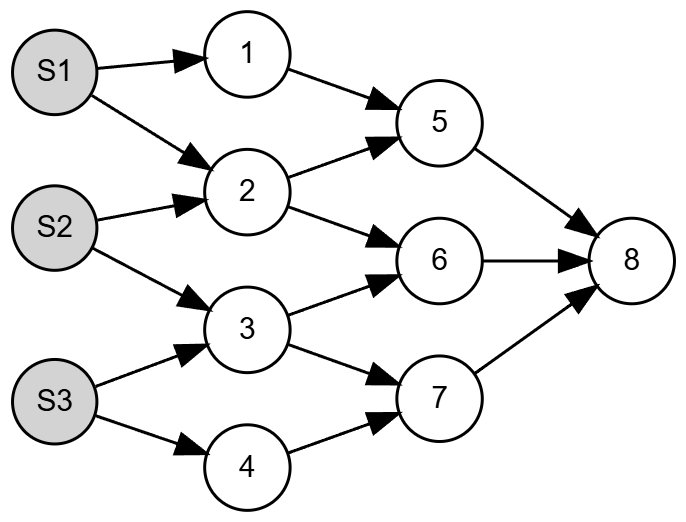
\includegraphics[scale=0.3]{images/simpleDag.png}
  \caption{A Multi-Source Directed Acyclic Graph.}
  \label{fig:dag_rbd}
\end{figure}

\subsection{Definition of Diamond Structures}

We formalise reconvergent dependency patterns through the \DIFdelbegin \DIFdel{notion }\DIFdelend \DIFaddbegin \DIFadd{concept }\DIFaddend of a diamond subgraph.

\begin{definition}[Diamond Structure]
A diamond structure is a subgraph $D \subseteq G$ characterised by:
\begin{itemize}
    \item a set of fork nodes $F \subseteq V$, where each $f \in F$ has at least two outgoing paths,
    \item a join node $j \in V$ with at least two incoming paths,
    \item at least two distinct directed paths from nodes in $F$ to $j$,
    \item at least one shared upstream node or edge among these paths.
\end{itemize}
\end{definition}

In such structures, the paths from fork nodes to the join node are not independent because they share common components. The simplest case is a \emph{single-fork diamond}, where all reconvergent paths originate from a single fork node.

\subsection{Reliability Objective}

The reliability problem is formally stated as computing the probability that there is at least one viable path from any source node to each target node in the network. The reachability probability of a node $v \in V$ is defined as the probability that at least one viable path exists from any source node to $v$:
\begin{equation}
b(v) = P\left( \bigcup_{s \in S} \bigcup_{\pi \in \Pi(s,v)} 
\{\pi \text{ is viable}\} \right),
\end{equation}
where $\Pi(s,v)$ denotes the set of all directed paths from $s$ to $v$.

The quantity $b(v)$ represents the probability that node $v$ \DIFdelbegin \DIFdel{successfully }\DIFdelend receives flow from at least one source and is referred to as the \emph{node reliability} (or belief) at $v$.

\DIFaddbegin \DIFadd{The reachability of $v$ can also be written recursively. With $X_v$ and $X_{uv}$ the node and edge indicators,
}\begin{equation}\DIFadd{\label{eq:reach_indicator}
\mathcal{R}_v = X_v \wedge \Bigl( v \in S \;\vee\; \bigvee_{u \in \text{Pa}(v)} \bigl( \mathcal{R}_u \wedge X_{uv} \bigr) \Bigr),
}\end{equation}
\DIFadd{and $b(v) = P(\mathcal{R}_v = 1)$. Because the component indicators are mutually independent (Assumption~\ref{as:indep}), $\mathcal{R}_v$ is a monotone Boolean function of them: restoring a failed component can create source-to-node connectivity but never remove it. Computing $b(v)$ is \#P-hard in general, since two-terminal network reliability is a special case~\mbox{%DIFAUXCMD
\cite{valiant_complexity_1979,ball_complexity_1980}}\hskip0pt%DIFAUXCMD
. The monotonicity makes $b(v)$ non-decreasing in every node prior and every edge probability, which Section~\ref{subsec:impreciseinputs} uses to propagate interval-valued inputs exactly.
}

\DIFadd{For a node $v$, let $\text{anc}(v)$ be its ancestors, the nodes with a directed path to $v$. Given a set $C$ of forks whose reachability states are fixed by conditioning, the }\emph{\DIFadd{unresolved influence}} \DIFadd{of a parent $u$ of a join is
}\begin{equation}\DIFadd{\label{eq:infl}
\text{infl}(u; C) = \bigl( \{u\} \cup \text{anc}(u) \bigr) \setminus C ,
}\end{equation}
\DIFadd{the upstream components on which the signal through $u$ still depends. Two parents of a join are statistically dependent when their unresolved influences intersect. This is the structural test used by the decomposition of Section~\ref{sec:decomp}.
}


\DIFaddend \subsection{Model Assumptions}

\begin{assumption}[Graph Structure]
The network $G$ is a directed acyclic graph (i.e. $G$ contains no directed cycles), and every node $v \notin S$ is reachable from at least one source node.
\end{assumption}

\begin{assumption}[Component Independence]\DIFaddbegin \label{as:indep}
\DIFaddend Node states $\{X_v\}$ and edge states $\{X_{uv}\}$ are mutually independent. Node and edge states are also independent of each other.
\end{assumption}

\begin{assumption}[Binary Operation]
All nodes and edges have binary states (operational or failed).
\end{assumption}

Dependencies between paths arise solely from shared nodes or edges. In particular, signals arriving at a node from different parents are independent only if the corresponding upstream paths do not share common components. \DIFdelbegin %DIFDELCMD < 

%DIFDELCMD < %%%
\DIFdelend This formulation is equivalent to a network reliability problem with node and edge failures, where the objective is to compute source-to-node reachability probabilities.

\DIFaddbegin \subsection{\DIFadd{Imprecise Component Reliabilities}}\label{subsec:impreciseinputs}

\DIFadd{The model above takes the component reliabilities $R(v)$ and $P(u,v)$ as known point values. In many applications these inputs are themselves uncertain: a failure probability may be estimated from sparse operational data or elicited from an expert. Each component reliability is therefore allowed in one of three forms of increasing informativeness:
}\begin{enumerate}
    \item \DIFadd{a point value $p \in [0,1]$, as above;
    }\item \DIFadd{an interval $[\underline{p}, \overline{p}] \subseteq [0,1]$, asserting only that the true reliability lies between the stated bounds;
    }\item \DIFadd{a probability box: a pair of cumulative distribution functions $(\underline{F}, \overline{F})$ that bound the distribution of the uncertain reliability, appropriate when partial distributional information is available~\mbox{%DIFAUXCMD
\cite{ferson_constructing_2003,williamson_probabilistic_1990}}\hskip0pt%DIFAUXCMD
.
}\end{enumerate}
\DIFadd{The reliability objective generalises with the input. For an interval input, the target is the exact range $[\underline{b}(v), \overline{b}(v)]$ of node reliabilities over all component reliabilities consistent with the stated intervals. For a probability-box input, the target is a sound pair of bounds on the distribution of $b(v)$. Section~\ref{sec:imprecise} shows that the propagation scheme computes the interval range exactly, by the monotonicity established above, and computes guaranteed distributional bounds in the probability-box case.
}

\DIFaddend \section{The Information Propagation Algorithm}\label{sec:IPA}

The Information Propagation Algorithm (IPA) computes source-to-node reliability in a directed acyclic graph by propagating reachability probabilities from upstream nodes to downstream nodes in topological order. For each node $v \in V$, the objective is to compute
\begin{equation}
b(v) = P(\text{at least one viable path from any source to } v),
\end{equation}
where $b(v)$ denotes the reliability of node $v$.

\subsection{Signal Propagation Formulation}

Let $v$ be a non-source node with parent set
\[
\text{Pa}(v) = \{p_1, p_2, \ldots, p_k\}.
\]
For each parent $p_i \in \text{Pa}(v)$, define the incoming signal event
\[
A_i = \{\text{a viable signal reaches } v \text{ through parent } p_i\}.
\]
The corresponding signal probability is
\begin{equation}
S_i = P(A_i) = b(p_i)\,P(p_i,v),
\end{equation}
that is, the probability that a viable path reaches $p_i$ and is successfully transmitted through edge $(p_i,v)$.

Since node $v$ must itself be operational in order to receive and transmit flow, its reliability is
\begin{equation}
b(v) = R(v)\,P\left(\bigcup_{i=1}^{k} A_i\right).
\label{eq:general_belief_update}
\end{equation}

For a source node $v_s \in S$, reliability is simply its intrinsic reliability:
\begin{equation}
b(v_s) = R(v_s).
\label{eq:source_update}
\end{equation}

\subsection{Topological Evaluation Strategy}

Because the network is acyclic, node reliabilities can be evaluated in topological order. Let
\[
L = \{L_1, L_2, \ldots, L_K\}
\]
denote a layering of the graph such that every edge goes from an earlier layer to a later one. Then, for any node $v \in L_i$, all parent nodes $p \in \text{Pa}(v)$ belong to layers $L_j$ with $j < i$.

This property allows IPA to evaluate all node reliabilities in a single forward pass:
\begin{itemize}
    \item source nodes are initialised using \eqref{eq:source_update};
    \item each non-source node is processed once all parent reliabilities are available;
    \item the local update depends on whether the incoming parent signals are independent or dependent.
\end{itemize}

No iterative convergence procedure is required.

\subsubsection{Independent Parent Signals}

If the incoming signal events $\{A_i\}_{i=1}^{k}$ are mutually independent, then the probability that node $v$ receives at least one signal is
\begin{equation}
P\left(\bigcup_{i=1}^{k} A_i\right)
= 1 - \prod_{i=1}^{k}(1-S_i).
\label{eq:independent_union}
\end{equation}
Substituting \eqref{eq:independent_union} into \eqref{eq:general_belief_update} gives
\begin{equation}
b(v) = R(v)\left[1-\prod_{p \in \text{Pa}(v)}\left(1-b(p)P(p,v)\right)\right].
\label{eq:independent_update}
\end{equation}

Equation \eqref{eq:independent_update} is exact when the upstream paths associated with the incoming parent signals do not share common nodes or edges. Two important special cases are shown in Figures~\ref{fig:chain} and~\ref{fig:indepmulti}.

For a node with a single parent $p$, the update reduces to the chained-path case
\begin{equation}
b(v) = R(v)\,b(p)\,P(p,v).
\label{eq:single_parent_update}
\end{equation}

\begin{figure}[htbp]
  \centering
  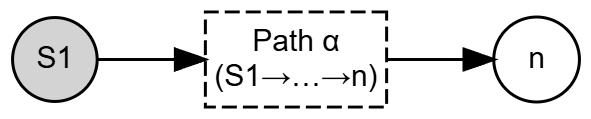
\includegraphics[scale=0.35]{images/chain.png}
  \caption{Single-path structure: chained signal propagation.}
  \label{fig:chain}
\end{figure}

\begin{figure}[htbp]
  \centering
  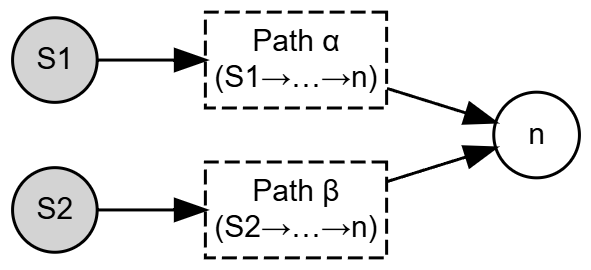
\includegraphics[scale=0.35]{images/indepmulti.png}
  \caption{Multiple independent parent signals: parallel signal propagation.}
  \label{fig:indepmulti}
\end{figure}

\subsubsection{Reconvergent Structures and Independence Breakdown}

The update rule in \eqref{eq:independent_update} is no longer exact when the incoming signal events are dependent. In directed acyclic graphs, this occurs in \emph{reconvergent structures}, where multiple upstream paths share common components before merging at a downstream node.

Let $v$ be a join node receiving signals from parents $\{p_1,p_2\}$. If the upstream paths leading to $p_1$ and $p_2$ share a common ancestor $f$, then the events $A_1$ and $A_2$ are dependent. In that case, applying the independence-based rule
\begin{equation}
P(A_1 \cup A_2) = 1-(1-S_1)(1-S_2)
\label{eq:wrong_indep_formula}
\end{equation}
overestimates the true probability of signal reception, because it ignores the correlation induced by the shared upstream components.

IPA resolves this problem by identifying such reconvergent structures and conditioning on the shared upstream variables that induce the dependency.

\subsubsection{Diamond Structures and Conditional Decomposition}

The fundamental dependency-inducing pattern considered by IPA is a \emph{diamond structure}: a reconvergent fork--join subgraph in which multiple paths diverge from one or more shared upstream nodes and reconverge at a join node.

Consider a single-fork diamond with fork node $f$ and join node $j$. Let
\[
J = \{\text{a signal reaches } j\}, \qquad
F = \{\text{fork node } f \text{ is operational}\}.
\]
By the law of total probability,
\begin{equation}
P(J) = P(J \mid F)P(F) + P(J \mid \bar{F})P(\bar{F}).
\label{eq:diamond_ltp}
\end{equation}

Conditioning on the state of the fork restores independence among the downstream paths:
\begin{itemize}
    \item if $F=1$, the fork is active and the paths downstream of $f$ become conditionally independent;
    \item if $F=0$, no signal can propagate through paths originating from $f$.
\end{itemize}

Thus, if the diamond contains $k$ downstream paths from $f$ to $j$, then
\begin{equation}
P(J \mid F) = 1-\prod_{i=1}^{k}\left(1-S_i^{(F)}\right),
\label{eq:diamond_conditional_update}
\end{equation}
where $S_i^{(F)}$ denotes the probability that path $i$ transmits a signal to $j$ given that the fork is active.

For a simple induced diamond with no alternative upstream routes to the join node,
\begin{equation}
P(J \mid \bar{F}) = 0.
\label{eq:diamond_no_alternative}
\end{equation}

\subsubsection{Generalisation to Multiple Conditioning Nodes}

More complex reconvergent structures may involve several shared upstream nodes
\[
\mathcal{C} = \{c_1,c_2,\ldots,c_m\}.
\]
In that case, the join-node signal probability is computed by enumerating all conditioning states:
\begin{equation}
P(J) = \sum_{s \in \{0,1\}^{m}} P(J \mid s)\,P(s),
\label{eq:multi_conditioning}
\end{equation}
where $s=(s_1,\ldots,s_m)$ is a binary assignment to the conditioning nodes and
\begin{equation}
P(s)=\prod_{i=1}^{m}[b(c_i)]^{s_i}[1-b(c_i)]^{1-s_i}.
\label{eq:state_probability}
\end{equation}

For each conditioning state $s$, the remaining incoming paths to the join node become conditionally independent, so the local update can again be evaluated using the independent-signal formula.

\subsection{Simple Example}\DIFaddbegin \label{sec:simple_example}
\DIFaddend 

To illustrate the effect of reconvergent dependencies and the correctness of the conditioning approach, consider the simple diamond in Figure~\ref{fig:numerical-diamond}. The subgraph consists of a single fork--join pair connected by two intermediate paths. All non-source nodes have intrinsic reliability $0.9$, and all edges have transmission probability $0.9$.

\begin{figure}[htbp]
\centering
  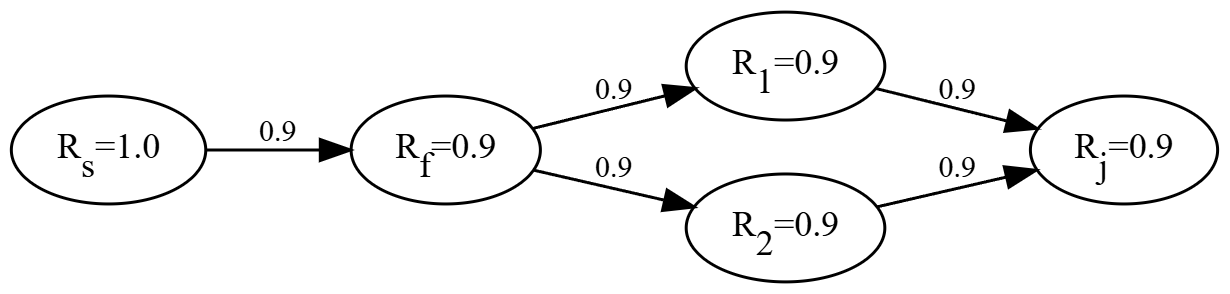
\includegraphics[scale=0.3]{images/numerical-diamond.png}
\caption{A simple diamond subgraph between fork node $f$ and join node $j$.}
\label{fig:numerical-diamond}
\end{figure}

\subsubsection{Solution by Path Enumeration (Correct but Expensive)}

We enumerate the relevant fork/intermediate-node states:
\begin{align*}
P_1 &= 0.81 \times 0.81 \times 0.81 = 0.531441 
    && \text{(fork active, both intermediates work)}, \\
P_2 &= 0.81 \times 0.81 \times 0.19 = 0.124659
    && \text{(fork active, only first intermediate works)}, \\
P_3 &= 0.81 \times 0.19 \times 0.81 = 0.124659
    && \text{(fork active, only second intermediate works)}, \\
P_4 &= 0.81 \times 0.19 \times 0.19 = 0.029241
    && \text{(fork active, both intermediates fail)}, \\
P_5 &= 0.19
    && \text{(fork inactive, no signal possible)}.
\end{align*}

The signal-reception probabilities at the join node are
\[
P(\text{signal}) =
\begin{cases}
0.99, & \text{if both paths send signals}, \\
0.9,  & \text{if only one path sends a signal}, \\
0,    & \text{if no path sends a signal}.
\end{cases}
\]

Hence,
\begin{align*}
P(\text{signal})
&= P_1 \times 0.99 + P_2 \times 0.9 + P_3 \times 0.9 \\
&= 0.531441 \times 0.99 + 0.124659 \times 0.9 + 0.124659 \times 0.9 \\
&= 0.75051279.
\end{align*}
The resulting reliability at the join node is
\[
b(j)=R(j)\,P(\text{signal})=0.9 \times 0.75051279 = 0.675461511.
\]

\subsubsection{Solution by Independent Update (Incorrect)}

Using the independent-parent update yields
\begin{align*}
b(f) &= R(s)\,P(s,f)\,R(f) = 1.0 \times 0.9 \times 0.9 = 0.81, \\
b(p_1)=b(p_2) &= b(f)\,P(f,p)\,R(p) = 0.81 \times 0.9 \times 0.9 = 0.6561.
\end{align*}
Thus,
\[
S_1 = S_2 = b(p_i)\,P(p_i,j) = 0.6561 \times 0.9 = 0.59049.
\]
Treating the two incoming signals as independent gives
\begin{align*}
P(\text{signal}) &= 1-(1-0.59049)^2 = \DIFdelbegin \DIFdel{0.83227}\DIFdelend \DIFaddbegin \DIFadd{0.83230}\DIFaddend , \\
b(j) &= 0.9 \times \DIFdelbegin \DIFdel{0.83227 }\DIFdelend \DIFaddbegin \DIFadd{0.83230 }\DIFaddend = \DIFdelbegin \DIFdel{0.749043}\DIFdelend \DIFaddbegin \DIFadd{0.749071}\DIFaddend ,
\end{align*}
which overestimates the correct value.

\subsubsection{Solution by Diamond Conditioning (Correct and Efficient)}

Conditioning on the fork state, we have
\[
b(f)=0.81.
\]
If the fork is active, each downstream path has conditional transmission probability
\[
P(f,p)\,R(p)\,P(p,j)=0.9 \times 0.9 \times 0.9 = 0.729.
\]
Therefore,
\begin{align*}
P(\text{signal}\mid F=1) &= 1-(1-0.729)^2 = 0.926559, \\
P(\text{signal}\mid F=0) &= 0.
\end{align*}
Using \eqref{eq:diamond_ltp},
\begin{align*}
P(\text{signal})
&= P(\text{signal}\mid F=1)P(F=1) + P(\text{signal}\mid F=0)P(F=0) \\
&= 0.926559 \times 0.81 + 0 \times 0.19 \\
&= 0.75051279.
\end{align*}
Hence,
\[
b(j)=0.9 \times 0.75051279 = 0.675461511,
\]
which matches the exact path-enumeration result.

This example shows the central idea behind IPA: the dependence induced by a reconvergent structure can be handled exactly by conditioning only on the shared upstream variables that generate the dependence.

\subsection{IPA Workflow and \DIFdelbegin \DIFdel{algorithm}\DIFdelend \DIFaddbegin \DIFadd{Algorithm}\DIFaddend }

The Information Propagation Algorithm computes node reliability in a single forward pass over the DAG. For each node, the algorithm:
\begin{itemize}
    \item computes incoming signal probabilities from its parent nodes;
    \item applies the closed-form independent update when the parent signals are independent;
    \item detects reconvergent structures when dependencies are present;
    \item resolves those dependencies through conditional enumeration on shared upstream nodes.
\end{itemize}

This formulation localises exact dependency handling to the subgraphs that require it\DIFdelbegin \DIFdel{, while retaining }\DIFdelend \DIFaddbegin \DIFadd{. Elsewhere, it retains the }\DIFaddend simple closed-form updates\DIFdelbegin \DIFdel{elsewhere}\DIFdelend .

Algorithm~\ref{alg:ipa} summarises the overall \DIFdelbegin \DIFdel{IPA procedure}\DIFdelend \DIFaddbegin \DIFadd{computation}\DIFaddend .

\begin{algorithm}[h]
\caption{Information Propagation Algorithm (IPA)}
\label{alg:ipa}
\begin{algorithmic}[1]
\STATE Compute a topological ordering of $G$
\FOR{each node $v \in V$ in topological order}
    \IF{$v \in S$}
        \STATE $b(v) \gets R(v)$
    \ELSE
        \STATE Compute $S_i = b(p_i)\,P(p_i,v)$ for all $p_i \in \text{Pa}(v)$
        \IF{incoming parent signals are independent}
            \STATE $b(v) \gets R(v)\left[1-\prod_i (1-S_i)\right]$
        \ELSE
            \STATE Identify reconvergent (diamond) structures affecting $v$
            \STATE Resolve dependencies by conditional enumeration
            \STATE Compute $b(v)$ from the conditioned signal probabilities
        \ENDIF
    \ENDIF
\ENDFOR
\RETURN $\{b(v)\}_{v \in V}$
\end{algorithmic}
\end{algorithm}

\subsubsection{Computational Characteristics}

For nodes with independent parent signals, the update cost is $O(|\text{Pa}(v)|)$, so the total computational cost is linear in the number of edges for tree-structured networks.

For nodes involved in reconvergent structures, additional cost arises from conditional enumeration over shared upstream components. If a diamond requires conditioning on $c$ shared upstream variables, the local cost scales as $O(2^c)$\DIFdelbegin \DIFdel{rather than with }\DIFdelend \DIFaddbegin \DIFadd{, independent of }\DIFaddend the total number of full path combinations. The practical efficiency of IPA therefore depends primarily on the number and nesting depth of such dependency-inducing structures.

The next section introduces a progressive decomposition strategy that reduces repeated conditioning by replacing resolved diamond subgraphs with statistically equivalent supernodes.


\section{Progressive Decomposition of Diamond Structures}\DIFdelbegin \DIFdel{Progressive decomposition is the mechanism that makes }\DIFdelend \DIFaddbegin \label{sec:decomp}
\DIFadd{Progressive decomposition aims to make }\DIFaddend IPA practical on \DIFdelbegin \DIFdel{many }\DIFdelend non-trivial DAGs with reconvergent structure. \DIFdelbegin \DIFdel{It preserves exactness by }\DIFdelend \DIFaddbegin \DIFadd{By }\DIFaddend replacing resolved diamonds with conditionally equivalent supernodes, \DIFdelbegin \DIFdel{and it improves efficiency by preventing }\DIFdelend \DIFaddbegin \DIFadd{it preserves exactness and improves efficiency: }\DIFaddend the same dependencies \DIFdelbegin \DIFdel{from being }\DIFdelend \DIFaddbegin \DIFadd{are never }\DIFaddend conditioned on repeatedly.

\DIFdelbegin \DIFdel{While conditional decomposition resolves dependencies locally, real }\DIFdelend \DIFaddbegin \DIFadd{Real }\DIFaddend process networks rarely contain only isolated diamonds. \DIFdelbegin \DIFdel{In practical directed acyclic graphs, reconvergent }\DIFdelend \DIFaddbegin \DIFadd{Reconvergent }\DIFaddend structures often overlap or nest within one another, so that the output of one diamond becomes part of a larger downstream reconvergent structure. \DIFdelbegin \DIFdel{In such cases, repeatedly }\DIFdelend \DIFaddbegin \DIFadd{Repeatedly }\DIFaddend conditioning on the same upstream variables \DIFdelbegin \DIFdel{can lead to severe computational redundancy.
}%DIFDELCMD < 

%DIFDELCMD < %%%
\DIFdel{IPA addresses this issue through }\emph{\DIFdel{progressive diamond decomposition}}%DIFAUXCMD
\DIFdel{. Once a diamond subgraph has been solved, it is replaced by a statistically equivalent }\emph{\DIFdel{supernode}} %DIFAUXCMD
\DIFdel{that preserves its exact conditional behaviour while simplifying the remaining graph. This reduces repeated conditioning over already-resolved substructures and allows nested reconvergent patterns to be handled incrementally.
}%DIFDELCMD < 

%DIFDELCMD < %%%
\DIFdel{Consider a nested reconvergent network in which an inner diamond appears as part of a path in a larger outer diamond. Without decomposition, the inner structure would need to be re-evaluated each time the outer diamond is conditioned on a new upstream state. If the outer and inner diamonds contain multiple conditioning variables, the resulting enumeration cost grows multiplicatively.
}%DIFDELCMD < 

%DIFDELCMD < %%%
\DIFdel{More generally, }\DIFdelend \DIFaddbegin \DIFadd{here causes computational redundancy: }\DIFaddend for a network with $L$ nested dependency levels, a direct conditional evaluation may require
\begin{align}
b(j) = & R(j) \cdot
\sum_{s_1 \in \{0,1\}^{m_1}}
\sum_{s_2 \in \{0,1\}^{m_2}}
\cdots \nonumber \\
&
\sum_{s_L \in \{0,1\}^{m_L}}
P(s_1)P(s_2\mid s_1)\cdots P(s_L\mid s_1,\ldots,s_{L-1})
\,\phi(s_1,\ldots,s_L),
\label{eq:nested_direct_enum}
\end{align}
where $m_\ell$ is the number of conditioning nodes introduced at nesting level $\ell$, and $\phi(\cdot)$ is the resulting signal probability at the join node. \DIFdelbegin \DIFdel{This cost }\DIFdelend \DIFaddbegin \DIFadd{The cost of this direct evaluation }\DIFaddend grows exponentially with both the number of conditioning variables and the depth of nesting. \DIFdelbegin %DIFDELCMD < 

%DIFDELCMD < %%%
\DIFdel{The purpose of progressive decomposition is to avoid this }\DIFdelend \DIFaddbegin \DIFadd{Progressive decomposition avoids the }\DIFaddend repeated re-evaluation \DIFdelbegin \DIFdel{by solving inner diamonds }\DIFdelend \DIFaddbegin \DIFadd{behind \eqref{eq:nested_direct_enum} by solving each diamond }\DIFaddend once, storing \DIFdelbegin \DIFdel{their }\DIFdelend \DIFaddbegin \DIFadd{its }\DIFaddend exact conditional behaviour \DIFaddbegin \DIFadd{in a }\emph{\DIFadd{supernode}}\DIFaddend , and reusing that \DIFdelbegin \DIFdel{information }\DIFdelend \DIFaddbegin \DIFadd{behaviour }\DIFaddend whenever the reduced network is evaluated further downstream.

\subsection{Supernode Representation \DIFaddbegin \DIFadd{and Exactness Guarantees}\DIFaddend }\DIFaddbegin \label{sec:supernode}
\DIFaddend 

Let $D$ be a diamond subgraph with fork-side conditioning set
\[
\mathcal{C}_D = \{c_1,\ldots,c_m\}
\]
and join node $j_D$. Solving the diamond yields the exact conditional signal probability at the join node for every configuration of the conditioning variables:
\begin{equation}
\psi_D(s) = P(J_D \mid s),
\qquad s \in \{0,1\}^{m},
\label{eq:supernode_conditional_map}
\end{equation}
where $J_D$ denotes the event that a signal reaches the join node of the diamond and $s$ is a binary state assignment to $\mathcal{C}_D$. \DIFdelbegin %DIFDELCMD < 

%DIFDELCMD < %%%
\DIFdelend The resolved diamond is then replaced by a supernode that stores the map \DIFdelbegin \[
\DIFdel{s \mapsto \psi_D(s).
}\]%DIFAUXCMD
\DIFdel{This supernode acts as a statistically equivalent component in the reduced graph}\DIFdelend \DIFaddbegin \DIFadd{$s \mapsto \psi_D(s)$}\DIFaddend : whenever the conditioning state $s$ is encountered in a larger downstream computation, the contribution of the original diamond is recovered exactly through \eqref{eq:supernode_conditional_map}, without re-solving the full subgraph. \DIFaddbegin \DIFadd{The following four results make this exact, in order: that a resolved diamond's conditional map does not depend on the outer context it sits in; that conditioning on a shared fork is what makes the map well defined; that independent reconvergent structures at the same join can each be resolved on its own separating set, without joint conditioning over the combined ancestry; and that the supernode replacement is therefore lossless downstream.
}\DIFaddend 

%DIF < The key observation enabling decomposition is that once a diamond has been conditioned on the variables responsible for its internal dependencies, its downstream behaviour is fully characterised by its conditional signal map. This gives rise to the following invariance property.
\DIFdelbegin %DIFDELCMD < 

%DIFDELCMD < \begin{lemma}[Conditional Invariance of a Resolved Diamond]
%DIFDELCMD < %%%
\DIFdel{Let $D_{\mathrm{in}}$ }\DIFdelend \DIFaddbegin \begin{lemma}[Conditional Invariance]\label{lem:invariance}
\DIFadd{Let $D$ }\DIFaddend be a diamond subgraph \DIFdelbegin \DIFdel{embedded within a larger DAG}\DIFdelend \DIFaddbegin \DIFadd{with join $j_D$ and conditioning set $C \subseteq \mathcal{C}_D$}\DIFaddend , and let \DIFdelbegin \DIFdel{$\mathcal{C}_{\mathrm{in}}$ be the conditioning variables required to resolve all dependencies internal to $D_{\mathrm{in}}$. Then the conditional signal probability
}\begin{displaymath}
    \DIFdel{\psi_{D_{\mathrm{in}}}(s) = P(J_{\mathrm{in}} \mid s),
\qquad s \in \{0,1\}^{|\mathcal{C}_{\mathrm{in}}|},
}\end{displaymath}%DIFAUXCMD
\DIFdel{depends only on the internal structure of $D_{\mathrm{in}}$ and the state assignment $s$, and is invariant to any outer conditioningcontext that does not alter the internal topology or component probabilities of $D_{\mathrm{in}}$}\DIFdelend \DIFaddbegin \DIFadd{$\psi_D(s) = P(\mathcal{R}_{j_D}=1 \mid \mathcal{R}_C = s)$, $s \in \{0,1\}^{|C|}$, be its conditional signal map. If an enclosing computation conditions on further variables $A$ disjoint from the nodes and edges internal to $D$, then $\psi_D(s)$ is unchanged by that outer conditioning}\DIFaddend .
\end{lemma}

\begin{proof}
\DIFdelbegin \DIFdel{By construction, all statistical dependencies internal to $D_{\mathrm{in}}$ are removed once }\DIFdelend \DIFaddbegin \DIFadd{Fix $s$. Conditional on $\mathcal{R}_C=s$, the event $\{\mathcal{R}_{j_D}=1\}$ is a deterministic function, by \eqref{eq:reach_indicator}, of the node and edge indicators internal to $D$. By Assumption~\ref{as:indep} these indicators are independent of every indicator outside $D$, in particular of }\DIFaddend the variables in \DIFdelbegin \DIFdel{$\mathcal{C}_{\mathrm{in}}$ are fixed. For any fixed state }\DIFdelend \DIFaddbegin \DIFadd{$A$. Hence $P(\mathcal{R}_{j_D}=1\mid \mathcal{R}_C=s,\mathcal{R}_A=a)=\psi_D(s)$ for every outer state $a$: the outer conditioning changes only the probability with which a state }\DIFaddend $s$ \DIFdelbegin \DIFdel{, the remaining signal probability at the join node is determined solely by the nodes, edges, }\DIFdelend \DIFaddbegin \DIFadd{occurs, never the value $\psi_D(s)$ itself.
}\end{proof}

\DIFadd{The disjointness required by Lemma~\ref{lem:invariance} is what identification enforces (Section~\ref{sec:identification}): whenever an outer state does fix a variable internal to a previously resolved diamond, the sub-problem it defines is a different one and is resolved, and stored, separately.
}

\begin{lemma}[Separator Sufficiency]\label{lem:separator}
\DIFadd{Let $v$ be a join node and let $C \subseteq F \cap \mathrm{anc}(v)$ be a set of forks such that $\mathrm{infl}(u;C)\cap\mathrm{infl}(u';C)=\emptyset$ for every pair of distinct parents $u,u'\in\mathrm{Pa}(v)$, where $\mathrm{infl}$ is defined in \eqref{eq:infl}. Then, conditional on $\mathcal{R}_C$, the parent reachability events $\{\mathcal{R}_u\}_{u\in\mathrm{Pa}(v)}$ are mutually independent, }\DIFaddend and
\DIFdelbegin \DIFdel{path structurecontained within $D_{\mathrm{in}}$.
Any outer conditioning context may affect the probability with which a state $s$ occurs, but it does not change the value of $P(J_{\mathrm{in}} \mid s)$ itself, provided the internal structure and
local probabilities of $D_{\mathrm{in}}$ remain unchanged.
}\DIFdelend \DIFaddbegin \begin{equation}
\DIFadd{b(v\mid \mathcal{R}_C=s) = R(v)\left(1-\prod_{u\in\mathrm{Pa}(v)}\bigl(1-P(\mathcal{R}_u=1\mid \mathcal{R}_C=s)\,P(u,v)\bigr)\right).
}\end{equation}
\end{lemma}

\begin{proof}
\DIFadd{With $\mathcal{R}_C$ fixed, each $\mathcal{R}_u$ is, by \eqref{eq:reach_indicator}, a function of the indicators in $\mathrm{infl}(u;C)$ alone. These sets are disjoint across parents by hypothesis, and functions of disjoint sets of mutually independent indicators (Assumption~\ref{as:indep}) are themselves independent. The stated update is then \eqref{eq:independent_update} applied conditionally on $\mathcal{R}_C=s$.
}\DIFaddend \end{proof}

\DIFdelbegin \DIFdel{This immediately justifies replacement by a supernode. }\DIFdelend \DIFaddbegin \DIFadd{Lemma~\ref{lem:separator} is what the unresolved-influence test of \eqref{eq:infl} is for: identification returns, for each reconvergent structure, a conditioning set with this separating property, so the resulting cost is $2^{|C|}$.
}\DIFaddend 

\DIFaddbegin \begin{lemma}[Independent-Substructure Factorisation]\label{lem:factorisation}
\DIFadd{Fix a conditioning context $E$ and write $u\sim u'$ for parents $u,u'$ of a join $v$ whenever $\mathrm{infl}(u;E)\cap\mathrm{infl}(u';E)\neq\emptyset$. Let $G_1,\ldots,G_m$ be the equivalence classes of $\mathrm{Pa}(v)$ under the transitive closure of $\sim$. The events $\{v\text{ is reached through some parent in }G_k\}$, $k=1,\ldots,m$, are mutually independent, and
}\begin{equation}
\DIFadd{b(v) = R(v)\left(1-\prod_{k=1}^{m}\bigl(1-P(v\text{ reached via }G_k)\bigr)\right),
}\end{equation}
\DIFadd{so each group $G_k$ can be resolved on its own separating set $C_k$ (Lemma~\ref{lem:separator}) independently of the others.
}\end{lemma}

\begin{proof}
\DIFadd{Distinct classes have disjoint unresolved influence by construction, so the class events are functions of disjoint sets of mutually independent indicators, hence independent by Assumption~\ref{as:indep}; the product form is \eqref{eq:independent_update} applied to the $m$ group events.
}\end{proof}

\DIFadd{At a join whose parents form $m$ independent groups with conditioning sets $C_1,\ldots,C_m$, joint conditioning over the combined shared ancestry would enumerate $2^{|C_1|+\cdots+|C_m|}$ states. Lemma~\ref{lem:factorisation} enumerates $\sum_{k=1}^m 2^{|C_k|}$ states instead. For $k$ parents each depending on its own independent fork, this reduces the cost from $2^k$ to $2k$, from exponential to linear in the fan-in.
}

\DIFaddend \begin{lemma}[Supernode Equivalence]\DIFaddbegin \label{lem:supernode}
\DIFaddend Let $D$ be a resolved diamond\DIFaddbegin \DIFadd{, or a resolved independent group $G_k$ of Lemma~\ref{lem:factorisation}, }\DIFaddend with conditional signal map $\psi_D(s)$. Replacing $D$ by a supernode storing $\psi_D(s)$ preserves the exact source-to-node reliability of every downstream node in the reduced graph.
\end{lemma}

\begin{proof}
\DIFdelbegin \DIFdel{For any downstream computation, the }\DIFdelend \DIFaddbegin \DIFadd{The }\DIFaddend contribution of $D$ \DIFaddbegin \DIFadd{to any downstream computation }\DIFaddend enters only through the probability that its join \DIFdelbegin \DIFdel{node }\DIFdelend receives a signal under a given conditioning state. By Lemma\DIFdelbegin \DIFdel{1, this contribution is exactly }\DIFdelend \DIFaddbegin \DIFadd{~\ref{lem:invariance} the stored map equals }\DIFaddend $\psi_D(s)$ \DIFdelbegin \DIFdel{for each state $s$.
Replacing the original diamond by a supernode that returns the same value $\psi_D(s)$ under the same conditioning state therefore leaves all downstream reliability calculations unchanged}\DIFdelend \DIFaddbegin \DIFadd{in every outer context that fixes no variable internal to $D$, and by Lemmas~\ref{lem:separator} and~\ref{lem:factorisation} the downstream update combines this map with the remaining parent signals through the same independent-union rule used elsewhere in IPA. Both are preserved by the replacement, so every downstream belief is unchanged.
}\end{proof}

\begin{corollary}[Acyclic Reduction]\label{cor:acyclic}
\DIFadd{Replacing a resolved diamond $D$, or a resolved independent group $G_k$, by its supernode preserves the acyclicity of the reduced graph, and this holds under repeated replacement across overlapping and nested diamonds.
}\end{corollary}

\begin{proof}
\DIFadd{The supernode has exactly one outgoing edge, to $D$'s join, and its incoming edges are exactly $D$'s external incoming edges (edges entering $D$ from outside $D$), retained with their original source node and direction; no edge internal to $D$ survives the replacement, and no edge is introduced. The reduced graph is therefore obtained from $G$ by contracting an induced subgraph to a single node along its edges, without reversing or adding any edge. A directed cycle in the reduced graph would need to revisit the supernode, which is only possible by leaving it through its single outgoing edge and returning through one of its incoming edges; tracing that path back through the corresponding nodes and edges of $D$ and the external nodes it passes through yields a directed cycle in $G$, contradicting the acyclicity of $G$ (Assumption 1). This is not order-dependent: whenever a diamond $D'$ resolved later contains an already-placed supernode among its own parents or internal nodes, $D'$'s own incoming and outgoing edges are subject to the same argument, so the property is preserved under repeated replacement across nested and overlapping diamonds}\DIFaddend .
\end{proof}

\subsection{Progressive Decomposition Procedure}\DIFaddbegin \label{sec:procedure}
\DIFaddend 

IPA applies diamond decomposition progressively \DIFdelbegin \DIFdel{during topological evaluation. When the algorithm }\DIFdelend \DIFaddbegin \DIFadd{as it processes the network in topological order. When it }\DIFaddend reaches a join node \DIFdelbegin \DIFdel{involved in a reconvergent structure, it :
}%DIFDELCMD < \begin{enumerate}
%DIFDELCMD <     \item %%%
\DIFdel{identifies the associated diamond subgraph, }%DIFDELCMD < \item %%%
\DIFdel{determines the conditioning variables required to resolve its internal dependencies, }%DIFDELCMD < \item %%%
\DIFdel{computes the }\DIFdelend \DIFaddbegin \DIFadd{whose parent signals are dependent, it partitions the parents into independent groups by testing pairwise intersection of their unresolved influence, \eqref{eq:infl} (Lemma~\ref{lem:factorisation}). For each group it finds the earliest fork common to its members and the subgraph this induces, computes the group's }\DIFaddend conditional signal map \DIFdelbegin \DIFdel{of the join node, }%DIFDELCMD < \item %%%
\DIFdel{replaces the entire resolved diamond }\DIFdelend \DIFaddbegin \DIFadd{by conditioning on that fork (Lemma~\ref{lem:separator}), and replaces the resolved group }\DIFaddend by a supernode in the reduced graph \DIFdelbegin \DIFdel{.
}%DIFDELCMD < \end{enumerate}
%DIFDELCMD < %%%
\DIFdelend \DIFaddbegin \DIFadd{(Lemma~\ref{lem:supernode}). Independent groups then combine by the factorised union rule; a single correlated group with no independent partition reduces exactly to the non-factorised case of Section~\ref{sec:supernode}.
}\DIFaddend 

\DIFdelbegin \DIFdel{This procedure transforms the original DAG into a progressively simpler equivalent DAG.
Inner }\DIFdelend \DIFaddbegin \DIFadd{Unlike the single-fork diamond of Section~\ref{sec:simple_example}, a diamond resolved this way can itself sit inside a larger diamond, so that the graph must be simplified from the inside out: inner }\DIFaddend diamonds are resolved first, \DIFdelbegin \DIFdel{so that larger outer diamonds can }\DIFdelend \DIFaddbegin \DIFadd{and outer diamonds then }\DIFaddend treat them as supernodes \DIFdelbegin \DIFdel{rather than re-evaluating }\DIFdelend \DIFaddbegin \DIFadd{and do not re-evaluate }\DIFaddend their internal paths. \DIFdelbegin %DIFDELCMD < 

%DIFDELCMD < %%%
\DIFdelend Figure~\ref{fig:progressive_decomposition} \DIFdelbegin \DIFdel{illustrates the decomposition of a nested reconvergent network }\DIFdelend \DIFaddbegin \DIFadd{shows this on a network with four such diamonds, some nested inside others}\DIFaddend .

\begin{figure}[p]
\centering
\begin{subfigure}[b]{0.21\textwidth}
    \centering
    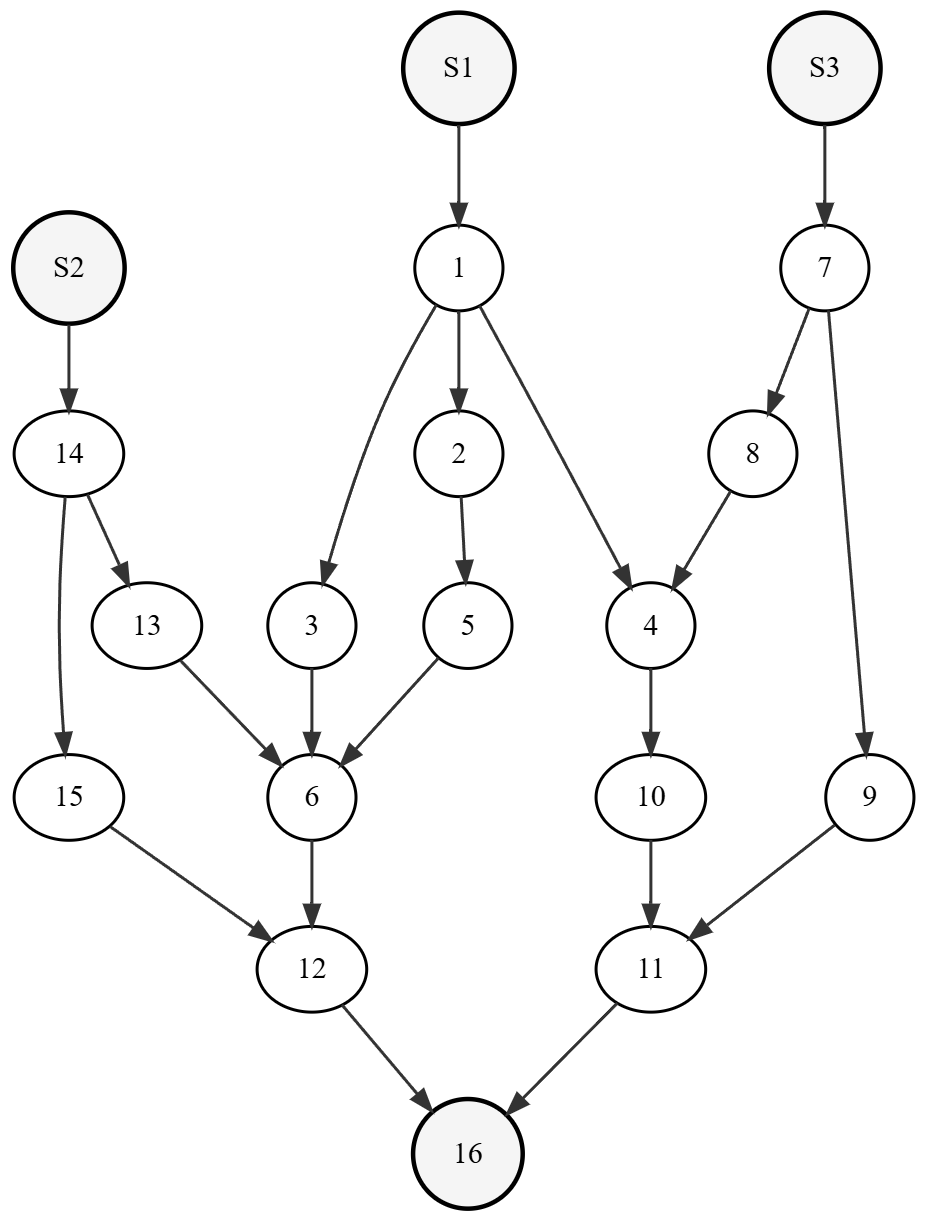
\includegraphics[width=\textwidth]{images/decomp_network/Original Network.png}
    \caption{Original network}
    \label{fig:original}
\end{subfigure}
\quad
\begin{subfigure}[b]{0.21\textwidth}
    \centering
    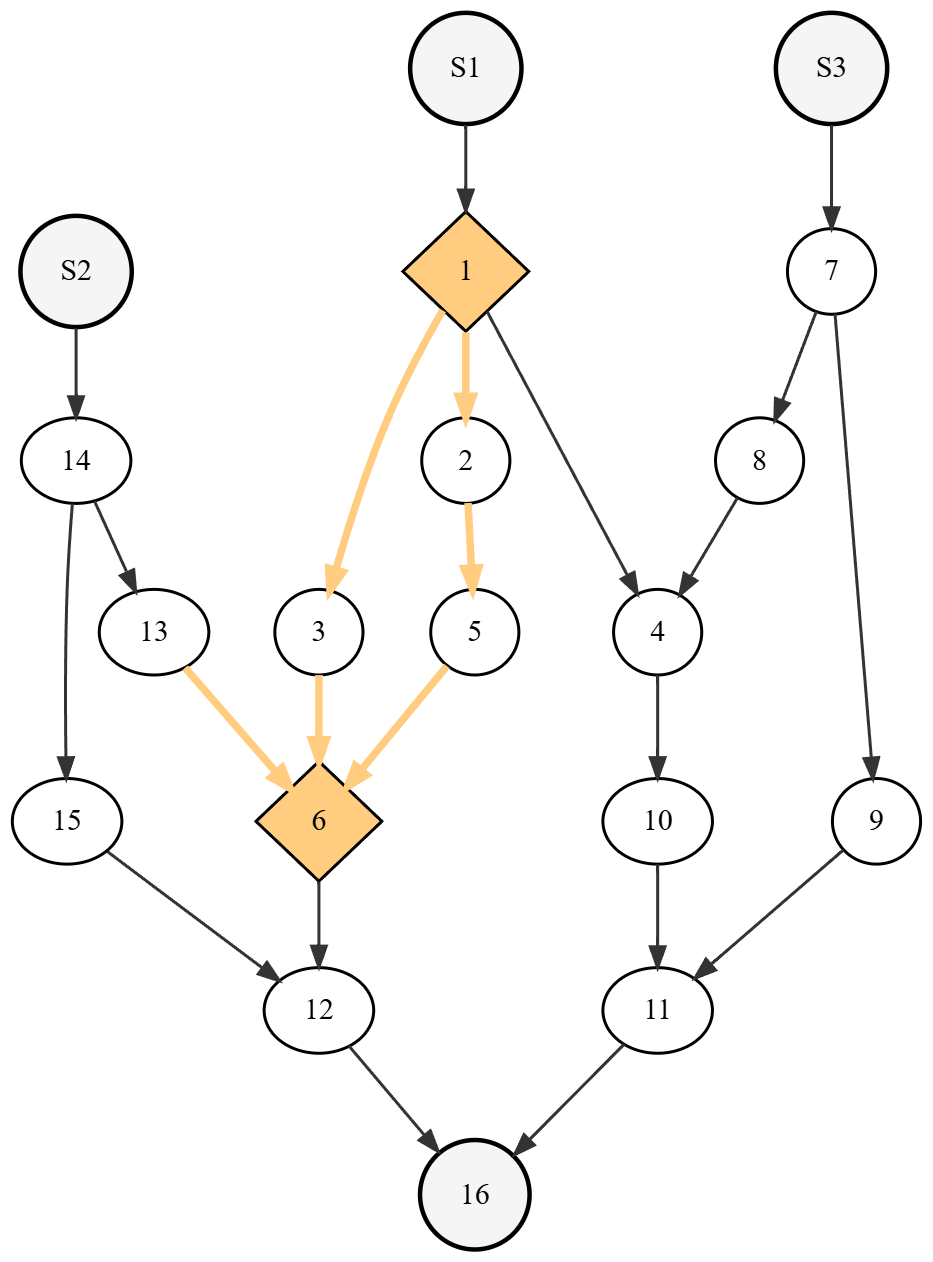
\includegraphics[width=\textwidth]{images/decomp_network/Diamond D1.png}
    \caption{Diamond $D_1$: $1 \rightarrow 6$}
    \label{fig:d1_identify}
\end{subfigure}
\quad
\begin{subfigure}[b]{0.21\textwidth}
    \centering
    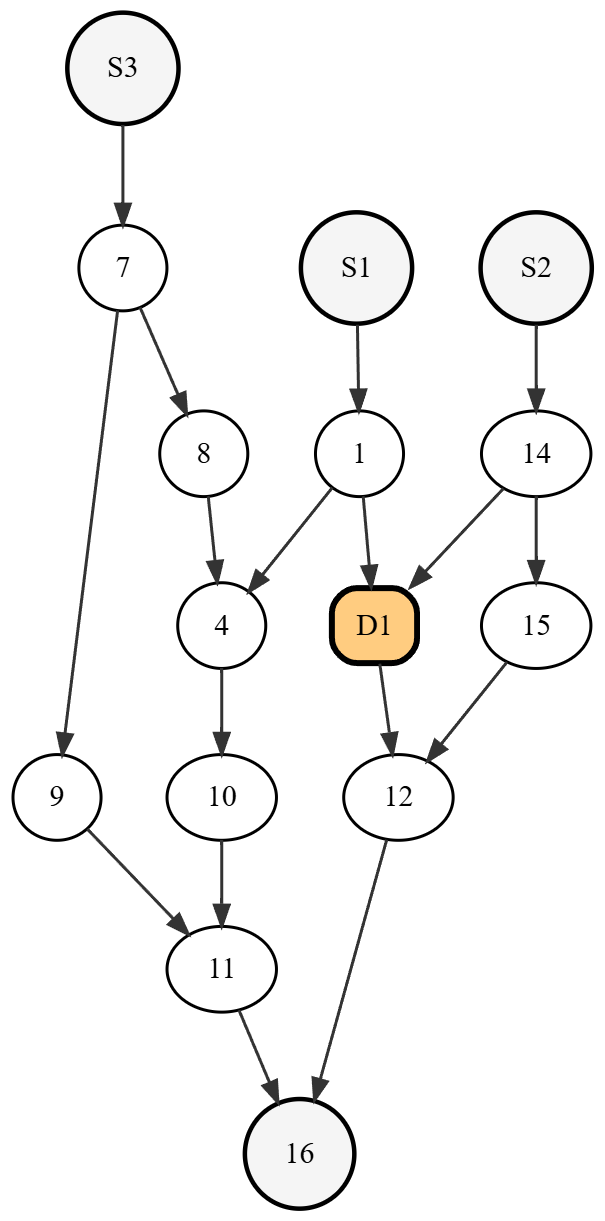
\includegraphics[width=\textwidth]{images/decomp_network/D1 supernode.png}
    \caption{After $D_1$ replacement}
    \label{fig:d1_replace}
\end{subfigure}
\quad
\begin{subfigure}[b]{0.21\textwidth}
    \centering
    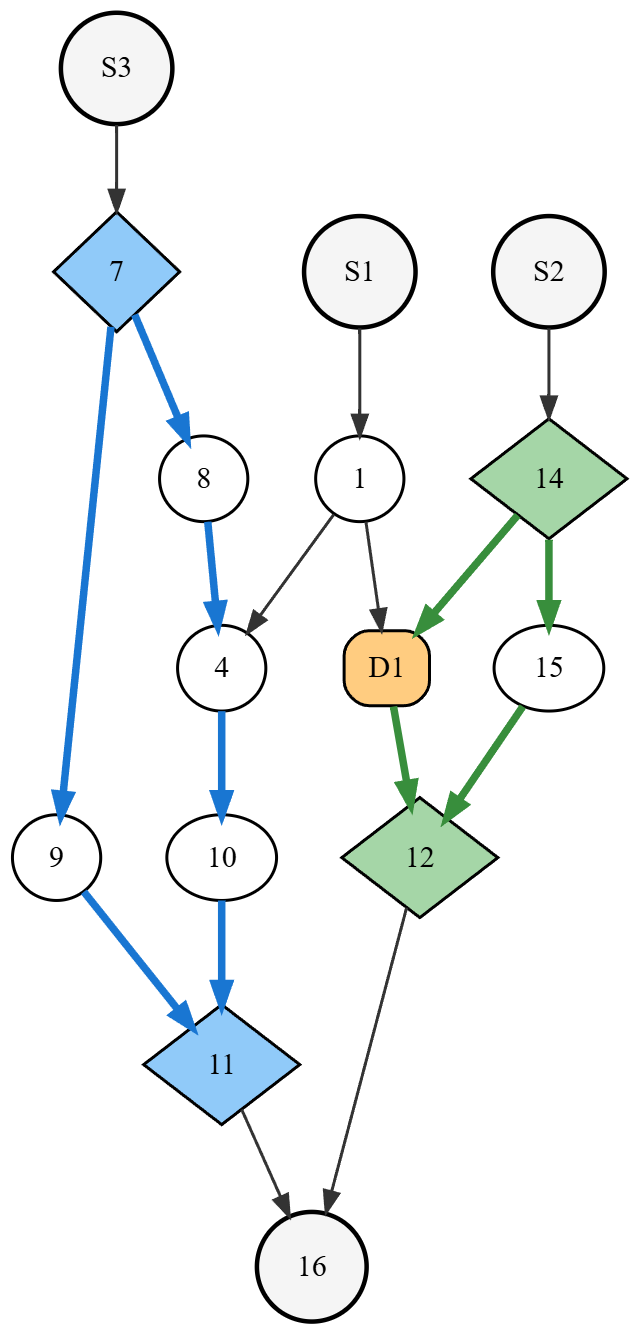
\includegraphics[width=\textwidth]{images/decomp_network/Diamonds D2 and D3.png}
    \caption{Diamonds $D_2$: $7 \rightarrow 11$, $D_3$: $14 \rightarrow 12$}
    \label{fig:d2_d3_identify}
\end{subfigure}

\smallskip

\hspace*{\fill}
\begin{subfigure}[b]{0.25\textwidth}
    \centering
    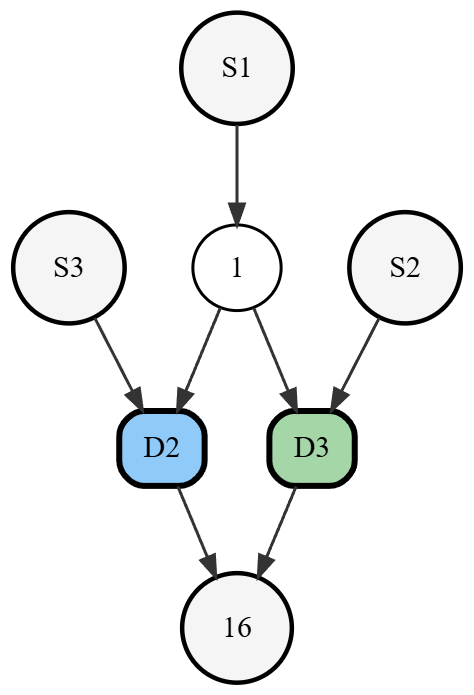
\includegraphics[width=\textwidth]{images/decomp_network/D2 and D3 supernode.png}
    \caption{After $D_2$ and $D_3$ replacement}
    \label{fig:d2_d3_replace}
\end{subfigure}
\hspace*{\fill}
\begin{subfigure}[b]{0.25\textwidth}
    \centering
    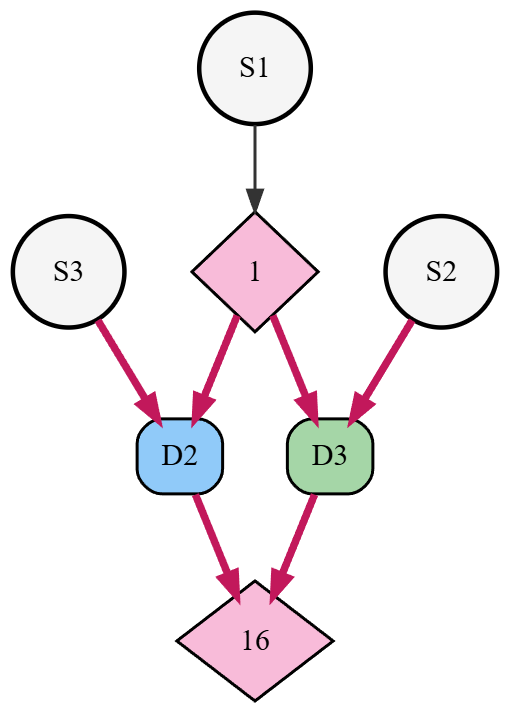
\includegraphics[width=\textwidth]{images/decomp_network/Diamond D4.png}
    \caption{Final diamond $D_4$: $1 \rightarrow 16$}
    \label{fig:d4_identify}
\end{subfigure}
\hspace*{\fill}
\begin{subfigure}[b]{0.25\textwidth}
    \centering
    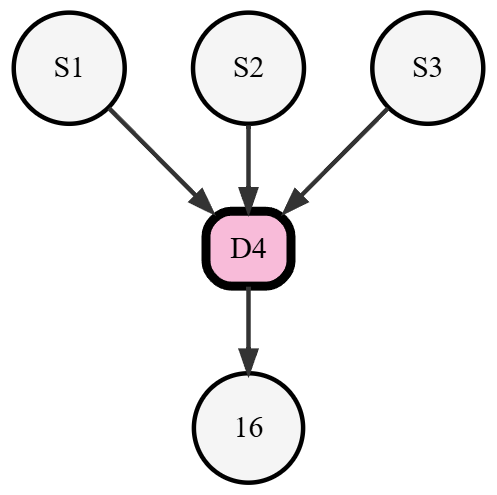
\includegraphics[width=\textwidth]{images/decomp_network/D4 supernode.png}
    \caption{Final decomposition}
    \label{fig:final}
\end{subfigure}
\hspace*{\fill}

\caption{Progressive diamond decomposition in a nested reconvergent network.}
\label{fig:progressive_decomposition}
\end{figure}

\DIFdelbegin \DIFdel{The topological order ensures that the inner }\DIFdelend \DIFaddbegin \subsubsection{\DIFadd{Tracing the example of Figure~\ref{fig:progressive_decomposition}}}\label{sec:worked}

\DIFadd{The network of Figure~\ref{fig:progressive_decomposition} has three sources and sixteen further nodes; every non-source node has intrinsic reliability $0.9$ and every edge has transmission probability $0.9$, as in Section~\ref{sec:simple_example}. Node 6 has three parents, 3, 5, and 13, but only 3 and 5 trace back to the shared fork 1; the third, 13, traces back through node 14 to a different source and carries no dependency on the other two. IPA therefore does not condition node 6 on a joint state of three variables: it resolves $\{3,5\}$ as }\DIFaddend diamond $D_1$ \DIFdelbegin \DIFdel{is detected and resolved before downstream join nodes are processed. Once replaced by a supernode, the reduced graph contains fewer explicit dependency-inducing paths . The same procedure is then applied to }\DIFdelend \DIFaddbegin \DIFadd{(fork 1), then combines the result with node 13's independent signal by the ordinary union rule of Section~\ref{sec:IPA} (Lemma~\ref{lem:factorisation}). Node 4, by contrast, is a join with no diamond at all: its parents 1 and 8 share no common ancestor, so IPA applies the closed-form independent update directly (Section~\ref{sec:IPA}) and never conditions on anything there.
}

\DIFadd{$D_1$ is resolved first, since node 6 is reached before nodes 11, 12, and 16 in topological order. Fork 1 has $b(1)=0.81$; conditional on 1 being reachable, the union of paths through 3 and 5 has probability $\psi_{D_1}(1)=0.8890228$, and conditional on 1 being unreachable no signal can reach 6 through either path, so $\psi_{D_1}(0)=0$. Combining this with node 13's independent signal gives $b(6)=0.7968435$. Diamonds }\DIFaddend $D_2$ \DIFaddbegin \DIFadd{(fork 7, join 11) }\DIFaddend and $D_3$ \DIFaddbegin \DIFadd{(fork 14, join 12) do not depend on $D_1$ or on each other and are resolved the same way, each conditioning on its own fork. The reduced graph then has a single outer diamond}\DIFaddend , \DIFdelbegin \DIFdel{after which the final outer diamond}\DIFdelend $D_4$\DIFdelbegin \DIFdel{can be evaluated using the }\DIFdelend \DIFaddbegin \DIFadd{: fork 1 again, but now covering join 16 through the two }\DIFaddend already-resolved supernodes \DIFaddbegin \DIFadd{at 11 and 12. Fork 1 is conditioned on a second time here, in a different context from $D_1$, and the two resolutions are kept as distinct stored sub-problems (Section~\ref{sec:identification}) because they cover different edges. Table~\ref{tab:worked} lists all four resolutions; the final belief is $b(16)=0.8061491$, and each step was checked independently by exhaustive path enumeration of its own sub-network}\DIFaddend .
\DIFdelbegin \DIFdel{In this way, dependencies are handled locally and only once. }\DIFdelend 

\DIFdelbegin \subsection{\DIFdel{Computational Effect of Decomposition and complexity comparison}}
%DIFAUXCMD
\addtocounter{subsection}{-1}%DIFAUXCMD
\DIFdelend \DIFaddbegin \begin{table}[ht]
\centering\small
\caption{\DIFaddFL{Trace of the four diamond resolutions in Figure~\ref{fig:progressive_decomposition}. $w=P(\mathcal{R}_f{=}1)$; $\psi(1),\psi(0)$ are the conditional signal probabilities at the join given the fork reachable or unreachable, before the join's own reliability is applied.}}
\label{tab:worked}
\begin{tabular}{lcccccc}
\toprule
\DIFaddFL{Diamond }& \DIFaddFL{Join }& \DIFaddFL{Fork }& \DIFaddFL{Group }& \DIFaddFL{$w$ }& \DIFaddFL{$\psi(1)$, $\psi(0)$ }& \DIFaddFL{$b(\text{join})$}\\
\midrule
\DIFaddFL{$D_1$ }& \DIFaddFL{6  }& \DIFaddFL{1 }& \DIFaddFL{\{3,5\} + 13 (indep.) }& \DIFaddFL{0.81 }& \DIFaddFL{0.8890228,\ 0 }& \DIFaddFL{0.7968435}\\
\DIFaddFL{$D_2$ }& \DIFaddFL{11 }& \DIFaddFL{7 }& \DIFaddFL{\{10,9\}              }& \DIFaddFL{0.81 }& \DIFaddFL{0.8937451,\ 0.4782969 }& \DIFaddFL{0.7333289}\\
\DIFaddFL{$D_3$ }& \DIFaddFL{12 }& \DIFaddFL{14 }& \DIFaddFL{\{6,15\}             }& \DIFaddFL{0.81 }& \DIFaddFL{0.9318600,\ 0.5832879 }& \DIFaddFL{0.7790682}\\
\DIFaddFL{$D_4$ }& \DIFaddFL{16 }& \DIFaddFL{1 }& \DIFaddFL{\{12,11\}             }& \DIFaddFL{0.81 }& \DIFaddFL{0.9139431,\ 0.8180383 }& \DIFaddFL{0.8061491}\\
\bottomrule
\end{tabular}
\end{table}
\DIFaddend 

\DIFdelbegin \DIFdel{The benefit of decomposition is not that it removes the exponential nature of exact inference in all cases, but that it prevents repeated enumeration over the same resolved substructures. Without decomposition, nested diamonds may require repeated multi-level conditioning as in \eqref{eq:nested_direct_enum}. With decomposition, }\DIFdelend \DIFaddbegin \subsubsection{\DIFadd{Identification of stored sub-problems}}\label{sec:identification}

\DIFadd{Algorithm~\ref{alg:identify} gives the identification procedure itself, run at each join whose parent signals are dependent. It partitions the join's parents into independent ancestry-groups (Lemma~\ref{lem:factorisation}), finds each group's covering fork, and recurses into nested diamonds under an extended context — this is the recursive partition-and-recurse step that Algorithm~\ref{alg:ipa}'s propagation loop invokes in a single line (``identify reconvergent structures affecting $v$''). A node is excluded from a conditioning set only when it is provably degenerate: fixed at prior exactly $0$, or fixed at exactly $1$ }\emph{\DIFadd{and}} \DIFadd{a graph source. Excluding any other prior-$1$ node is unsound here — it would silently drop a real diamond whenever every prior in the network happens to equal $1$, which is exactly the input convention of the benchmark grid network of Section~\ref{sec:grid}.
}

\begin{algorithm}[h]
\caption{\DIFadd{Diamond identification at a join node (recursive, factorised)}}
\label{alg:identify}
\begin{algorithmic}[1]
\REQUIRE \DIFadd{join node $v$, outer conditioning context $E$ (initially $\emptyset$)
}\ENSURE \DIFadd{independent conditioning groups for $v$, each with its diamond subgraph and conditioning set
}\FOR{each parent $p \in \text{Pa}(v)$}
    \STATE \DIFadd{compute $\text{infl}(p;E) = (\{p\}\cup\text{anc}(p))\setminus E$ }\COMMENT{Eq.~\eqref{eq:infl}}
\ENDFOR
\STATE \DIFadd{partition $\text{Pa}(v)$ into groups $G_1,\ldots,G_m$ by union--find: $p,p'$ share a group iff $\text{infl}(p;E)\cap\text{infl}(p';E)\neq\emptyset$ }\COMMENT{Lemma~\ref{lem:factorisation}}
\FOR{each group $G_k$}
    \STATE \DIFadd{$f_k \gets$ }\DIFaddend the \DIFdelbegin \DIFdel{effective cost is reduced to the accumulation of local conditioning costs over the diamonds that must be resolved}\DIFdelend \DIFaddbegin \DIFadd{topologically-highest fork covering $\geq2$ members of $G_k$ (or the case where one member is an ancestor of another)
    }\IF{no such fork exists}
        \STATE \DIFadd{members of $G_k$ contribute as ordinary non-diamond parents (Section~\ref{sec:IPA})
    }\ELSE
        \STATE \DIFadd{relevant nodes $\gets \{v\}\cup G_k\cup\text{anc}(G_k)$; induced edges $\mathcal{E}_{D_k} \gets$ edges among relevant nodes not crossing into $E$'s already-fixed context
        }\STATE \DIFadd{conditioning set $C_k \gets \{f_k\}\cup(E\cap V(\mathcal{E}_{D_k}))$; key $\gets \mathrm{hkey}(D_k)=(\mathcal{E}_{D_k},C_k)$ }\COMMENT{Eq.~\eqref{eq:hkey}}
        \IF{a diamond with this key is already resolved}
            \STATE \DIFadd{reuse its stored conditional map $\psi_{D_k}$
        }\ELSE
            \STATE \DIFadd{recurse into $D_k$'s own join nodes with context $E\cup\{f_k\}$, then resolve and store $\psi_{D_k}$
        }\ENDIF
    \ENDIF
\ENDFOR
\RETURN \DIFadd{groups $G_1,\ldots,G_m$, each with its conditioning set and conditional map
}\end{algorithmic}
\end{algorithm}

\DIFadd{A resolved diamond is identified for reuse by its edge list together with the conditioning context it was resolved under, not by its edge list alone. The same edge list can arise from a fork that is free or already fixed by an outer context $E$, because cutting the incoming edges of an already-fixed node changes nothing in the induced subgraph; the two occurrences are nonetheless different sub-problems, since Lemma~\ref{lem:invariance} requires the outer context to fix no variable internal to the diamond. IPA keys each stored diamond $D$, with edge list $\mathcal{E}_D$ and covering fork $f$, on
}\begin{equation}
\DIFadd{\mathrm{hkey}(D) = \bigl(\mathcal{E}_D,\ \{f\}\cup(E\cap V(\mathcal{E}_D))\bigr),
\label{eq:hkey}
}\end{equation}
\DIFadd{the edge list together with the new fork and whichever already-fixed forks from the outer context appear among the diamond's own endpoints $V(\mathcal{E}_D)$. Two occurrences of the same edge list under different outer contexts receive different keys and are resolved, and cached, separately; identical sub-problems are resolved once. A conditioning node already fixed by an outer context contributes only one term to the state enumeration of Section~\ref{sec:numerical}, not two, so nesting further levels of context does not double the enumeration already performed at each level.
}

\subsection{\DIFadd{Complexity and Relation to Established Exact Methods}}\label{sec:complexity}

\DIFadd{IPA's cost admits an exact per-instance expression. Let the recursion of Section~\ref{sec:procedure} resolve diamonds $d=1,\ldots,M$, counting nested resolutions, with conditioning sets $C_d$ and internal edge sets $E_d$. The work performed is
}\begin{equation}
\DIFadd{W=\sum_{d=1}^{M}2^{|C_d|}\cdot O(|E_d|),
\label{eq:work}
}\end{equation}
\DIFadd{since each diamond is resolved by enumerating the $2^{|C_d|}$ states of its conditioning set, and each state requires a propagation over the diamond's internal structure. Every term of \eqref{eq:work} is available before enumeration begins, because identification produces the conditioning sets before any state is enumerated; $W$ is a sound a-priori }\emph{\DIFadd{upper bound}} \DIFadd{on the cost of an analysis, computable in advance for a given network. This bound is not the realised cost: memoisation under \eqref{eq:hkey} reduces the work performed to the number of distinct conditional sub-problems encountered. The factorisation of Lemma~\ref{lem:factorisation} reduces the exponents themselves in favourable cases: at a fan-in of $k$ independent branches, from $2^k$ states to a number linear in $k$, without changing the worst-case class}\DIFaddend .

\DIFdelbegin \DIFdel{At a high level, if a nested network contains diamonds $D_1,\ldots,D_M$ with conditioning-set sizes $c_1,\ldots,c_M$, then progressive decomposition avoids repeated multiplicative re-enumeration and replaces it with a }\DIFdelend \DIFaddbegin \paragraph{\DIFadd{Relation to cutset conditioning and junction trees}} \DIFadd{Section~\ref{subsec:relatedworks} positions IPA as a specialisation of cutset conditioning~\mbox{%DIFAUXCMD
\cite{pearl_probabilistic_1988}}\hskip0pt%DIFAUXCMD
. Classical cutset conditioning selects a single global cutset whose state enumeration renders the whole network singly connected, at cost exponential in the cutset size. IPA identifies, at each reconvergence it visits, a local separating set of the parents' shared ancestry (Lemma~\ref{lem:separator}), conditions on it, and recurses, so the realised cost is a }\DIFaddend sum of local \DIFdelbegin \DIFdel{conditional evaluations of order
}\begin{displaymath}
\DIFdel{O\!\left(\sum_{i=1}^{M} 2^{c_i}\right),
\label{eq:decomp_complexity}
}\end{displaymath}%DIFAUXCMD
\DIFdel{provided that previously resolved diamonds can be reused through their stored conditional maps. }\DIFdelend \DIFaddbegin \DIFadd{exponentials, not one global exponential. Tree-structured regions of the network are traversed by the closed-form updates of Section~\ref{sec:IPA} at linear cost, and Lemma~\ref{lem:factorisation} prevents joint conditioning over forks that are independent given the current context. The maximum conditioning-set size on a network is bounded by the size of the largest set of mutually entangled shared ancestors, itself bounded by the treewidth of the network. IPA sits in the same parametric complexity class as the junction-tree algorithm~\mbox{%DIFAUXCMD
\cite{lauritzen_local_1988} }\hskip0pt%DIFAUXCMD
and a well-ordered binary decision diagram: all are exact and fixed-parameter tractable in the relevant width, and none escapes the \#P-hardness of the underlying problem. Section~\ref{sec:comparison} reports a measured comparison of conditioning-set size against decision-diagram size across the validation corpus.
}\DIFaddend 

\DIFdelbegin \DIFdel{This should be interpreted as an }\emph{\DIFdel{effective}} %DIFAUXCMD
\DIFdel{complexity reduction relative to repeated nested conditioning, not as a universal }\DIFdelend \DIFaddbegin \paragraph{\DIFadd{Adversarial structure}} \DIFadd{Two constructed families probe the two ends of this cost. The family $\mathrm{fanin}\text{-}k$ consists of $k$ structurally independent forks that each reconverge, on their own branch, at a single shared join; since no two forks share ancestry, Lemma~\ref{lem:factorisation} conditions each one separately, and identification resolves exactly $2k{+}1$ sub-problems for every $k$ tested. The family $\mathrm{mesh}\text{-}w$ is the opposite extreme: a width-$w$ reconvergent lattice with no independent partition, a single fully correlated block on which factorisation does not apply, so the conditioning-set size and the realised work both grow with $w$. Table~\ref{tab:adversarial} reports both families against an independent decision-diagram method built under dynamic variable reordering: independent structure is resolved at a cost linear in the fan-in, while correlated structure pays the full width-exponential cost of \eqref{eq:work}. A real published benchmark circuit family, assigned the same }\DIFaddend worst-case \DIFdelbegin \DIFdel{bound for all graph topologies. In highly entangled reconvergent networks with many contextual entry points, reuse may be limited and the practical cost may still grow rapidly. }\DIFdelend \DIFaddbegin \DIFadd{input convention, is examined in Section~\ref{sec:adversarial}.
}\DIFaddend 

\DIFdel{Table~\ref{tab:complexity_comparison} summarises the qualitative effect of progressive decomposition on different update types.}

\textcolor{red}{[Table removed: ``Qualitative complexity comparison for node updates with and without progressive decomposition'' --- Update Type / Without Decomposition / With Decomposition, rows: Single parent update ($O(1)$/$O(1)$); Independent multi-parent update ($O(|\mathrm{Pa}(v)|)$/$O(|\mathrm{Pa}(v)|)$); Single diamond with $c$ conditioning nodes ($O(2^c\cdot d)$/$O(2^c)$); Nested diamonds (repeated nested conditioning/accumulated local conditioning). Footnote: ``Here $d$ denotes the size of the diamond subgraph, and $c$ denotes the number of conditioning variables required to resolve its internal dependencies.'']}

\begin{table}[ht]
\small
\caption{\textcolor{blue}{Complexity on the two adversarial families: realised sub-problems for IPA (with factorisation) against a sifted reduced-ordered binary decision diagram, in operation-count and wall-clock terms.}}
\label{tab:adversarial}
\centering
\begin{tabular}{lrrrrr}
\toprule
\textcolor{blue}{Family} & \textcolor{blue}{param} & \textcolor{blue}{IPA sub-problems} & \textcolor{blue}{diagram nodes} & \textcolor{blue}{IPA time} & \textcolor{blue}{diagram time}\\
\midrule
\textcolor{blue}{fan-in-$k$} & \textcolor{blue}{8}  & \textcolor{blue}{17} & \textcolor{blue}{474} & \textcolor{blue}{$<$1\,ms} & \textcolor{blue}{$\sim$1--2\,s}\\
\textcolor{blue}{fan-in-$k$} & \textcolor{blue}{16} & \textcolor{blue}{33} & \textcolor{blue}{802} & \textcolor{blue}{$<$1\,ms} & \textcolor{blue}{$\sim$1--2\,s}\\
\textcolor{blue}{mesh-$w$}   & \textcolor{blue}{4}  & \textcolor{blue}{20{,}603} & \textcolor{blue}{700} & \textcolor{blue}{0.36\,s} & \textcolor{blue}{1.19\,s}\\
\textcolor{blue}{mesh-$w$}   & \textcolor{blue}{5}  & \textcolor{blue}{170{,}001} & \textcolor{blue}{805} & \textcolor{blue}{3.9\,s} & \textcolor{blue}{1.2\,s}\\
\textcolor{blue}{mesh-$w$}   & \textcolor{blue}{8}  & \textcolor{blue}{3{,}895{,}252} & \textcolor{blue}{2{,}621} & \textcolor{blue}{159.5\,s} & \textcolor{blue}{2.9\,s}\\
\textcolor{blue}{mesh-$w$}   & \textcolor{blue}{9}  & \textcolor{blue}{5{,}426{,}417} & \textcolor{blue}{3{,}335} & \textcolor{blue}{5925\,s} & \textcolor{blue}{3.8\,s}\\
\bottomrule
\end{tabular}
\end{table}

\DIFdelbegin \DIFdel{The remaining computational bottleneck of }\DIFdelend \DIFaddbegin \DIFadd{At $w{=}9$ the sub-problem count grows by only $1.39\times$ over $w{=}8$ (3}{\DIFadd{,}}\DIFadd{895}{\DIFadd{,}}\DIFadd{252 to 5}{\DIFadd{,}}\DIFadd{426}{\DIFadd{,}}\DIFadd{417) while IPA's wall-clock time grows by $37\times$ (159.5\,s to 5925\,s); $w{=}10$ exceeded a 180-second-per-step time budget during identification and was not completed. The sub-problem count of \eqref{eq:work} tracks realised work only up to a point: at the largest conditioning-set sizes reached in this family, memory pressure within individual sub-problems begins to dominate wall-clock cost before it is reflected in the sub-problem count itself, and }\DIFaddend the \DIFdelbegin \DIFdel{approach is governed not simply by network size, but by the number, size, and nesting depth of dependency-inducing diamond structures as explored empirically in the case studies that follow}\DIFdelend \DIFaddbegin \DIFadd{decision diagram's wall-clock cost — already lower at every mesh-$w$ point tested — pulls further ahead than the sub-problem-count comparison alone would suggest.
}

\paragraph{\DIFadd{Applicability beyond source-to-node reachability}} \DIFadd{Cutset conditioning already applies to general Bayesian-network inference: IPA specialises that method to source-to-node reachability, and this specialisation does not generalise back to arbitrary probabilistic graphical models. Its closed-form update rules, the independent-union combination of parent signals and the context-keyed supernode cache, are derived for the monotone reachability structure of \eqref{eq:reach_indicator} and do not carry over directly to a Bayesian network with arbitrary conditional probability tables. What transfers is the width-governed complexity class established above. This distinction also bears on the imprecise propagation of Section~\ref{subsec:impreciseinputs}: for classical, precise Bayesian networks, bounded treewidth guarantees polynomial exact inference, but this guarantee does not survive the move to imprecise, credal parameters, where bounded-treewidth inference remains NP-hard in general~\mbox{%DIFAUXCMD
\cite{maua_thirty_2020}}\hskip0pt%DIFAUXCMD
, and the only known tractable relaxation is an approximation scheme; no known exact one exists for that case~\mbox{%DIFAUXCMD
\cite{fagiuoli_2u_1998}}\hskip0pt%DIFAUXCMD
. IPA's width-governed }\emph{\DIFadd{exact}} \DIFadd{imprecise result (Section~\ref{sec:imprecise}) is specific to the monotone arithmetic structure of the reachability problem and the explicit diamond-conditioning construction; it does not imply that general credal-network inference could be made exact at the same cost}\DIFaddend .

\subsection{\DIFdelbegin \DIFdel{Implementation in Julia}\DIFdelend \DIFaddbegin \DIFadd{Numerical Realisation}\DIFaddend }\DIFaddbegin \label{sec:numerical}
\DIFaddend 

IPA is implemented in Julia as \DIFdelbegin \DIFdel{both }\DIFdelend part of the \texttt{InfoPropFramework.jl} package and the standalone library \texttt{InformationPropagationAnalysis.jl}\DIFdelbegin \DIFdel{. In both cases, the algorithm’s functions are exposed in }\DIFdelend \DIFaddbegin \DIFadd{, with diamond identification exposed in }\texttt{\DIFadd{DiamondDecompositionModule}} \DIFadd{and belief propagation in }\DIFaddend \texttt{ProbabilityPropagationModule}\DIFdelbegin \DIFdel{. The module validates network input contracts, then propagates node beliefs from source-to-sink  in topological order, }\DIFdelend \DIFaddbegin \DIFadd{, }\DIFaddend following Section~\ref{sec:IPA} and Algorithm~\ref{alg:ipa}. The propagation flow is type-parametric\DIFdelbegin \DIFdel{:
}\DIFdelend \DIFaddbegin \DIFadd{,
}\DIFaddend \[
T <: \mathrm{Union}\{\texttt{Float64}, \texttt{Interval}, \texttt{pbox}\}\DIFdelbegin \DIFdel{.
}\DIFdelend \DIFaddbegin \DIFadd{,
}\DIFaddend \]
\DIFdelbegin %DIFDELCMD < 

%DIFDELCMD < %%%
\DIFdel{One core engine is }\DIFdelend \DIFaddbegin \DIFadd{with one core engine }\DIFaddend shared across all three \DIFdelbegin \DIFdel{probability representations , with }\DIFdelend \DIFaddbegin \DIFadd{representations and }\DIFaddend type-specific \DIFdelbegin \DIFdel{arithmetic }\DIFdelend dispatch through common \DIFaddbegin \DIFadd{arithmetic }\DIFaddend helpers (addition, multiplication, complement\DIFdelbegin \DIFdel{, subtraction, and product/sum operations}\DIFdelend ).

\DIFdelbegin \DIFdel{For multi-parent updates , }\DIFdelend \DIFaddbegin \DIFadd{Multi-parent updates are evaluated in the product form $1-\prod_i(1-p_i)$. This is equivalent under independence to the alternating }\DIFaddend inclusion--exclusion \DIFdelbegin \DIFdel{is evaluated in product form,
}\[
\DIFdel{1 - \prod_i (1 - p_i),
}\]%DIFAUXCMD
\DIFdel{which is equivalent to the alternating-sum form under independence but is numerically more stable , especially }\DIFdelend \DIFaddbegin \DIFadd{sum, but the product form is numerically stable and avoids the spurious widening the alternating sum introduces }\DIFaddend for interval-valued inputs. \DIFdelbegin %DIFDELCMD < 

%DIFDELCMD < %%%
\DIFdel{At diamond join nodes}\DIFdelend \DIFaddbegin \DIFadd{At a resolved diamond}\DIFaddend , beliefs are computed by enumerating \DIFdelbegin \DIFdel{states of the identified diamond-conditioning set. Each state defines a conditioned subproblem on the corresponding diamondsubgraph, and the join belief is recovered by weighted stateaggregation.
}\DIFdelend \DIFaddbegin \DIFadd{the states of its }\emph{\DIFadd{active}} \DIFadd{conditioning set: a conditioning node whose contextual belief is already pinned to $0$ or $1$ by an outer conditioning contributes only one term, not two, matching \eqref{eq:hkey}'s treatment of already-fixed forks, and never changes the result, since the dropped state carries zero weight. Two caches support this: one keyed on $\mathrm{hkey}(D)$ (Section~\ref{sec:identification}) avoids re-identifying the same diamond, and a second, keyed on a diamond's edge list together with the node priors of a given conditioning state, avoids recomputing a state's belief when the identical sub-problem recurs under a different diamond or context.
}

\DIFaddend For interval inputs, \DIFdelbegin \DIFdel{aggregation uses corner-state evaluation of }\DIFdelend \DIFaddbegin \DIFadd{each conditioning state is evaluated at the corner states of the }\DIFaddend conditioning bounds, \DIFdelbegin \DIFdel{then encloses the result }\DIFdelend \DIFaddbegin \DIFadd{and the result is enclosed }\DIFaddend in an interval envelope\DIFdelbegin \DIFdel{.
}\DIFdelend \DIFaddbegin \DIFadd{; Section~\ref{sec:imprecise} shows this yields the exact range, by the monotonicity of \eqref{eq:reach_indicator}. For probability-box inputs, recombining a diamond's two conditional branches is a convex combination of two dependent random quantities, not an independent sum: a flat weighted sum of the branch distributions, exact for the point-valued and interval cases, is unsound for probability boxes, since it double-counts the shared dependence on the conditioning weight and can return a bound outside $[0,1]$. IPA combines the two branches through the operator of Williamson and Downs~\mbox{%DIFAUXCMD
\cite{williamson_probabilistic_1990}}\hskip0pt%DIFAUXCMD
, nesting one such combination per conditioning node so that $m$ nested two-way combinations reproduce the $2^m$-state mixture exactly.
}\DIFaddend 

\DIFdelbegin \DIFdel{Resolved diamonds (supernodes) are cached as conditional state-to-belief maps and reused as drop-in equivalents in downstream updates. The cache key includes both the diamond subgraph structure and }\DIFdelend \DIFaddbegin \DIFadd{This recursive structure is shared across all three input types: }\DIFaddend the \DIFdelbegin \DIFdel{current prior-state context inside that subgraph.
Supernode reuse is therefore structure-aware }\DIFdelend \DIFaddbegin \DIFadd{number of conditioning states enumerated per diamond, after the memoisation of Section~\ref{sec:identification}, is the same realised-work quantity reported in Section~\ref{sec:complexity}. What differs is the price paid per resolved state. For point-valued and interval inputs this price is $O(1)$; for probability-box inputs, the conditioning weight is represented at a chosen discretisation level, and each combination integrates over that discretisation via the convolution of Williamson and Downs~\mbox{%DIFAUXCMD
\cite{williamson_probabilistic_1990}}\hskip0pt%DIFAUXCMD
, at a cost that increases with the discretisation level. Probability-box cost is therefore governed by the same realised sub-problem count as the exact }\DIFaddend and \DIFdelbegin \DIFdel{state-aware: when the same diamondsubgraph is evaluated under different contextual priors, it is treated as a different cache state. This is most important in nested diamonds, where outer-context beliefs can change the local conditional map even when the internal edge set is unchanged.
}%DIFDELCMD < 

%DIFDELCMD < %%%
\DIFdel{To keep }\texttt{\DIFdel{pbox}} %DIFAUXCMD
\DIFdel{propagation logic aligned with the deterministic and }\DIFdelend interval cases, \DIFdelbegin \DIFdel{the module inherits arithmetic helpers from the Julia library }\texttt{\DIFdel{ProbabilityBoundsAnalysis.jl}}%DIFAUXCMD
\DIFdel{~\mbox{%DIFAUXCMD
\cite{gray_probabilityboundsanalysis}}\hskip0pt%DIFAUXCMD
, which provides independent convolution operators to compute pbox envelope propagation under path dependencies}\DIFdelend \DIFaddbegin \DIFadd{multiplied by a per-state price set by the discretisation level, and Section~\ref{sec:imprecise} reports this cost in those terms, not against network size alone}\DIFaddend .



\clearpage  % Forces all pending floats to be placed
\section{Case Studies}\DIFaddbegin \label{sec:cases}

\DIFaddend This section evaluates IPA in \DIFdelbegin \DIFdel{two complementary settings. The first case study uses a benchmark directed grid network to assess numerical accuracy and computational performance against published results for the directed Probability Propagation Method (dPrPm)~\mbox{%DIFAUXCMD
\cite{tong_probability_2019}}\hskip0pt%DIFAUXCMD
.
The second applies IPA to a set of directed acyclic graphs derived from Pareto-optimal drone logistics networks in order to examine how reconvergent structure and diamond nesting affect the practical tractability of exact reliability analysis in realistic infrastructure systems}\DIFdelend \DIFaddbegin \DIFadd{five parts: a benchmark validation on a grid network (Section~\ref{sec:grid}); a corpus-wide validation and cost comparison against an independent exact decision-diagram method (Section~\ref{sec:comparison}); the imprecise-propagation capability (Section~\ref{sec:imprecise}); an applied case study of a medical drone logistics network for Scotland (Section~\ref{sec:drone}); and a real published benchmark family examined under an adversarial input convention (Section~\ref{sec:adversarial}).
}

\DIFadd{Two methodological points hold throughout the section. Every runtime is measured after a warm-up run of the same computation is executed and discarded, so one-off program-initialisation cost is excluded, and the reported time is the minimum of repeated measurements on otherwise idle hardware. All decision-diagram comparisons use CUDD~\mbox{%DIFAUXCMD
\cite{somenzi_cudd}}\hskip0pt%DIFAUXCMD
, called from the same process and machine as IPA, with dynamic variable reordering enabled unless stated otherwise. Where component reliabilities are widened into intervals or probability boxes for illustration, only components that are not structurally certain are widened: a component fixed at reliability exactly 0 or 1 by the network's own structure is left at that value, since degrading a structural certainty into a synthetic uncertainty would change the problem being analysed}\DIFaddend .

\subsection{Benchmark Validation on a Grid Network}\DIFaddbegin \label{sec:grid}
\DIFaddend 

\subsubsection{Benchmark setup}
\DIFdelbegin \DIFdel{Both the proposed Information Propagation Algorithm (IPA) }\DIFdelend \DIFaddbegin 

\DIFadd{The proposed method }\DIFaddend and Tong and Tien's directed Probability Propagation Method (dPrPm)~\cite{tong_probability_2019} \DIFdelbegin \DIFdel{acompute }\DIFdelend \DIFaddbegin \DIFadd{both compute }\DIFaddend node reliability in directed acyclic networks by propagating local probability information from upstream to downstream nodes\DIFdelbegin \DIFdel{.. Both methods exploit }\DIFdelend \DIFaddbegin \DIFadd{, exploiting }\DIFaddend the acyclic structure \DIFdelbegin \DIFdel{of the graph to ensure }\DIFdelend \DIFaddbegin \DIFadd{so }\DIFaddend that upstream dependencies are processed before downstream updates. \DIFdelbegin %DIFDELCMD < 

%DIFDELCMD < %%%
\DIFdelend The two methods differ in how dependencies are represented\DIFdelbegin \DIFdel{and resolved}\DIFdelend . dPrPm propagates both marginal and pairwise probabilities and \DIFdelbegin \DIFdel{uses local approximations to account for dependent interactions. Specifically, when multiple predecessors influence a node, the update rules explicitly rely on approximating a }\DIFdelend \DIFaddbegin \DIFadd{approximates a }\DIFaddend three-node joint distribution for every \DIFdelbegin \DIFdel{new edge introduced. These rules are fundamental when the incoming messages are combined in an intermediate structure, where the new link addition affects nodes that have already received some information, requiring a more nuanced treatment of shared dependencies. Although effective, this approach requires storing both marginal and }\DIFdelend \DIFaddbegin \DIFadd{edge that introduces a new dependency; this requires storing }\DIFaddend pairwise probabilities throughout the network, which \DIFdelbegin \DIFdel{can become }\DIFdelend \DIFaddbegin \DIFadd{becomes }\DIFaddend memory-intensive in large or dense networks. \DIFdelbegin %DIFDELCMD < 

%DIFDELCMD < %%%
\DIFdel{IPA takes a fundamentally different view of network dependencies by }\DIFdelend \DIFaddbegin \DIFadd{IPA instead }\DIFaddend identifies reconvergent dependency patterns as diamond structures and resolves them through conditional decomposition \DIFdelbegin \DIFdel{.. Rather than tracking pairwise relationships, it identifies and decomposes these structures into statistically equivalent supernodes.  As a result, IPA avoids maintaining or updating pairwise dependencies at complex intersection points, since the relevant }\DIFdelend \DIFaddbegin \DIFadd{(Section~\ref{sec:IPA}). It does not track pairwise relationships: each diamond is decomposed once into a statistically equivalent supernode, and the relevant dependency }\DIFaddend structure is captured \DIFdelbegin \DIFdel{inherently in the decomposition}\DIFdelend \DIFaddbegin \DIFadd{once in that decomposition, not maintained node by node}\DIFaddend .

To provide a direct benchmark, IPA is applied to the same 16-node directed grid network studied in~\cite{tong_probability_2019}, shown in Figure~\ref{fig:grid_network}. This benchmark \DIFdelbegin \DIFdel{is useful because it }\DIFdelend contains multiple reconvergent structures while remaining small enough for exact verification by explicit \DIFdelbegin \DIFdel{path-based computation}\DIFdelend \DIFaddbegin \DIFadd{path enumeration}\DIFaddend . Following~\cite{tong_probability_2019}, all source nodes are assigned prior reliability \DIFdelbegin \DIFdel{1.0 }\DIFdelend \DIFaddbegin \DIFadd{$1.0$ }\DIFaddend and all directed edges are assigned transmission probability \DIFdelbegin \DIFdel{$R_l = 0.9$}\DIFdelend \DIFaddbegin \DIFadd{$0.9$}\DIFaddend .

\begin{figure}[htbp]
\centering
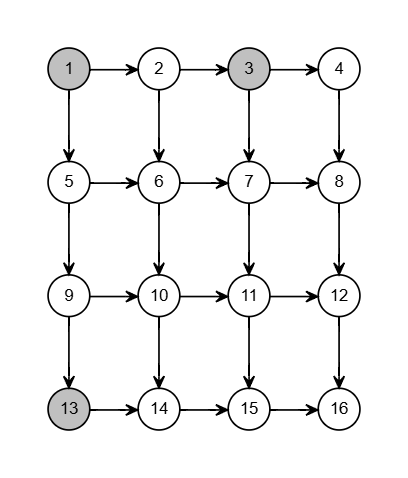
\includegraphics[width=0.8\linewidth, height=8cm]{images/grid_graph.png}
\caption{16-node directed grid network~\cite{tong_probability_2019}. Source nodes 1, 3, and 13 are coloured in grey.}
\label{fig:grid_network}
\end{figure}

\subsubsection{Accuracy results}

Table~\ref{tab:resultcomparison_grid} \DIFdelbegin \DIFdel{compares the nodereliabilities obtained using IPA with exact values and with }\DIFdelend \DIFaddbegin \DIFadd{brings together three independent quantities at every node: the value IPA computes, the value a reduced-ordered binary decision diagram (ROBDD) computes for the same network, and }\DIFaddend the lower and upper bounds \DIFdelbegin \DIFdel{reported }\DIFdelend \DIFaddbegin \DIFadd{published }\DIFaddend for dPrPm in~\cite{tong_probability_2019}. IPA \DIFdelbegin \DIFdel{reproduces the exact values up }\DIFdelend \DIFaddbegin \DIFadd{and the ROBDD agree }\DIFaddend to floating-point precision \DIFdelbegin \DIFdel{. By contrast, dPrPm provides tight lower and upper bounds that coincide with the exact values for many nodes in this }\DIFdelend \DIFaddbegin \DIFadd{at every node, with a worst disagreement of $1.1\times10^{-16}$; the column reported as exact is therefore not IPA's own output taken on trust, but a value two independent exact methods reach separately. Against that value, the dPrPm bounds coincide everywhere except node 16, where a gap of $0.00048$ remains: the same node the source study itself identifies as the lowest-probability, hardest-to-bound event in the }\DIFaddend benchmark.

\begin{table}[!ht]
\centering\DIFaddbeginFL \small
\DIFaddendFL \caption{\DIFdelbeginFL \DIFdelFL{Comparison of node reliability computed for }\DIFdelendFL \DIFaddbeginFL \DIFaddFL{Node reliabilities on }\DIFaddendFL the \DIFaddbeginFL \DIFaddFL{benchmark }\DIFaddendFL grid network (\DIFdelbeginFL \DIFdelFL{$R_l = 0.9$}\DIFdelendFL \DIFaddbeginFL \DIFaddFL{$R_l=0.9$}\DIFaddendFL ). \DIFaddbeginFL \DIFaddFL{The exact column is where IPA and an independent ROBDD agree (worst disagreement $1.1\times10^{-16}$); dPrPm lower/upper bounds and gap are as reported in~\mbox{%DIFAUXCMD
\cite{tong_probability_2019}}\hskip0pt%DIFAUXCMD
, Table 2; the source prints the node-16 gap as $0.00048$, although its printed bounds differ by $0.00052$. Source nodes (1, 3, 13) are fixed at reliability 1 and are not reported as dPrPm bounds in the source study.}\DIFaddendFL }
\label{tab:resultcomparison_grid}
\DIFdelbeginFL %DIFDELCMD < \adjustbox{width=\textwidth,center}{
%DIFDELCMD < \small
%DIFDELCMD < \begin{tabular}{c c c c c c c c c}
%DIFDELCMD < \toprule
%DIFDELCMD < \textbf{Node} & \textbf{Exact} & \textbf{IPA} & \textbf{Abs. Error} & \textbf{Error (\%)} & \textbf{dPrPm (Lower)$^\dagger$} & \textbf{dPrPm (Upper)$^\dagger$} & \textbf{Gap$^\dagger$} & \textbf{dPrPm Error (\%)$^\dagger$} \\
%DIFDELCMD < \midrule
%DIFDELCMD < 1  & 1.00000 & 1.00000 & 0.00000 & 0.00000 & 1.00000 & 1.00000 & 0.00000 & 0.00000 \\
%DIFDELCMD < 2  & 0.99000 & 0.99000 & 0.00000 & 0.00000 & 0.99000 & 0.99000 & 0.00000 & 0.00000 \\
%DIFDELCMD < 3  & 1.00000 & 1.00000 & 0.00000 & 0.00000 & 1.00000 & 1.00000 & 0.00000 & 0.00000 \\
%DIFDELCMD < 4  & 0.98015 & 0.98015 & \num{8.88e-16} & \num{9.06e-14} & 0.98015 & 0.98015 & 0.00000 & 0.00000 \\
%DIFDELCMD < 5  & 0.90000 & 0.90000 & 0.00000 & 0.00000 & 0.90000 & 0.90000 & 0.00000 & 0.00000 \\
%DIFDELCMD < 6  & 0.99510 & 0.99510 & \num{9.99e-16} & \num{1.00e-13} & 0.99510 & 0.99510 & 0.00000 & 0.00000 \\
%DIFDELCMD < 7  & 0.98956 & 0.98956 & \num{4.44e-16} & \num{4.49e-14} & 0.98956 & 0.98956 & 0.00000 & 0.00000 \\
%DIFDELCMD < 8  & 0.89060 & 0.89060 & \num{5.55e-16} & \num{6.23e-14} & 0.89060 & 0.89060 & 0.00000 & 0.00000 \\
%DIFDELCMD < 9  & 0.98100 & 0.98100 & 0.00000 & 0.00000 & 0.98100 & 0.98100 & 0.00000 & 0.00000 \\
%DIFDELCMD < 10 & 0.88290 & 0.88290 & \num{1.11e-16} & \num{1.26e-14} & 0.88290 & 0.88290 & 0.00000 & 0.00000 \\
%DIFDELCMD < 11 & 0.97734 & 0.97734 & \num{2.44e-15} & \num{2.50e-13} & 0.97734 & 0.97734 & 0.00000 & 0.00000 \\
%DIFDELCMD < 12 & 0.97457 & 0.97457 & \num{2.66e-15} & \num{2.73e-13} & 0.97457 & 0.97457 & 0.00000 & 0.00000 \\
%DIFDELCMD < 13 & 1.00000 & 1.00000 & 0.00000 & 0.00000 & 1.00000 & 1.00000 & 0.00000 & 0.00000 \\
%DIFDELCMD < 14 & 0.97946 & 0.97946 & \num{2.22e-16} & \num{2.27e-14} & 0.97946 & 0.97946 & 0.00000 & 0.00000 \\
%DIFDELCMD < 15 & 0.98498 & 0.98498 & \num{1.22e-15} & \num{1.24e-13} & 0.98498 & 0.98498 & 0.00000 & 0.00000 \\
%DIFDELCMD < 16 & 0.98539 & 0.98539 & \num{1.49e-11} & \num{1.51e-9} & 0.98506 & 0.98558 & 0.00052 & $-0.00532$ \\
%DIFDELCMD < \bottomrule
%DIFDELCMD < \end{tabular}
%DIFDELCMD < }
%DIFDELCMD < \vspace{1mm}
%DIFDELCMD < \raggedright
%DIFDELCMD < \footnotesize{$^\dagger$Values reported from~\cite{tong_probability_2019}.}
%DIFDELCMD < %%%
\DIFdelendFL \DIFaddbeginFL \begin{tabular}{ccccc}
\toprule
\DIFaddFL{Node }& \DIFaddFL{Exact = IPA }& \DIFaddFL{dPrPm lower }& \DIFaddFL{dPrPm upper }& \DIFaddFL{Gap }\\
\midrule
\DIFaddFL{1  }& \DIFaddFL{1.00000000 }& \DIFaddFL{-- }& \DIFaddFL{-- }& \DIFaddFL{-- }\\
\DIFaddFL{2  }& \DIFaddFL{0.99000000 }& \DIFaddFL{0.99000 }& \DIFaddFL{0.99000 }& \DIFaddFL{0.00000 }\\
\DIFaddFL{3  }& \DIFaddFL{1.00000000 }& \DIFaddFL{-- }& \DIFaddFL{-- }& \DIFaddFL{-- }\\
\DIFaddFL{4  }& \DIFaddFL{0.98015430 }& \DIFaddFL{0.98015 }& \DIFaddFL{0.98015 }& \DIFaddFL{0.00000 }\\
\DIFaddFL{5  }& \DIFaddFL{0.90000000 }& \DIFaddFL{0.90000 }& \DIFaddFL{0.90000 }& \DIFaddFL{0.00000 }\\
\DIFaddFL{6  }& \DIFaddFL{0.99510274 }& \DIFaddFL{0.99510 }& \DIFaddFL{0.99510 }& \DIFaddFL{0.00000 }\\
\DIFaddFL{7  }& \DIFaddFL{0.98955925 }& \DIFaddFL{0.98956 }& \DIFaddFL{0.98956 }& \DIFaddFL{0.00000 }\\
\DIFaddFL{8  }& \DIFaddFL{0.89060332 }& \DIFaddFL{0.89060 }& \DIFaddFL{0.89060 }& \DIFaddFL{0.00000 }\\
\DIFaddFL{9  }& \DIFaddFL{0.98100000 }& \DIFaddFL{0.98100 }& \DIFaddFL{0.98100 }& \DIFaddFL{0.00000 }\\
\DIFaddFL{10 }& \DIFaddFL{0.88290000 }& \DIFaddFL{0.88290 }& \DIFaddFL{0.88290 }& \DIFaddFL{0.00000 }\\
\DIFaddFL{11 }& \DIFaddFL{0.97734390 }& \DIFaddFL{0.97734 }& \DIFaddFL{0.97734 }& \DIFaddFL{0.00000 }\\
\DIFaddFL{12 }& \DIFaddFL{0.97456525 }& \DIFaddFL{0.97457 }& \DIFaddFL{0.97457 }& \DIFaddFL{0.00000 }\\
\DIFaddFL{13 }& \DIFaddFL{1.00000000 }& \DIFaddFL{-- }& \DIFaddFL{-- }& \DIFaddFL{-- }\\
\DIFaddFL{14 }& \DIFaddFL{0.97946100 }& \DIFaddFL{0.97946 }& \DIFaddFL{0.97946 }& \DIFaddFL{0.00000 }\\
\DIFaddFL{15 }& \DIFaddFL{0.98497989 }& \DIFaddFL{0.98498 }& \DIFaddFL{0.98498 }& \DIFaddFL{0.00000 }\\
\DIFaddFL{16 }& \DIFaddFL{0.98538853 }& \DIFaddFL{0.98506 }& \DIFaddFL{0.98558 }& \DIFaddFL{0.00048 }\\
\bottomrule
\end{tabular}
\DIFaddendFL \end{table}

Table~\ref{tab:computation_comparison_grid} \DIFdelbegin \DIFdel{compares }\DIFdelend \DIFaddbegin \DIFadd{reports }\DIFaddend the runtime of IPA \DIFdelbegin \DIFdel{with }\DIFdelend \DIFaddbegin \DIFadd{on this benchmark against }\DIFaddend the runtime reported for dPrPm\DIFdelbegin \DIFdel{in~\mbox{%DIFAUXCMD
\cite{tong_probability_2019}}\hskip0pt%DIFAUXCMD
. IPA completes the analysis of the benchmark grid network in \mbox{%DIFAUXCMD
\SI{2.378}{\milli\second}}\hskip0pt%DIFAUXCMD
. Tong and Tien~\mbox{%DIFAUXCMD
\cite{tong_probability_2019} }\hskip0pt%DIFAUXCMD
reported a runtime of \mbox{%DIFAUXCMD
\SI{0.32}{\second} }\hskip0pt%DIFAUXCMD
for dPrPm on the same benchmark. Although this is not a controlled implementation-level comparison , it suggests that IPA can provide substantial computational savings while retaining exactness. Only IPA memory usage was profiled in the present implementation; comparable memory data for dPrPm were not available from the source study. }%DIFDELCMD < 

%DIFDELCMD < %%%
\DIFdel{The benchmark study therefore supports two conclusions. First, IPA reproduces the exact node reliabilities for a nontrivial reconvergent DAG. Second, it does so with a very low runtime on this class of network , consistent with the intended use of the method for repeated reliability evaluation in acyclic process systems}\DIFdelend . \DIFaddbegin \DIFadd{The dPrPm figure is quoted from the source study and was obtained in a different implementation environment, so the comparison is indicative only, and the dPrPm implementation is not publicly available to reproduce it. IPA and the ROBDD (290 nodes after dynamic reordering; Table~\ref{tab:structured}) are the same "Exact = IPA" computation reported in Table~\ref{tab:resultcomparison_grid}, agreeing at every node to $1.1\times10^{-16}$; Table~\ref{tab:computation_comparison_grid} reports each method's own build-and-evaluate cost for that already-established agreement. Section~\ref{sec:comparison} reports the same IPA-versus-ROBDD cost comparison across every other network in the study, and Section~\ref{sec:imprecise} carries this network through interval and probability-box propagation.
}\DIFaddend 

\textcolor{red}{[Table removed: ``Computational performance on the benchmark grid network'' --- Method / Runtime / Memory, rows: IPA (2.378\,ms / 4.94\,MB); dPrPm$^{a}$ (0.32\,s / N/A$^{a}$). Footnote: $^{a}$Results from~\cite{tong_probability_2019} --- comparable memory profiling data not available.]}

\begin{table}[ht]
\small
\centering
\caption{\textcolor{blue}{Computational performance on the benchmark grid network. IPA figures are machine-specific (measured on the authors' current hardware after a discarded warm-up run) and are reported to characterise order of magnitude, not for cross-machine comparison. The dPrPm runtime is quoted from~\cite{tong_probability_2019} and is indicative only. The ROBDD figure is the time to build the sifted diagram and evaluate every node's reliability once, measured in its own process after repeated warm-up builds. $^{\dagger}$Memory is the Julia-side allocation only; the diagram's own storage is held by the CUDD library and is not counted, and its peak during construction was 5{,}110 live nodes against 290 in the final diagram.}}
\label{tab:computation_comparison_grid}
\begin{tabular}{lcc}
\toprule
\textcolor{blue}{Method} & \textcolor{blue}{Runtime} & \textcolor{blue}{Memory} \\
\midrule
IPA & \textcolor{blue}{1.43\,ms} & \textcolor{blue}{1.74\,MB} \\
\textcolor{blue}{ROBDD (CUDD, sifted)} & \textcolor{blue}{40\,ms} & \textcolor{blue}{0.08\,MB$^{\dagger}$} \\
\textcolor{blue}{dPrPm (reported)} & \textcolor{blue}{0.32\,s} & \textcolor{blue}{n/a} \\
\bottomrule
\end{tabular}
\end{table}

\DIFdelbegin %DIFDELCMD < \clearpage  %%%
%DIF <  Forces all pending floats to be placed
\DIFdelend \DIFaddbegin \DIFadd{The ROBDD comparison was also run beyond the benchmark's own parameterisation, with non-unit node priors and with the boundary case in which every node prior equals one (Section~\ref{sec:identification}); identification agrees with the ROBDD in both, and the same identification procedure is the one validated across the corpus of Section~\ref{sec:comparison}.
}\DIFaddend 

\subsection{\DIFdelbegin \DIFdel{Application to Drone Medical Delivery Networks}\DIFdelend \DIFaddbegin \DIFadd{Validation and Cost Comparison Against an Exact Decision-Diagram Method}\DIFaddend }\DIFaddbegin \label{sec:comparison}
\DIFaddend 

\DIFdelbegin \subsubsection{\DIFdel{DAG construction from the multiplex logistics network}}
%DIFAUXCMD
\addtocounter{subsubsection}{-1}%DIFAUXCMD
%DIFDELCMD < 

%DIFDELCMD < %%%
\DIFdel{To evaluate IPA on }\DIFdelend \DIFaddbegin \DIFadd{IPA was compared against an independent exact method, a reduced-ordered binary decision diagram (ROBDD) built with CUDD under dynamic variable reordering, on four groups of networks. The first is a corpus of 129 random and mutated DAGs of 10 to 28 nodes with densities 0.14--0.42 (Table~\ref{tab:corpus}). The second is six structured topological families: multi-source, grid/lattice, layered, bridge, series--parallel, and complete. The third is larger random networks of 30 to 50 nodes. The fourth is named structured and real networks (Table~\ref{tab:structured}): the benchmark grid, }\DIFaddend a \DIFdelbegin \DIFdel{realistic infrastructure network, the algorithm is applied to drone logistics network designs from Jones et al. ~\mbox{%DIFAUXCMD
\cite{jones_drone_2025}}\hskip0pt%DIFAUXCMD
, who developed a multi-objective optimisation framework for NHS Scotland medical delivery networks. Their work generates Pareto-optimal networkconfigurations by trading off delivery time, capital cost, and network resilience under random node failures}\DIFdelend \DIFaddbegin \DIFadd{power distribution network, a gas distribution network (Memphis Light, Gas and Water), a metropolitan transit network (Berlin), and the EPANET Net3 water distribution benchmark}\DIFaddend .

\DIFdelbegin \DIFdel{The original logistics network is represented as a multiplex graph with two transportation layers corresponding to two drone types:
}%DIFDELCMD < \begin{itemize}
%DIFDELCMD <     \item %%%
\textbf{\DIFdel{VTOL layer:}} %DIFAUXCMD
\DIFdel{short-range vertical take-off and landing drones with an operational range of 70}\DIFdelend \DIFaddbegin \DIFadd{Every network in these groups was evaluated by both methods. On the corpus, the worst per-node disagreement is $1.1\times10^{-16}$ for point-valued reliabilities, and no interval bound differs by more than $2.8\times10^{-16}$; on the named networks of Table~\ref{tab:structured} it is at most $3.3\times10^{-16}$. These differences are floating-point rounding: double-precision arithmetic has a unit roundoff of $1.1\times10^{-16}$, and the two methods sum the same quantities in different orders. Breadth of topology and scale was additionally tested on published Bayesian-network benchmark topologies (bnlearn.com/bnrepository), with every node and link reliability set to $0.9$. On 18 of them, of 5 to 1}{\DIFadd{,}}\DIFadd{041 nodes, the Float64 reliabilities and the interval bounds (each reliability widened to $[0.85,0.95]$) agree with a sifted ROBDD to within $4.4\times10^{-16}$. Three further networks did not complete under these inputs: IPA propagation on andes (conditioning width about 21) and link, and identification on diabetes, each exhausted memory or a seven-minute budget on a 16}\DIFaddend \,\DIFdelbegin \DIFdel{km, capable of serving any feasible location pair within range;
    }%DIFDELCMD < \item %%%
\textbf{\DIFdel{fixed-wing layer:}} %DIFAUXCMD
\DIFdel{long-range drones with an operational range of 700\,km,restricted to airport-to-airport routes because they require runway infrastructure.
}%DIFDELCMD < \end{itemize}
%DIFDELCMD < %%%
\DIFdel{Each layer is modelled as a symmetric distance matrix indicating the feasible travel distance between node pairs. }\DIFdelend \DIFaddbegin \DIFadd{GB workstation. Component reliabilities are illustrative, so the test concerns topology and scale, not the systems the benchmarks originally model.
}\DIFaddend 

\DIFdelbegin \DIFdel{To apply IPA , each Pareto-optimal configuration is transformed into a directed acyclic dependency graph. This DAG is not intended to reproduce the full bidirectional routing behaviour of the original logistics network.
Instead, it represents the supply-chain dependency structure through which medical supplies propagate from origin hubs to downstream facilities. Nodes are assigned to four functional levels:
}%DIFDELCMD < \begin{itemize}
%DIFDELCMD <     \item %%%
\DIFdel{Level 0 (Sources)   : Major hub hospitals that originate supply distribution
    }%DIFDELCMD < \item %%%
\DIFdel{Level }\DIFdelend \DIFaddbegin \begin{table}[ht]
\centering\small
\caption{\DIFaddFL{Exactness and complexity of IPA on named structured networks, against the exact ROBDD oracle. Root D.\ and uniq.\ D.\ are the numbers of root and unique diamond structures identified; $|C|_{\max}$ is the largest conditioning set; ROBDD is the node count under dynamic reordering; $|\Delta|_{\max}$ is the worst per-node deviation of IPA from the exact ROBDD reliability.}}
\label{tab:structured}
\begin{tabular}{lrrrrrrrl}
\toprule
\DIFaddFL{Network }& \DIFaddFL{$|V|$ }& \DIFaddFL{$|E|$ }& \DIFaddFL{src }& \DIFaddFL{root D. }& \DIFaddFL{uniq.\ D. }& \DIFaddFL{$|C|_{\max}$ }& \DIFaddFL{ROBDD }& \DIFaddFL{$|\Delta|_{\max}$ }\\
\midrule
\DIFaddFL{power network      }& \DIFaddFL{23 }& \DIFaddFL{27 }& \DIFaddFL{3 }&  \DIFaddFL{5 }&   \DIFaddFL{9 }&  \DIFaddFL{3 }&  \DIFaddFL{384 }& \DIFaddFL{$8.3\times10^{-17}$ }\\
\DIFaddFL{grid (benchmark)   }& \DIFaddFL{16 }& \DIFaddFL{24 }& \DIFaddFL{3 }&  \DIFaddFL{8 }&  \DIFaddFL{39 }&  \DIFaddFL{7 }&  \DIFaddFL{290 }& \DIFaddFL{$1.1\times10^{-16}$ }\\
\DIFaddFL{Karl network       }& \DIFaddFL{26 }& \DIFaddFL{74 }& \DIFaddendFL 1 \DIFdelbeginFL \DIFdelFL{(Relays) : Airports and minor hubs providing intermediate connectivity
    }%DIFDELCMD < \item %%%
\DIFdelFL{Level }\DIFdelendFL \DIFaddbeginFL & \DIFaddFL{18 }& \DIFaddFL{145 }& \DIFaddFL{11 }& \DIFaddFL{1921 }& \DIFaddFL{$5.6\times10^{-17}$ }\\
\DIFaddFL{counterexample-n15 }& \DIFaddFL{15 }& \DIFaddFL{23 }& \DIFaddFL{1 }&  \DIFaddFL{4 }&  \DIFaddFL{13 }&  \DIFaddFL{4 }&  \DIFaddFL{323 }& \DIFaddFL{$8.3\times10^{-17}$ }\\
\DIFaddFL{gas network (Memphis) }& \DIFaddFL{37 }& \DIFaddFL{40 }& \DIFaddendFL 2 \DIFdelbeginFL \DIFdelFL{(Bridges) : Charging stations enabling extended-range delivery
    }%DIFDELCMD < \item %%%
\DIFdelFL{Level 3 (Sinks) : Receiver hospitals consuming delivered supplies
}%DIFDELCMD < \end{itemize}
%DIFDELCMD < %%%
\DIFdelendFL \DIFaddbeginFL & \DIFaddFL{4 }& \DIFaddFL{7 }& \DIFaddFL{4 }& \DIFaddFL{148 }& \DIFaddFL{$3.3\times10^{-16}$ }\\
\DIFaddFL{transit network (Berlin) }& \DIFaddFL{306 }& \DIFaddFL{350 }& \DIFaddFL{1 }& \DIFaddFL{45 }& \DIFaddFL{147 }& \DIFaddFL{6 }& \DIFaddFL{1338 }& \DIFaddFL{$2.8\times10^{-16}$ }\\
\DIFaddFL{water network (EPANET Net3) }& \DIFaddFL{97 }& \DIFaddFL{119 }& \DIFaddFL{3 }& \DIFaddFL{21 }& \DIFaddFL{307 }& \DIFaddFL{12 }& \DIFaddFL{580 }& \DIFaddFL{$1.1\times10^{-16}$ }\\
\bottomrule
\end{tabular}
\end{table}
\DIFaddend 

\DIFdelbegin \DIFdel{Edges are directed from lower levels to higher levels.For nodes within the same level, edges are directed from lower to higher node identifiers in order to preserve connectivity while avoiding cycles. Although the original network matrix encodes bidirectional flight feasibility, the derived DAG representation captures the dependency logic relevant for source-to-node reliability analysis, i.e., downstream nodes depend on upstream nodes for supply access.
}\DIFdelend \DIFaddbegin \begin{table}[ht]
\centering\small
\caption{\DIFaddFL{Random and mutated DAG corpus (129 graphs), summarised by family. Random DAGs are generated per family at edge probability $p\in\{0.10,0.15,0.20\}$ and eight seeds; mutant-n28 is a base $n=28$ DAG under $+5/-2$ edge mutations. Every graph in every family is exact against the ROBDD oracle ($|\Delta|_{\max}\le1.1\times10^{-16}$ across the whole corpus). Naive blow-ups are builds exceeding $2.5\times10^{6}$ ROBDD nodes under a naive (topological) variable order, all resolved by dynamic reordering.}}
\label{tab:corpus}
\begin{tabular}{lrrrrrr}
\toprule
\DIFaddFL{Family }& \DIFaddFL{\#graphs }& \DIFaddFL{$|V|$ }& \DIFaddFL{$|E|$ }& \DIFaddFL{density }& \DIFaddFL{med.\ ROBDD }& \DIFaddFL{naive blow-ups }\\
\midrule
\DIFaddFL{random-n10  }& \DIFaddFL{24 }& \DIFaddFL{10 }& \DIFaddFL{12--18 }& \DIFaddFL{0.27--0.40 }&   \DIFaddFL{80 }& \DIFaddFL{0 }\\
\DIFaddFL{random-n12  }& \DIFaddFL{24 }& \DIFaddFL{12 }& \DIFaddFL{15--28 }& \DIFaddFL{0.23--0.42 }&  \DIFaddFL{197 }& \DIFaddFL{0 }\\
\DIFaddFL{random-n15  }& \DIFaddFL{24 }& \DIFaddFL{15 }& \DIFaddFL{21--35 }& \DIFaddFL{0.20--0.33 }&  \DIFaddFL{450 }& \DIFaddFL{0 }\\
\DIFaddFL{random-n20  }& \DIFaddFL{24 }& \DIFaddFL{20 }& \DIFaddFL{31--50 }& \DIFaddFL{0.16--0.26 }& \DIFaddFL{1164 }& \DIFaddFL{0 }\\
\DIFaddFL{random-n25  }& \DIFaddFL{24 }& \DIFaddFL{25 }& \DIFaddFL{42--73 }& \DIFaddFL{0.14--0.24 }& \DIFaddFL{3119 }& \DIFaddFL{9 }\\
\DIFaddFL{mutant-n28  }&  \DIFaddFL{8 }& \DIFaddFL{28 }& \DIFaddFL{62     }& \DIFaddFL{0.16       }& \DIFaddFL{2562 }& \DIFaddFL{6 }\\
\DIFaddFL{counterexample }&  \DIFaddFL{1 }& \DIFaddFL{15 }& \DIFaddFL{23  }& \DIFaddFL{0.22       }&  \DIFaddFL{323 }& \DIFaddFL{0 }\\
\bottomrule
\end{tabular}
\end{table}
\DIFaddend 

\DIFdelbegin \DIFdel{The two transportation layers are merged by taking the maximum transmission probability where both drone types can serve the same edge. Edge transmission probabilities are derived from distance using an exponential decay law, so that shorter flights have higher success probabilities. Node prior probabilities represent the operational availability of physical facilities and are assigned according to infrastructure type. Major hub hospitals are assigned prior reliability 1.0 as fully reliable supply origins}\DIFdelend \DIFaddbegin \DIFadd{The comparison also quantifies cost. For each network we report the maximum conditioning-set size $|C|_{\max}$ encountered by IPA, its realised number of distinct conditional sub-problems, and the ROBDD node count under dynamic reordering. As anticipated in Section~\ref{sec:complexity}, $|C|_{\max}$ tracks the logarithm of the ROBDD size across the corpus (Figure~\ref{fig:width}), confirming that the two methods are governed by the same structural width. The realised work of the two methods is of the same order, and neither dominates: on some networks IPA resolves fewer sub-problems than the diagram has nodes (42 against 323 on the counterexample network; 142 against 759 on the complete 8-node network), on others more (1961 against 1043 on a layered network). No family in the corpus favours IPA for exact point-valued computation: its value rests on the imprecise-propagation capability of Section~\ref{sec:imprecise}, not on a smaller exact state space}\DIFaddend .

\DIFdelbegin \DIFdel{From a planning perspective, this DAG transformation enables the exact computation of downstream access reliabilitywhile also revealing the structural conditions under which exact inference remains computationally feasible across alternative network designs. }\DIFdelend \DIFaddbegin \begin{figure}[ht]
\centering
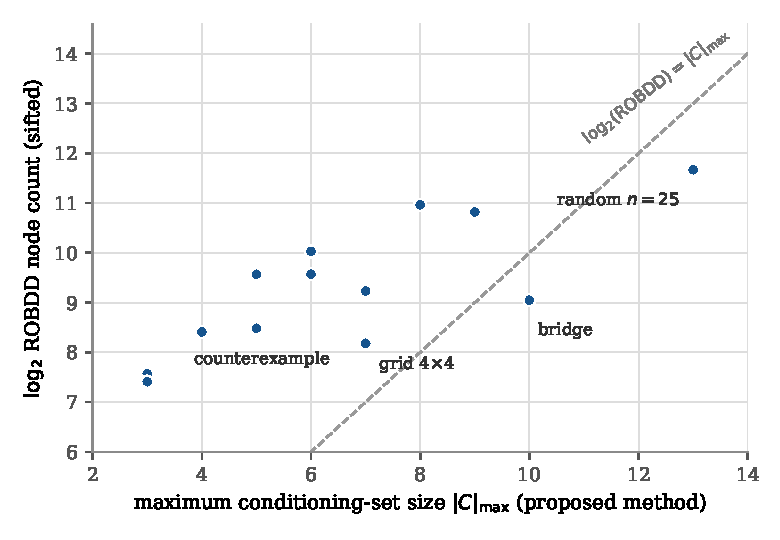
\includegraphics[width=0.75\linewidth]{images/width_correlation.pdf}
\caption{\DIFaddFL{IPA's maximum conditioning-set size against the logarithm of the sifted ROBDD node count, across the complexity-validation networks. Both quantities measure the same structural width; neither method dominates.}}
\label{fig:width}
\end{figure}
\DIFaddend 

\DIFdelbegin \DIFdel{Six Pareto-optimal configurations are analysed. These span a wide range of graph sizes and reconvergent dependency structures. Table~\ref{tab:pareto_structure} summarises the basic structural characteristics of }\DIFdelend \DIFaddbegin \subsection{\DIFadd{Imprecise Reliability Propagation}}\label{sec:imprecise}

\DIFadd{The results so far establish that IPA matches a well-ordered decision diagram on exact point-valued reliability, at a comparable realised amount of work. This section presents the capability that separates the two: the propagation scheme accepts interval- and p-box-valued component reliabilities directly (Section~\ref{subsec:impreciseinputs}).
}

\subsubsection{\DIFadd{Interval-valued reliabilities: exact and fast}}\label{sec:interval}

\DIFadd{Because $b(v)$ is non-decreasing in every component reliability (Section~\ref{sec:model}), its exact range over interval inputs is attained at the two extreme corners of the input box: the lower bound when every component takes its lower reliability, the upper bound when every component takes its upper reliability. This was verified across the full corpus of Section~\ref{sec:comparison} by comparing the propagated interval against the decision-diagram evaluation at both corner inputs: the worst discrepancy in either bound is of order $10^{-16}$. Interval propagation that ignores reconvergent dependence, by contrast, over-widens the range by up to $0.45$ across the corpus, showing that }\DIFaddend the \DIFdelbegin \DIFdel{resulting DAGs. }\DIFdelend \DIFaddbegin \DIFadd{conditioning machinery of Section~\ref{sec:decomp} is as necessary for sound imprecise propagation as it is for exact point values.
}\DIFaddend 

\DIFaddbegin \DIFadd{The interval computation is also fast. For a one-shot query (given a network, produce the interval reliability), IPA completed faster than the decision-diagram route to the same answer (build the diagram once, evaluate at both corner inputs) on every one of eight corpus families tested, by factors ranging from $3.9$ to $99.9$ (Table~\ref{tab:interval_timing}). The diagram route's time is nearly flat, between $44$ and $57$\,ms, across the six smallest networks of the table, and the same holds across the corpus of Table~\ref{tab:corpus}: the sifted build takes a median of $38$ to $45$\,ms for the $84$ graphs whose diagrams have fewer than $1{,}000$ nodes, and grows only beyond that. These ratios therefore partly reflect a per-build cost that does not depend on network size at this scale, and they are smaller on the larger networks. This claim is scoped to the one-shot cost, in which the diagram's construction cost counts against it; a workload that amortises a single construction across many repeated queries on a fixed network is a different scenario, not tested here, and could favour the diagram route instead.
}

\DIFaddend \begin{table}[ht]
\DIFdelbeginFL %DIFDELCMD < \caption{%
{%DIFAUXCMD
\DIFdelFL{Structural characteristics of Pareto-optimal drone network DAGs}}
%DIFAUXCMD
%DIFDELCMD < \label{tab:pareto_structure}
%DIFDELCMD < %%%
\DIFdelendFL \centering\DIFdelbeginFL %DIFDELCMD < \adjustbox{max width=\textwidth}{
%DIFDELCMD < \begin{tabular}{lrrrrrr}
%DIFDELCMD < \toprule
%DIFDELCMD < \textbf{Network} & \textbf{Nodes} & \textbf{Edges} & \textbf{Sources} & \textbf{Sinks} & \textbf{Joins} & \textbf{DiamJoins} \\
%DIFDELCMD < \midrule
%DIFDELCMD < PP1-HighRes-FW    & 145 & 327 & 23 &  99 & 50 & 24 \\
%DIFDELCMD < PP2-HighRes-VTOL  & 171 & 280 & 12 & 131 & 70 & 52 \\
%DIFDELCMD < PP3-MedRes-Sparse &  98 & 223 & 23 &  58 & 25 & 19 \\
%DIFDELCMD < PP4-LowRes-Min    &  39 &  28 &  8 &  24 &  0 &  0 \\
%DIFDELCMD < PP5-MedRes-FW     &  89 & 214 & 23 &  49 & 25 & 21 \\
%DIFDELCMD < PP6-Balanced      &  98 & 261 &  6 &  59 & 34 & 32 \\
%DIFDELCMD < \bottomrule
%DIFDELCMD < \end{tabular}}
%DIFDELCMD < \begin{minipage}{\textwidth}
%DIFDELCMD < \footnotesize
%DIFDELCMD < %%%
\DIFdelFL{Joins = nodes with multiple parents. DiamJoins = join nodes that are diamond join points (reconvergent paths from shared ancestors). }%DIFDELCMD < \end{minipage}
%DIFDELCMD < %%%
\DIFdelendFL \DIFaddbeginFL \small
\caption{\DIFaddFL{One-shot interval reliability: IPA against the decision-diagram route (build once, evaluate at both corner inputs), warm-measured. IPA is faster on every family tested; the comparison is scoped to one-shot queries.}}
\label{tab:interval_timing}
\begin{tabular}{lrrrrrr}
\toprule
\DIFaddFL{Network }& \DIFaddFL{$|V|$ }& \DIFaddFL{$|E|$ }& \DIFaddFL{ROBDD }& \DIFaddFL{IPA (ms) }& \DIFaddFL{ROBDD route (ms) }& \DIFaddFL{ratio }\\
\midrule
\DIFaddFL{counterexample       }& \DIFaddFL{15 }& \DIFaddFL{23 }&  \DIFaddFL{323 }&  \DIFaddFL{0.819 }&  \DIFaddFL{44.603 }& \DIFaddFL{54.5 }\\
\DIFaddFL{multi-source         }& \DIFaddFL{25 }& \DIFaddFL{57 }& \DIFaddFL{5622 }& \DIFaddFL{22.422 }& \DIFaddFL{175.497 }&  \DIFaddFL{7.8 }\\
\DIFaddFL{grid $4\times4$      }& \DIFaddFL{16 }& \DIFaddFL{21 }&  \DIFaddFL{248 }&  \DIFaddFL{0.517 }&  \DIFaddFL{51.654 }& \DIFaddFL{99.9 }\\
\DIFaddFL{layered $4\times6$   }& \DIFaddFL{23 }& \DIFaddFL{35 }&  \DIFaddFL{484 }&  \DIFaddFL{4.619 }&  \DIFaddFL{52.075 }& \DIFaddFL{11.3 }\\
\DIFaddFL{bridge               }& \DIFaddFL{16 }& \DIFaddFL{25 }&  \DIFaddFL{529 }& \DIFaddFL{11.571 }&  \DIFaddFL{48.515 }&  \DIFaddFL{4.2 }\\
\DIFaddFL{series--parallel     }& \DIFaddFL{23 }& \DIFaddFL{32 }&  \DIFaddFL{215 }&  \DIFaddFL{2.429 }&  \DIFaddFL{57.304 }& \DIFaddFL{23.6 }\\
\DIFaddFL{complete-8           }&  \DIFaddFL{8 }& \DIFaddFL{28 }&  \DIFaddFL{685 }&  \DIFaddFL{1.537 }&  \DIFaddFL{49.466 }& \DIFaddFL{32.2 }\\
\DIFaddFL{random $n{=}25$      }& \DIFaddFL{25 }& \DIFaddFL{53 }& \DIFaddFL{4146 }& \DIFaddFL{27.844 }& \DIFaddFL{107.875 }&  \DIFaddFL{3.9 }\\
\bottomrule
\end{tabular}
\DIFaddendFL \end{table}

\DIFdelbegin \DIFdel{To characterise the reconvergent complexity more directly, Table~\ref{tab:diamond_complexity} reports the number of identified diamonds, the number of diamond join nodes, the ratio of diamonds to diamond joins (D/DJ), }\DIFdelend \DIFaddbegin \subsubsection{\DIFadd{Probability-box reliabilities: guaranteed distributional bounds}}\label{sec:pbox}

\DIFadd{At a join resolved by conditioning with p-box inputs, the belief is a convex combination $W\cdot A+(1-W)\cdot B$, where $W$ is the uncertain probability of the conditioning state and $A,B$ are the uncertain conditional beliefs of the two branches. $A$ }\DIFaddend and \DIFaddbegin \DIFadd{$B$ are functions of shared upstream reliabilities and are therefore dependent; treating the combination as an independent sum is unsound and can assign probability mass outside $[0,1]$. IPA instead integrates over the distribution of $W$, combining the branch distributions at each weight level, with the branch dependence bounded by the Fr\'echet--Hoeffding inequalities~\mbox{%DIFAUXCMD
\cite{williamson_probabilistic_1990}}\hskip0pt%DIFAUXCMD
. Soundness of the resulting bounds is inherited from that classical result: the computed pair of distribution functions encloses the true distribution of }\DIFaddend the \DIFdelbegin \DIFdel{maximum observed nesting depth}\DIFdelend \DIFaddbegin \DIFadd{node reliability under any dependence between the branches. A tighter variant restricts the dependence bound to non-negative dependence, motivated by both branches being non-decreasing functions of the shared upstream reliabilities and so unable to be negatively dependent; this variant produced no soundness violation in any validation configuration tested (dozens of topology, input-shape, and uncertainty-width combinations, each checked against Monte Carlo ground truth), but a general proof of its soundness under partial dependence information of this kind is not available and is future work. Every headline claim in this paper uses only the provable Fr\'echet-based bound}\DIFaddend .

\DIFdelbegin \DIFdel{The main computation cost of the algorithmic flow comes form the complexity of diamond decomposition and super-node creation and reuse rate.  
Table~\ref{tab:diamond_complexity} compares the diamond structure characteristics between all six networks. 
}\DIFdelend \DIFaddbegin \DIFadd{Bound tightness, as distinct from soundness, depends on the network's structure. Across a sweep of input-distribution shapes, uncertainty widths, and reconvergence regimes on the benchmark grid network of Section~\ref{sec:grid}, the certified band ranged from approximately $0.18$ of the unit range under high-reliability, weakly reconvergent conditions to approximately $0.70$ under strongly reconvergent, fully uncertain conditions, with zero soundness violations across the sweep (Figure~\ref{fig:envelope}). Reconvergence depth combined with input uncertainty drives tightness; the shape of the input distribution is secondary.
}\DIFaddend 

\DIFdelbegin %DIFDELCMD < \begin{table}[ht]
%DIFDELCMD < %%%
%DIFDELCMD < \caption{%
{%DIFAUXCMD
\DIFdelFL{Diamond-structure complexity metrics for the derived drone network DAGs.}}
%DIFAUXCMD
%DIFDELCMD < \label{tab:diamond_complexity}
%DIFDELCMD < %%%
\DIFdelendFL \DIFaddbeginFL \begin{figure}[ht]
\DIFaddendFL \centering
\DIFdelbeginFL %DIFDELCMD < \adjustbox{max width=\textwidth}{
%DIFDELCMD < \begin{tabular}{lrrrr}
%DIFDELCMD < \toprule
%DIFDELCMD < \textbf{Network} & \textbf{Diamonds} & \textbf{DiamJoins} & \textbf{D/DJ} & \textbf{MaxDepth} \\
%DIFDELCMD < \midrule
%DIFDELCMD < PP4-LowRes-Min    &   0 &  0 &  ---  &  0 \\
%DIFDELCMD < PP2-HighRes-VTOL  & 219 & 52 &  4.2  &  9 \\
%DIFDELCMD < PP6-Balanced      & 203 & 32 &  6.3  & 12 \\
%DIFDELCMD < PP3-MedRes-Sparse & 165 & 19 &  8.7  & 16 \\
%DIFDELCMD < PP5-MedRes-FW     & 177 & 21 &  8.4  & 16 \\
%DIFDELCMD < PP1-HighRes-FW    & 277 & 24 & 11.5  & 18 \\
%DIFDELCMD < \bottomrule
%DIFDELCMD < \end{tabular}}
%DIFDELCMD < \begin{minipage}{\textwidth}
%DIFDELCMD < \footnotesize
%DIFDELCMD < %%%
\DIFdelFL{D/DJ = diamonds per diamond join, indicating the average concentration of nested diamonds around each reconvergent join node. MaxDepth = maximum observed nesting depth of diamond structures.
}%DIFDELCMD < \end{minipage}
%DIFDELCMD < \end{table}
%DIFDELCMD < %%%
\DIFdelend \DIFaddbegin 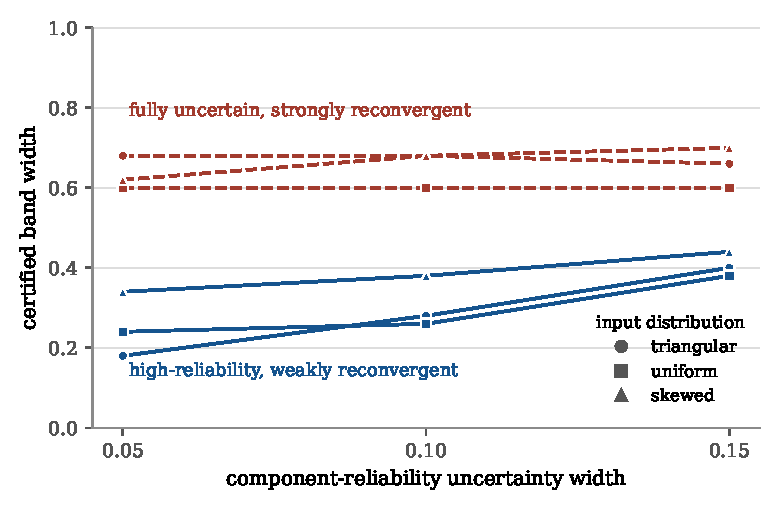
\includegraphics[width=0.8\linewidth]{images/envelope.pdf}
\caption{\DIFadd{Tightness envelope of the certified p-box bound on the benchmark network: band width against component-reliability uncertainty width, for three input-distribution shapes and two reconvergence regimes. Soundness holds in every configuration; only tightness varies, and it is driven by the regime, not the input shape.}}
\label{fig:envelope}
\end{figure}
\DIFaddend 

\DIFdelbegin \DIFdel{The diamonds-per-diamond-join ratio (D/DJ)indicates how many diamonds are concentrated at each diamond join point on average. A higher D/DJ suggests that individual join nodes participate in more nested diamond structures. PP1 has the highest D/DJ (11.5), consistent with its deep nesting structure. PP2 has the lowest D/DJ (4.2) among networks with diamonds, reflecting its wide, shallow topology with many diamond joins but less nesting per join}\DIFdelend \DIFaddbegin \DIFadd{Computational cost is controllable rather than fixed. Interval propagation costs a small constant factor over point-valued propagation (about $1.8$ in our measurements: $0.465$\,ms against $0.819$\,ms on the counterexample-n15 network of Table~\ref{tab:structured}), while p-box propagation grows with the discretisation level of the distribution bounds: $1.54$\,s, $8.68$\,s, $51.02$\,s, and $339.02$\,s at $25$, $50$, $100$, and $200$ levels respectively on that same counterexample network, each measured as a single propagation in its own fresh process (a shared warm process inflates later, larger measurements, so one clean process per measurement is used throughout this paper). The resulting exponent is approximately $2.6$ over this range and increases toward its upper end; propagation beyond $200$ levels is impractical on this network and is not used. Bound tightness is therefore always stated at the discretisation level used. Distributional propagation is not cheap, but its cost is controllable and the bounds are rigorous at every setting.
}

\DIFadd{The same realised-work quantity that governs Float64 and interval cost (Section~\ref{sec:complexity}) also governs p-box cost, at a fixed discretisation level. Figure~\ref{fig:pbox_cost} plots p-box propagation time at steps$=50$ against the realised sub-problem count already reported for the exact and interval comparison, across 14 networks spanning a $141\times$ range in that count. The relationship is close to linear on log-log axes, with time per sub-problem clustered within roughly $0.14$--$0.26$\,s throughout; the raw conditioning-set-width bound $2^{|C|}$, by contrast, does not correlate this cleanly, since two networks with similar bounds can differ substantially in realised sub-problems after memoisation}\DIFaddend .

\DIFdelbegin \DIFdel{The D/DJ ratio correlates with nesting depth across these configurations: higher D/DJ networks tend to have deeper nesting. However, the relationship is nondeterministic: PP3 and PP5 have similar D/DJ ratios (8.7 and 8.4) and identical maximum depth (16) but different computation times (281s vs 256s), showing that other structural factors also affect performance. }\DIFdelend \DIFaddbegin \begin{figure}[ht]
\centering
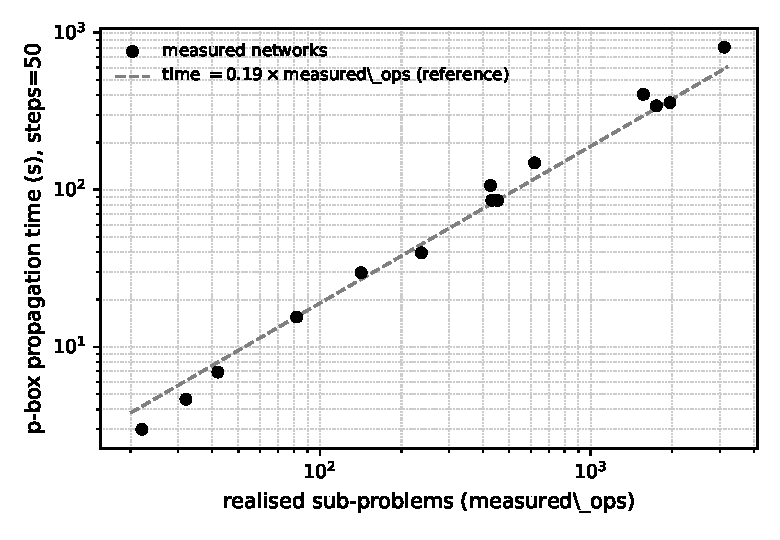
\includegraphics[width=0.75\linewidth]{images/pbox_cost.pdf}
\caption{\DIFaddFL{p-box propagation time at a fixed discretisation level (steps$=50$) against the realised sub-problem count (measured\_ops) already reported for the exact/interval cost comparison (Section~\ref{sec:complexity}), across 14 networks spanning a $141\times$ range. Each point is a single clean measurement, one propagation per fresh process. The near-linear relationship shows that the same realised-work quantity governing Float64/interval cost also governs p-box cost, at a roughly constant price per resolved sub-problem for a given discretisation level.}}
\label{fig:pbox_cost}
\end{figure}
\DIFaddend 

\DIFdelbegin \subsubsection{\DIFdel{Effect of diamond structure on runtime}}
%DIFAUXCMD
\addtocounter{subsubsection}{-1}%DIFAUXCMD
\DIFdelend \DIFaddbegin \subsubsection{\DIFadd{A certified decision bound from a single propagation}}\label{sec:certified}
\DIFaddend 

The \DIFdelbegin \DIFdel{dominant computational cost in IPA arises from the decomposition of reconvergent structures, the construction of supernodes, and the extent to which resolved supernodes can be reused across downstream conditioning contexts.
In the absence of progressive decomposition, the cost of evaluating nested diamonds grows exponentially with the number of conditioning variables and increases further with the size of the nested subgraphs. }\DIFdelend \DIFaddbegin \DIFadd{propagated distribution bounds certify decision-relevant probabilities directly. For a stated reliability requirement $x^\ast$ at a given node, the propagated p-box yields guaranteed lower and upper bounds on $P(b(v)\le x^\ast)$, the probability that the node fails its requirement, from one propagation. On the benchmark network at a representative requirement $x^\ast=0.95$, the certified band on this probability had width between $0.02$ and $0.12$ across the regimes tested (Table~\ref{tab:certified}). Matching that precision by simulation, planned conservatively without foreknowledge of the answer, would require between $267$ and $9{,}604$ samples of the network's uncertain inputs, and the result would remain a statistical estimate, not a guarantee. A decision-diagram method has no analytic route to this bound and would itself fall back on simulation; this certified-bound capability, not raw speed, is the concrete engineering value of imprecise propagation.
}\DIFaddend 

\DIFdelbegin \DIFdel{Three structural factors were observed to strongly influence runtime in the six derived networks: }%DIFDELCMD < \begin{enumerate}
\begin{enumerate}%DIFAUXCMD
%DIFDELCMD <     \item %%%
\item%DIFAUXCMD
\textbf{\DIFdel{Diamond nesting depth.}} %DIFAUXCMD
\DIFdel{Deeply nested diamonds require repeated layers of conditional evaluation and are the strongest driver of computational growth. }%DIFDELCMD < \item %%%
\item%DIFAUXCMD
\textbf{\DIFdel{Conditioning-set size.}} %DIFAUXCMD
\DIFdel{Diamonds with many shared upstream nodes require more conditioning states. }%DIFDELCMD < \item %%%
\item%DIFAUXCMD
\textbf{\DIFdel{Contextual entry points.}} %DIFAUXCMD
\DIFdel{When a resolved diamond receives additional context-dependent inputs from outer conditioning states, reuse of its supernode representation becomes less effective. }
\end{enumerate}%DIFAUXCMD
%DIFDELCMD < \end{enumerate}
%DIFDELCMD < 

%DIFDELCMD < %%%
\DIFdel{Table~\ref{tab:complexity_spectrum} summarises the observed relationship between nesting depth and practical applicability given the structure of the drone network. }%DIFDELCMD < 

%DIFDELCMD < %%%
\DIFdelend \begin{table}[ht]
\DIFdelbeginFL %DIFDELCMD < \caption{%
{%DIFAUXCMD
\DIFdelFL{Empirical tractability spectrum for exact reliability analysis with IPA on the derived drone network DAGs.}}
%DIFAUXCMD
%DIFDELCMD < \label{tab:complexity_spectrum}
%DIFDELCMD < %%%
\DIFdelendFL \centering\DIFdelbeginFL %DIFDELCMD < \adjustbox{max width=\textwidth}{
%DIFDELCMD < \begin{tabular}{lll}
%DIFDELCMD < \toprule
%DIFDELCMD < \textbf{Nesting Depth} & \textbf{Computation Time} & \textbf{Practical Use} \\
%DIFDELCMD < \midrule
%DIFDELCMD < 0 (tree)   & $<$0.1s   & Real-time analysis \\
%DIFDELCMD < 9--12      & $<$1s     & Interactive analysis \\
%DIFDELCMD < 16         & $\sim$5 min & Batch processing \\
%DIFDELCMD < 18+        & Intractable & Beyond practical exact analysis  \\
%DIFDELCMD < \bottomrule
%DIFDELCMD < \end{tabular}}
%DIFDELCMD < %%%
\DIFdelendFL \DIFaddbeginFL \small
\caption{\DIFaddFL{Certified bound on the requirement-violation probability $P(b(v)\le0.95)$ at the benchmark network's target node, from a single propagation, against the Monte Carlo sample count required to match the certified precision under worst-case a-priori planning.}}
\label{tab:certified}
\begin{tabular}{llccc}
\toprule
\DIFaddFL{Regime }& \DIFaddFL{Uncertainty width }& \DIFaddFL{Certified band }& \DIFaddFL{Band width }& \DIFaddFL{MC samples }\\
\midrule
\DIFaddFL{perfect components   }& \DIFaddFL{0.05      }& [\DIFaddFL{0.000, 0.020}] & \DIFaddFL{0.02 }& \DIFaddFL{9}{\DIFaddFL{,}}\DIFaddFL{604 }\\
\DIFaddFL{perfect components   }& \DIFaddFL{0.10      }& [\DIFaddFL{0.000, 0.100}] & \DIFaddFL{0.10 }& \DIFaddFL{385 }\\
\DIFaddFL{perfect components   }& \DIFaddFL{0.15      }& [\DIFaddFL{0.000, 0.120}] & \DIFaddFL{0.12 }& \DIFaddFL{267 }\\
\DIFaddFL{uncertain components }& \DIFaddFL{0.05--0.15 }& [\DIFaddFL{0.980, 1.000}] & \DIFaddFL{0.02 }& \DIFaddFL{9}{\DIFaddFL{,}}\DIFaddFL{604 }\\
\bottomrule
\end{tabular}
\DIFaddendFL \end{table}

\DIFdelbegin \DIFdel{This table should be interpreted as an empirical summary of the present dataset rather than as a universal complexity law. Nevertheless, it provides a useful practical guideline: in these networks, }\DIFdelend \DIFaddbegin \subsection{\DIFadd{Applied Case Study: A Medical Drone Logistics Network for Scotland}}\label{sec:drone}

\DIFadd{With the methodology validated in Sections~\ref{sec:grid}--\ref{sec:imprecise}, this section applies IPA to a real infrastructure planning problem: the conceptual medical drone delivery network for Scotland designed by Jones et al.~\mbox{%DIFAUXCMD
\cite{jones_drone_2025}}\hskip0pt%DIFAUXCMD
. Jones et al. optimised station placement and network structure over real hospital, airport, and candidate-station locations, using stated infrastructure specifications and two drone types: a short-range vertical take-off and landing craft (nominal range 70\,km) and a long-range fixed-wing craft (nominal range 700\,km). Their optimisation trades off delivery time, capital cost, and resilience, and their framework uses point probabilities. The question addressed here is how confidently each location in a candidate design can be said to be reachable from the supply hubs, given the uncertainty in the component availability assumptions.
}

\subsubsection{\DIFadd{Building the reliability model from the source study}}\label{sec:provenance}

\DIFadd{The source study's resilience analysis treats non-hub locations as failing independently with probability $0.2$ and hub locations as always available. The reliability model keeps this structure but represents non-hub availability as the interval $[0.75,0.85]$, centred on the source study's own $0.8$ success probability. The $0.2$ figure is an assumption in the source study, not a value derived from data, so the interval turns the analysis into a sensitivity check on that single assumption. Hub locations keep availability $1$.
}

\DIFadd{Connections follow the source study's construction rule: a connection between two locations exists, for a given drone type, exactly when the distance between them is within that type's nominal range. Where both drone types can serve a connection, the link is available if either succeeds, and }\DIFaddend the \DIFdelbegin \DIFdel{transition from interactive to impractical runtime is relatively sharp once nesting depth exceeds approximately 12--16 levels}\DIFdelend \DIFaddbegin \DIFadd{two transmissions are independent. The model adds one element to connection reliability. The source study holds weather constant while noting that weather-driven range variation is an uncertain quantity that would need expert elicitation. A connection well within a drone's nominal range is treated as reliable, as in the source study. A connection within the final ten per cent of the nominal range, an illustrative weather-derating margin, is given the vacuous transmission probability $[0,1]$, which expresses that adverse weather may or may not close the route. All other probabilities come from the source study.
}

\DIFadd{The dependency graph is directed from the hub tier outward. The source study's connections are undirected, since a route can be flown either way, but the reliability question is whether supply reaches each facility from the hubs. The directed graph follows the study's hub-and-spoke architecture, and source-to-node reachability is computed on the resulting acyclic structure}\DIFaddend .

\DIFdelbegin \subsubsection{\DIFdel{Pareto Network Results}}
%DIFAUXCMD
\addtocounter{subsubsection}{-1}%DIFAUXCMD
\DIFdelend \DIFaddbegin \DIFadd{The source study's optimised network layouts are not published, so three configurations are built as proxies for the qualitative character of three trade-off points it describes. They are not reproductions of an optimisation output. The first is a fixed-wing-reliant centralised design that serves remote locations through a hub backbone (217 locations, 263 connections). The second is a densely interconnected short-range design (242 locations, 1}{\DIFadd{,}}\DIFadd{753 connections). The third is a minimal-investment design that keeps only pre-existing, non-optional infrastructure (230 locations, 1}{\DIFadd{,}}\DIFadd{648 connections). The centralised design is sparse (mean in- and out-degree $1.2$, maximum out-degree $27$ at a hub) and close to tree-like; the other two are far denser (mean degree $7.2$, maximum out-degree $104$ at a hub), with individual facilities served by as many as $16$--$17$ alternate incoming routes, the same per-facility redundancy that produces the conditioning widths reported below.
}\DIFaddend 

\DIFdelbegin \DIFdel{Table~\ref{tab:pareto_timing} compares IPA runtime for each network configuration, ordered by computation time. }\DIFdelend \DIFaddbegin \subsubsection{\DIFadd{Redundancy and the practical boundary of exact analysis}}\label{sec:redundancy}
\DIFaddend 

\DIFdelbegin %DIFDELCMD < \begin{table}[ht]
%DIFDELCMD < %%%
%DIFDELCMD < \caption{%
{%DIFAUXCMD
\DIFdelFL{IPA runtime across Pareto-optimal drone network configurations.}}
%DIFAUXCMD
%DIFDELCMD < \label{tab:pareto_timing}
%DIFDELCMD < \centering
%DIFDELCMD < \adjustbox{max width=\textwidth}{
%DIFDELCMD < \begin{tabular}{lrrrl}
%DIFDELCMD < \toprule
%DIFDELCMD < \textbf{Network} & \textbf{MaxDepth} & \textbf{D/DJ} & \textbf{Time} & \textbf{Category} \\
%DIFDELCMD < \midrule
%DIFDELCMD < PP4-LowRes-Min    &  0 & --- &    0.02s & Tree structure \\
%DIFDELCMD < PP6-Balanced      & 12 & 6.3 &    0.02s & Shallow nesting \\
%DIFDELCMD < PP2-HighRes-VTOL  &  9 & 4.2 &    0.31s & Shallow nesting \\
%DIFDELCMD < PP5-MedRes-FW     & 16 & 8.4 &     256s & Deep nesting \\
%DIFDELCMD < PP3-MedRes-Sparse & 16 & 8.7 &     281s & Deep nesting \\
%DIFDELCMD < PP1-HighRes-FW    & 18 & 11.5 &  $>$600s & Beyond practical range  \\
%DIFDELCMD < \bottomrule
%DIFDELCMD < \end{tabular}}
%DIFDELCMD < \end{table}
%DIFDELCMD < 

%DIFDELCMD < %%%
\DIFdel{The results show that runtime is governed primarily by reconvergent nesting depth rather than by graph size alone. For example, PP2 has 171 nodes and 219 diamonds but completes in 0.31 seconds as a result of its  shallower nesting (depth 9). Comparing this to PP3 which  has fewer nodes (98) and fewer diamonds (165)but still requires 281 seconds because of deep nesting (depth }\DIFdelend \DIFaddbegin \DIFadd{The reconvergent structure of each configuration is controlled by a network-design parameter: the number of alternate routes provisioned per location. This is a redundancy choice in the network design, not a parameter of the analysis method. Connecting every operationally plausible pair of locations makes exact diamond identification itself impractical. Identification demanded more than 25\,GB on a }\DIFaddend 16\DIFdelbegin \DIFdel{). On the extreme case, PP1 with nesting depth 18  falls beyond the practical range for interactive exact analysis . 
Comparing compuataional costs, it is clear that the transition between tractable and intractable  occurs sharply. Networks with nesting depth $\leq$12 complete in under one second regardless of diamond count. The two larger networks with depth }\DIFdelend \DIFaddbegin \DIFadd{\,GB workstation within about fifteen minutes and did not complete. Limiting the provision to sixteen alternate routes per location brings the conditioning requirement to }\DIFaddend 16 \DIFdelbegin \DIFdel{take a lot more time and by depth 18, the run time starts to exceed practical limits. These results support the central claim of the paper: the principal determinant of tractability in exact DAG reliability analysis is notthe raw number of nodes or edges, but the arrangement and nesting depth of dependency-inducing reconvergent structures}\DIFdelend \DIFaddbegin \DIFadd{in both dense configurations. Further increases in provisioned routes changed neither the requirement nor the runtime materially, which indicates that the reconvergent structure of this network saturates at that level. Full exact interval propagation on the densest configurations completes in under 25 seconds, and on the centralised configuration, whose conditioning requirement is 8, in well under one second}\DIFaddend . \DIFaddbegin \DIFadd{The practical boundary of exact analysis on this network is therefore a measured quantity expressed through a design parameter: more provisioned redundancy improves resilience and raises the cost of verifying it exactly.
}\DIFaddend 

\DIFaddbegin \DIFadd{The comparison of Section~\ref{sec:comparison} was repeated on these networks. On the centralised configuration the two methods agree to floating-point precision, and IPA's one-shot interval computation takes $0.008$\,s against $0.463$\,s for the decision-diagram route to the same interval, about $56$ times faster (diagram size 2}{\DIFadd{,}}\DIFadd{667 nodes). On the minimal-investment topology with six alternate routes per location, the agreement is $1.1\times10^{-16}$ and IPA takes $0.104$\,s against $1.579$\,s, about $15$ times faster (diagram size 4}{\DIFadd{,}}\DIFadd{968 nodes). With sixteen alternate routes per location on the same topology, the decision-diagram build did not complete within a practical computational budget under either of two variable-ordering strategies, while IPA completed the full exact computation in under 25 seconds. Both methods are governed by the same structural width and both are practical at low redundancy. On this network, measured along a real redundancy design parameter, IPA remains practical at a redundancy level where the decision-diagram build does not; the crossover between the two has not been located precisely, and the result is specific to this network and not a general statement about decision-diagram methods.
}

\DIFaddend \subsubsection{\DIFdelbegin \DIFdel{Summary of the case-study }\DIFdelend \DIFaddbegin \DIFadd{Reliability }\DIFaddend findings}\DIFaddbegin \label{sec:findings}
\DIFaddend 

\DIFdelbegin \DIFdel{The two case studies support three main conclusions. First, IPA reproduces exact node reliabilities on a benchmark reconvergent DAG and compares favourably with the published dPrPm results. Second, IPA remains computationally efficient on realistic infrastructure DAGs when reconvergent structures are shallow or moderately nested. Third, the practical limit of exact analysis is controlled primarily by the depth and reuse characteristics of nested diamond structures rather than by overall network size alone. }%DIFDELCMD < 

%DIFDELCMD < %%%
\DIFdel{These observations motivate the use of IPA as an exact reliability analysis tool for a broad class of acyclic process systems, while also clarifying the structural regimes in which approximation methods may still be required}\DIFdelend \DIFaddbegin \DIFadd{Table~\ref{tab:drone} summarises the propagated interval reliabilities. In the centralised configuration the propagated bounds are narrow (mean band width $0.089$, maximum $0.100$). Each location's reachability essentially inherits the availability band assumed for the locations themselves, so the network adds little uncertainty, but it also adds little protection: the design is tree-like, and a single-route failure disconnects service. In the two higher-redundancy configurations the best-connected locations are reachable with near-certainty, while the worst-served locations show a decision-relevant spread. The least certain facility, Islay Hospital, an island site, has reachability probability bounded between $0.56$ and $0.72$. A point-probability analysis cannot distinguish a facility whose reachability is confidently $0.6$ from one whose reachability lies anywhere between $0.56$ and $0.72$, yet the two call for different interventions. Figure~\ref{fig:map} colours the network by the lower reliability bound and by band width. It identifies the facilities where additional redundancy, or better component-availability data, would most improve either the network or our knowledge of it, and these are concentrated in the islands and the far north}\DIFaddend .

\DIFaddbegin \begin{table}[ht]
\centering\small
\caption{\DIFaddFL{The three proxy configurations: structure, conditioning requirement, and the propagated reliability bounds. Every belief is contained in $[0,1]$ with lower $\le$ upper (soundness); the worst-served facility in both dense configurations is Islay Hospital.}}
\label{tab:drone}
\begin{tabular}{lrrrccc}
\toprule
\DIFaddFL{Configuration }& \DIFaddFL{$|V|$ }& \DIFaddFL{$|E|$ }& \DIFaddFL{$|C|_{\max}$ }& \DIFaddFL{mean band }& \DIFaddFL{max band }& \DIFaddFL{worst facility }\\
\midrule
\DIFaddFL{fixed-wing centralised }& \DIFaddFL{217 }& \DIFaddFL{263 }& \DIFaddFL{8 }& \DIFaddFL{0.089 }& \DIFaddFL{0.100 }& [\DIFaddFL{0.750, 0.850}] \\
\DIFaddFL{dense decentralised    }& \DIFaddFL{242 }& \DIFaddFL{1753 }& \DIFaddFL{16 }& \DIFaddFL{0.094 }& \DIFaddFL{0.160 }& [\DIFaddFL{0.562, 0.722}] \\
\DIFaddFL{concentrated minimal   }& \DIFaddFL{230 }& \DIFaddFL{1648 }& \DIFaddFL{16 }& \DIFaddFL{0.093 }& \DIFaddFL{0.160 }& [\DIFaddFL{0.562, 0.722}] \\
\bottomrule
\end{tabular}
\end{table}

\begin{figure}[ht]
\centering
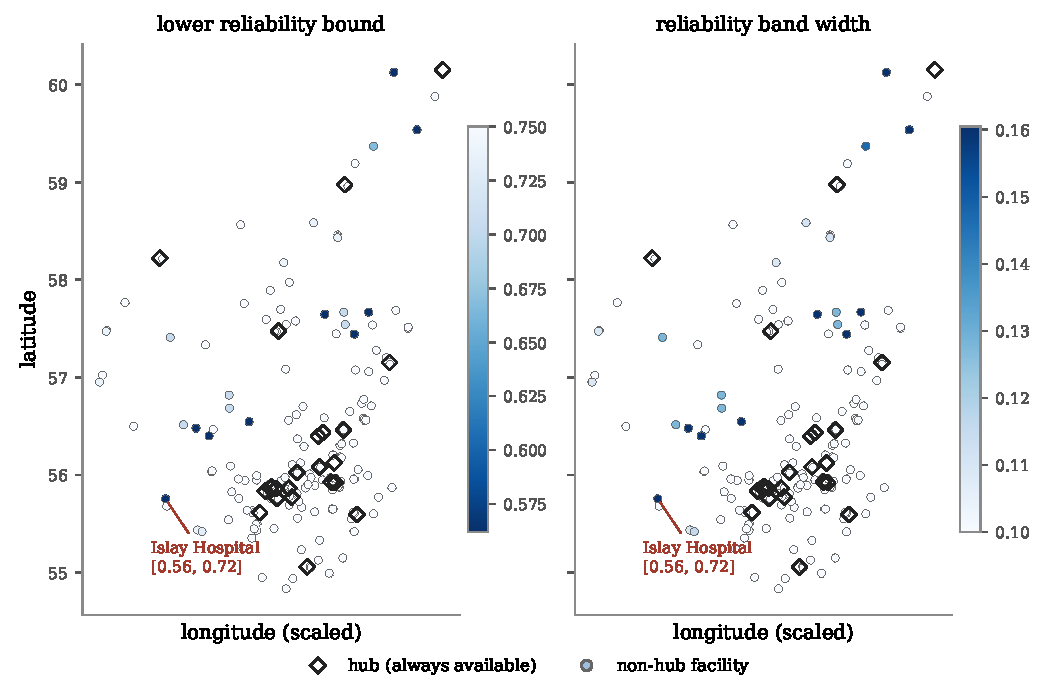
\includegraphics[width=\linewidth]{images/drone_reliability_map.pdf}
\caption{\DIFaddFL{Reliability map of the dense decentralised configuration: each facility coloured by the lower bound of its propagated reachability reliability (left; darker = less certainly reachable) and by the width of its reliability band (right; darker = more uncertainty). Hubs (diamonds) are assumed always available. Uncertainty concentrates at island and far-northern facilities; the worst-served facility, Islay Hospital, is bounded at $[0.56,0.72]$.}}
\label{fig:map}
\end{figure}

\DIFaddend \subsection{\DIFdelbegin \DIFdel{Limitations and Future Work}%DIFDELCMD < \MBLOCKRIGHTBRACE
%DIFDELCMD < %%%
\DIFdel{IPAprovides exact source-to-node reliability values for }\DIFdelend \DIFaddbegin \DIFadd{Adversarial Structure}}\label{sec:adversarial}

\DIFadd{Section~\ref{sec:complexity} used two constructed families, fan-in and mesh, to show where IPA's factorisation helps and where it cannot. This section asks the same question of a real, independently published family, not a hand-built one: the ISCAS85 combinational circuit benchmarks~\mbox{%DIFAUXCMD
\cite{brglez_iscas85_1985}}\hskip0pt%DIFAUXCMD
, a suite of digital logic circuits represented natively as }\DIFaddend directed acyclic graphs\DIFdelbegin \DIFdel{by resolving reconvergent dependencies through conditional decomposition.
Its main limitation is therefore not approximation error, but computational tractability in the presence of deeply nested dependency structures. }\DIFdelend \DIFaddbegin \DIFadd{. Every circuit is assigned the same illustrative, non-degenerate component reliability ($0.9$, uniformly) used throughout this corpus, which is itself a deliberate worst case here: identification excludes a node from a conditioning set only when its reliability is fixed at exactly $0$ or $1$ (Section~\ref{sec:decomp}), so a non-degenerate value everywhere leaves no reconvergent structure excluded from conditioning.
}\DIFaddend 

\DIFdelbegin \DIFdel{For tree-structured networks and for DAGs with shallow or moderately nested diamonds, the algorithm remains efficient because most node updates are local and independent, and only a limited number of reconvergent subgraphs require conditional evaluation.
However, when reconvergent structures become deeply nested, the number of conditioning states grows exponentially. In such cases, progressive decomposition reduces repeated evaluation but cannot eliminate the intrinsic complexity of exact inference. }\DIFdelend \DIFaddbegin \DIFadd{The smallest circuit, }\emph{\DIFadd{c17}} \DIFadd{(11 nodes), is trivial (conditioning width 1) and was fully validated across all three input types, including a p-box propagation whose cost matched the prediction of Section~\ref{sec:pbox}'s realised-work relationship (predicted $1.3$--$2.3$\,s at 50 discretisation levels; measured $1.41$\,s). The next three circuits tested, }\emph{\DIFadd{c432}} \DIFadd{(196 nodes), }\emph{\DIFadd{c499}} \DIFadd{(243 nodes), and }\emph{\DIFadd{c880}} \DIFadd{(443 nodes), reach conditioning widths of 67, 41, and 50 respectively, an order of magnitude beyond any other network in this corpus, placing exact propagation on these circuits well outside a practical budget; two further circuits, }\emph{\DIFadd{c1355}} \DIFadd{and }\emph{\DIFadd{c1908}} \DIFadd{(587 and 913 nodes), exceed the memory available on a 16\,GB workstation during identification itself.
}\DIFaddend 

\DIFdelbegin \DIFdel{The case studies show that three factors are particularly important:
}%DIFDELCMD < \begin{enumerate}
%DIFDELCMD <     \item %%%
\textbf{\DIFdel{Nesting depth.}} %DIFAUXCMD
\DIFdel{Deeply nested diamonds generate repeated conditional branching and are the dominant driver of computational cost.
    }%DIFDELCMD < \item %%%
\textbf{\DIFdel{Conditioning-set size.}} %DIFAUXCMD
\DIFdel{Diamonds with many shared upstream variables require a larger number of conditional states to be evaluated. }%DIFDELCMD < \item %%%
\textbf{\DIFdel{Context-sensitive reuse.}} %DIFAUXCMD
\DIFdel{When the effective input state of a resolved diamond varies across outer conditioning contexts, }\DIFdelend \DIFaddbegin \DIFadd{This is not a boundary specific to IPA. El Fattah and Dechter~\mbox{%DIFAUXCMD
\cite{elfattah_diagnosing_1996}}\hskip0pt%DIFAUXCMD
, studying the same circuits with classical tree-clustering and cutset conditioning, the general method IPA specialises (Section~\ref{sec:complexity}), independently report clique and cutset sizes for c432 that they describe as ``clearly not feasible'' for any exact structural method, and comparably extreme figures for the larger circuits in the suite. Decision-diagram size is governed by the same structural width, so a well-ordered decision diagram meets the same wall on these circuits; it does not resolve it.
}

\subsection{\DIFadd{Limitations and Future Work}}\label{sec:limitations}

\paragraph{\DIFadd{Exact point-valued reliability}} \DIFadd{For point-valued reliability, IPA has no asymptotic advantage over a well-ordered decision diagram: both are exponential in the network's structural width (the conditioning width here, the pathwidth for the diagram), reflecting the \#P-hardness of network reliability, and across the corpus of Section~\ref{sec:comparison} neither dominates. Its distinctive value instead lies in imprecise propagation. Interval results are exact at machine precision, and }\DIFaddend the \DIFdelbegin \DIFdel{reuse of stored supernode maps becomes less effective. }%DIFDELCMD < \end{enumerate}
%DIFDELCMD < 

%DIFDELCMD < %%%
\DIFdel{The current decomposition framework naturally identifies the specific subgraphs responsible for computational intractability.
Rather than approximating the entire network, future work could apply approximation selectively to deeply nested diamonds while maintaining exact computation elsewhere. This would localise approximation error to the structurally difficult parts of the graph and preserve exactness on the remaining network }\DIFdelend \DIFaddbegin \DIFadd{speed comparison of Section~\ref{sec:interval} is scoped to one-shot queries. Distributional bounds are sound, but their tightness is structure-dependent, tight for high-reliability or weakly reconvergent systems and conservative for strongly reconvergent systems with broadly uncertain components, and their cost grows with the discretisation level, which confines full distributional propagation to modest networks at present; for larger networks, interval propagation combined with sampling is the practical recourse. The tighter positive-dependence operator is validated empirically but not proven sound in general; every guaranteed claim in this paper uses the proven Fr\'echet operator instead.
}

\paragraph{\DIFadd{Practical range}} \DIFadd{IPA is exponential in width and intended for the sparse-to-moderate regime, a ceiling shared with every exact method: Section~\ref{sec:adversarial} located it on a real published circuit family, and the applied case study locates it on a real infrastructure network, where a conditioning requirement of 16, reached at sixteen provisioned alternate routes per location, remains practical (tens of seconds), while unrestricted connectivity makes exact diamond identification itself exceed a 16\,GB memory budget before propagation can begin. Imprecise propagation does not relax this boundary: interval and p-box propagation use the same conditioning depth as exact point propagation, and only a change to the network design itself alters the cost. For networks beyond the practical range, a depth-limited hybrid suggests itself: condition exactly to a chosen depth and, beyond it, combine reconvergent contributions without conditioning, which for interval inputs gives a rigorous outer bound (wider, but sound) and for p-box inputs would use the Fr\'echet combination for the unconditioned remainder. This hybrid is proposed, not implemented or evaluated here; the method reported in this paper does not degrade exactness anywhere.
}

\paragraph{\DIFadd{Structural scope}} \DIFadd{The method addresses directed acyclic dependency structures. The applied case study's networks are directed by the hub-and-spoke supply logic of their source design; general cyclic or bidirectional dependency networks, feedback loops and return flows, are outside the present scope, and their principled treatment, for example by unrolling or by strongly-connected-component condensation, is future work}\DIFaddend .
\DIFdelbegin \DIFdel{In the present implementation, diamonds are resolved progressively during evaluation. A useful extension would be to perform a more global preprocessing step to identify the full reconvergent structure of the graph in advance and optimise the order in which diamonds are decomposed. This may reduce repeated work and improve tractability in dense dependency networks.
}\DIFdelend 

\section{Conclusions}\DIFdelbegin \DIFdel{An }\DIFdelend \DIFaddbegin \label{sec:conclusions}

\DIFadd{This paper has presented the Information Propagation Algorithm (IPA), an }\DIFaddend exact reliability analysis method for directed acyclic process networks with reconvergent dependency structures\DIFdelbegin \DIFdel{named Information Propagation Algorithm (IPA) has been proposed}\DIFdelend . The method computes source-to-node reliability by propagating \DIFdelbegin \DIFdel{local }\DIFdelend reachability probabilities in topological order\DIFdelbegin \DIFdel{and }\DIFdelend \DIFaddbegin \DIFadd{, }\DIFaddend resolves dependent incoming signals \DIFdelbegin \DIFdel{through conditional decomposition of }\DIFdelend \DIFaddbegin \DIFadd{by conditioning on separating sets of shared ancestors, and replaces resolved }\DIFaddend fork--join \DIFdelbegin \DIFdel{diamond structures. Once resolved, these structures are replaced by }\DIFdelend \DIFaddbegin \DIFadd{substructures with }\DIFaddend statistically equivalent supernodes\DIFdelbegin \DIFdel{, allowing the graph to be progressively simplified while preserving exactness. This reduces the complexity from $O(2^{\sum c_i} \times \prod d_i)$ without decomposition to $O(\sum 2^{c_i})$ with decomposition for subsequent belief updates on the same diamond structure}\DIFdelend . \DIFaddbegin \DIFadd{IPA is a specialisation of cutset conditioning to source-to-node reachability: its per-instance cost is bounded by $\sum_d 2^{|C_d|}$ over the diamonds resolved, computable before enumeration begins, and an independent-substructure factorisation reduces fan-in conditioning from exponential to linear where independence permits.
}\DIFaddend 

\DIFdelbegin \DIFdel{The proposed method is therefore not only an exact message-passing formulation for DAG reliability, but a structured way of resolving reconvergent dependencies without resorting to global path enumeration. IPA provides an exact and efficient tool for a broad class of acyclic process systems, while also identifying the structural regimes in which approximation methods will still be necessary. }%DIFDELCMD < 

%DIFDELCMD < %%%
\DIFdel{Two case studies were presented to validate }\DIFdelend \DIFaddbegin \DIFadd{Exactness was verified against an independent exact method, a reduced-ordered binary decision diagram with dynamic variable reordering, across 129 random and mutated networks, six topological families, and several structured and real-world networks, with the worst observed disagreement at floating-point precision. The same comparison shows that }\DIFaddend IPA's \DIFdelbegin \DIFdel{effectiveness and accuracy. The comparison against the dPrPm, another message passing algorithm for signal propagation in DAGs, shows a speed-up in the calculation larger than two order of magnitude  while computed the same result as exact path enumeration.
The second case study applied IPA to six Pareto-optimal }\DIFdelend \DIFaddbegin \DIFadd{cost is governed by the same structural width parameter as the diagram's size, and neither method dominates: for exact point-valued reliability IPA is competitive with, not superior to, a well-ordered decision diagram. Its distinguishing capability is the native propagation of imprecise component reliabilities. Interval-valued inputs yield the exact reliability range at machine precision, faster for one-shot queries than the decision-diagram route to the same interval on every family tested. Probability-box inputs yield guaranteed distributional bounds through a conditioning operator grounded in the Fr\'echet--Hoeffding inequalities, which certify requirement-violation probabilities from a single propagation, a result no point-valued exact method produces analytically.
}

\DIFadd{An applied case study of a medical }\DIFaddend drone logistics network \DIFdelbegin \DIFdel{configurations spanning a range of diamond complexity with up to 277 diamonds and a nesting depth of 18. The drone-network case study indicates that networks with moderate numbers of nodes and edges may remain highly tractable if reconvergent structures are shallow (depth $\leq$12), whereas significantly smaller networks may already become impractical for exact analysis if reconvergent dependencies are deeply nested (depth $\geq$18).
}%DIFDELCMD < 

%DIFDELCMD < %%%
\DIFdel{Overall, the results suggest that }\DIFdelend \DIFaddbegin \DIFadd{for Scotland, with every input traced to the source design study and one explicitly flagged extension, illustrates the engineering use of the method: propagated reliability bounds identify the facilities whose delivery reachability is most uncertain under the stated input uncertainty, and a sweep of a real redundancy design parameter locates the practical boundary of }\DIFaddend exact \DIFdelbegin \DIFdel{reliability }\DIFdelend analysis \DIFdelbegin \DIFdel{in large DAGs }\DIFdelend \DIFaddbegin \DIFadd{on the network. Within that boundary, IPA completes full exact propagation in under 25 seconds at a redundancy level where the decision-diagram alternative did not complete within a practical budget. Exact reliability analysis of large acyclic networks }\DIFaddend is feasible whenever dependency-inducing substructures remain sufficiently localised\DIFdelbegin \DIFdel{. This makes IPA particularly relevant for infrastructure design, performance assessment, and decision-support problems in systems that can be represented as multi-source acyclic process networks}\DIFdelend \DIFaddbegin \DIFadd{, and this boundary can be measured and expressed in design terms}\DIFaddend .

\DIFdelbegin \DIFdel{Although the IPA is currently formulated for binary node and edge states in directed acyclic graphs the approach can be generalised to handle cases with }\DIFdelend \DIFaddbegin \DIFadd{Future work includes a soundness proof for the tighter positive-dependence conditioning operator, the depth-limited hybrid scheme proposed for networks beyond the exact range, extension to }\DIFaddend multi-state components \DIFdelbegin \DIFdel{, temporally varying reliabilities, }\DIFdelend and explicitly modelled common-cause failures\DIFdelbegin \DIFdel{beyond structural path sharing.
Future research directions may include developing optimization algorithms that pre-decompose the full network before belief propagation as well as further parallelization opportunities beyond topological layer processing, particularly during diamond decomposition when nested diamonds are not interconnected}\DIFdelend \DIFaddbegin \DIFadd{, and a principled treatment of cyclic dependency structures}\DIFaddend .

\bibliographystyle{elsarticle-num}
\bibliography{references}

\section*{Acknowledgements}
This work was supported by the Nuclear Decommissioning Authority (NDA) in conjunction with the \DIFaddbegin \DIFadd{UK }\DIFaddend National Nuclear Laboratory (\DIFaddbegin \DIFadd{UK}\DIFaddend NNL ) through the NDA Bursary Scheme (project number NNL/UA/118).


\section*{Data and Software Availability}

The implementation of the Information Propagation Algorithm (IPA) \DIFdelbegin \DIFdel{, together with the benchmark datasets and scripts }\DIFdelend \DIFaddbegin \DIFadd{is released as the open-source Julia package }\texttt{\DIFadd{InformationPropagationAnalysis.jl}}\DIFadd{, registered in the Julia General package registry and available at }\url{https://github.com/Temi-Tory/InformationPropagationAnalysis.jl}\DIFadd{. The benchmark networks, validation scripts, and result artefacts }\DIFaddend required to reproduce \DIFdelbegin \DIFdel{the case studies, is available at :
}%DIFDELCMD < 

%DIFDELCMD < \url{https://github.com/Temi-Tory/InformationPropagationAnalysis.jl}%%%
\DIFdelend \DIFaddbegin \DIFadd{every table and figure in this manuscript are deposited at }\url{https://doi.org/10.5281/zenodo.22821307} \DIFadd{under an MIT licence, together with a README mapping each artefact to the manuscript table or figure it supports}\DIFaddend .

\end{document}

\endinput
%%
%% End of file `elsarticle-template-num.tex'.
    